\documentclass[a4paper]{article}
\usepackage{graphicx} % Required for inserting images
\graphicspath{{./images/}}


%% Language and font encodings
\usepackage[english]{babel}
\usepackage[utf8x]{inputenc}
\usepackage[T1]{fontenc}
\usepackage{booktabs}
\usepackage{algorithm}
\usepackage{algorithmicx}
\usepackage{amsfonts}
\usepackage{algpseudocode}
\usepackage{color,soul}
\usepackage{multicol}
\usepackage{amsmath}
\usepackage{amssymb}
\usepackage{calc}
\usepackage{wrapfig}
\usepackage{hyperref}
\usepackage{tikz}  %
\usetikzlibrary{tikzmark}
\usetikzlibrary{positioning}
\usepackage{subcaption}
\usepackage{xcolor}
\usepackage{stmaryrd}
\usepackage{listings}
\usepackage{mathtools}
\usepackage{diagbox}



	% Eingekreiste Nummern für Aufzählungen
	\newcommand*\circled[1]{\tikz[baseline=(char.base)]{
            \node[shape=circle,draw,inner sep=1.2pt] (char) {#1};}}


\usepackage{courier} %% Sets font for listing as Courier.
\usepackage{listings, xcolor}
\lstset{
tabsize = 4, %% set tab space width
showstringspaces = false, %% prevent space marking in strings, string is defined as the text that is generally printed directly to the console
numbers = left, %% display line numbers on the left
commentstyle = \color{orange}, %% set comment color
keywordstyle = \color{blue}, %% set keyword color
stringstyle = \color{red}, %% set string color
rulecolor = \color{black}, %% set frame color to avoid being affected by text color
basicstyle = \small \ttfamily , %% set listing font and size
breaklines = true, %% enable line breaking
numberstyle = \tiny,
}

%%damit I.H über = steht
\newcommand\myEqualOne{\mathrel{\overset{\makebox[0pt]{\mbox{\normalfont\tiny\sffamily I.H}}}{=}}}


%% Sets page size and margins
\usepackage[a4paper,top=3cm,bottom=2cm,left=3cm,right=3cm,
            marginparwidth=1.75cm]{geometry}

%%--------------------------begin Document--------------------------------
\title{Algorithmen und Datenstrukturen 2023}
\author{bergery@student.ethz.ch}
\date{Oktober 2023}

\begin{document}
\maketitle
\begin{center}
    
\includegraphics{Pictures/eth_logo_kurz_pos Kopie.png}
\end{center}

\tableofcontents
\newpage

%%Chapter 01
\section{Vorwort}
Ziel dieses Skriptes ist die Vermittlung eines groben Überblicks über die Vorlesung "Algorithmen und Datenstrukturen". Für die Prüfung sollten die in diesem Skript enthaltenen Informationen vorausgesetzt werden. Für Fehler in diesem Skript wird keine Haftung übernommen.

%%Chapter 02
\section{Mathematische Grundlagen}
\subsection{Induktion}
    Die vollständige Induktion ist eine mathematische Beweismethode, nach der eine Aussage für alle natürlichen Zahlen bewiesen wird, die größer oder gleich einem bestimmten Startwert sind. Da es sich um unendlich viele Zahlen handelt, kann eine Herleitung nicht für jede Zahl einzeln erbracht werden. Sie ist ein deduktives Verfahren. \\
    Der Beweis, dass die Aussage $A(n)$ für alle $n \geq n_0 (n_0$ meist 0 oder 1), gilt, wird dabei in zwei Etappen durchgeführt:
    \begin{enumerate}
        \item Im \textit{Induktionsanfang} wird die Gültigkeit der Aussage $A(n_0)$ für eine kleinste Zahl $n_0$ gezeigt.
        \item Im \textit{Induktionsanfang} wird für ein beliebiges $n \geq n_0$ die Gültigkeit der Aussage $A(n+1)$ aus der Gültigkeit von $A(n)$ geschlussfolgert.
    \end{enumerate}
    \textbf{Beispiel:} \\
        Aussage: $A(n):= 1 + 2 + 3 + ...+ n = \frac{n \cdot (n+1)}{2}$ für $n \geq 1$ \\
        \textit{Base Case}: Für $n = 1$ gilt: $1 = \frac{1 \cdot (1+1)}{2} \rightarrow 1 = 1 \ \checkmark$ \\
        \textit{Induction hypothesis}: "We now assume that it is true for $n = k$, i.e., $1 + 2 + 3 + ...+ k = \frac{k \cdot (k+1)}{2} $.
        \textit{Induction step}: $k \rightarrow k+1$ \\
        $1 + 2 + 3 + ...+ k + (k+1) \myEqualOne  \frac{k \cdot (k+1)}{2} + (k+1)$, where $\frac{k \cdot (k+1)}{2} + (k+1) = \frac{k^2 + 3k + 2}{2} = \frac{(k+1) \cdot (k+2)}{2} \ \square.$
        By the principle of mathematical induction, we conclude that $ 1 + 2 + 3 + ...+ n = \frac{n \cdot (n+1)}{2}$ is true for all $n \in \mathbb{N}.$
        \\
        
    \subsection{Wichtige Annäherungen}
    Damit wir schnelle Resultate erhalten können, sind Approximationen ein fundamentaler Bestandteil. Aus diesem Grund folgende Liste:
%% ERGÄNZUNGEN ERSTELLEN GEORG WEEK 3 => WEEK 4
    \begin{itemize}
        \item  $n! \leq n^n, $ for $  n\geq 1 $ 
        \item $\big(\frac{n}{2}\big)^{{n}/{2}} \leq n!, \ for\ n\geq 1 $
        \item $ \sum_{i=0}^{n} \log n  = \ \log\prod_{i=1}^{n}n = \log{n!} \ \approx n\log n \to\mathcal{O}(n \log n)$
        \item $\sum_{i=0}^{n} 1 = (n+1)  \to \mathcal{O}(n)$
        \item $\sum_{i=0}^{n} i = \frac{n(n+1)}{2} = \sum_{j=1}^n\sum_{k=1}^i 1 \to \mathcal{O}(n^2)$
        \item $\sum_{i=0}^{n} i^2 = \frac{n(n+1)(2n+1)}{6} \to \mathcal{O}(n^3)$
        \item $\sum_{i=0}^{n} i^3 = \frac{n^2(n+1)^2}{4}  \to\mathcal{O}(n^4)$
        \item binomial coefficient: $\binom{n}{k}= \frac{n!}{k!(n-k)!}$
        \item $\binom{n}{0}=\binom{n}{n}=1  \quad\quad
              \binom{n+1}{k+1}=\binom{n}{k}+\binom{n}{k+1}  \quad\quad
              \binom{n}{n-k}=\binom{n}{k}$
        \item $\sum_{i=1}^{n}i^k \leq \sum_{i=1}^{n}n^k$
    \end{itemize}
        

    \subsection{Big-O Notation}
    Landau-Symbole (engl. Big-O notation) werden verwendet, um das asymptotische Verhalten von Funktionen und Folgen zu beschreiben.
    In der Informatik werden sie bei der Analyse von Algorithmen verwendet und geben ein Maß für die Anzahl der Elementarschritte oder der Speichereinheiten in Abhängigkeit von der Größe des gegebenen Problems an. \\
    Für Annäherungen wird auch sehr oft die \textbf{Regel von de l'Hôpital} \label{Hôpital} angewendet:\\
        Let $f, g : \mathbb{R}\to\mathbb{R}$ be differentiable functions with $f(x)\to\infty, g(x)\to\infty$ for $x\to\infty$. \\
        If $\lim_{x\to\infty}\frac{f'(x)}{g'(x)}$ exists, then
        $\lim_{x\to\infty}\frac{f(x)}{g(x)}=\lim_{x\to\infty}\frac{f'(x)}{g'(x)}$


    \subsubsection{Definition O-Notation}
    In der Tabelle (\ref{tab:ONotation}) sehen wir jegliche Definition der $\mathcal{O}$-Notation.
    Wir unterscheiden zwischen, $\Omega$ (Omega) [lower-bound], $\Theta$ (Theta) [tight-bound] und  $\mathcal{O}$ [upper-bound]. Damit dies noch mathematisch formuliert ist haben wird folgendes:   \textbf{Wichtiger Hinweis:} Implikationspfeil anschauen: $\mathcal{O}(f) \implies \lim_{x\to\infty}\frac fg = \infty \ \lightning$ \\
    Let $f, g: \mathbb{R} \rightarrow \mathbb{R}^+$ such that the limit of $\frac f g$ exists. Then:
    
    \begin{equation*}
    \lim_{x\to\infty}\frac fg = \infty \Rightarrow g \in \mathcal{O}(f) \text{ and } f \in \Omega(g)
    \end{equation*}
    \begin{equation*}
    \lim_{x \rightarrow \infty} \frac fg = C \in \mathbb{R}^+ \setminus \left\lbrace 0 \right\rbrace \Rightarrow f \in\Theta(g)  \text{ and } g \in\Theta(f) \\
    \end{equation*}
    \begin{equation*}
    \lim_{x \rightarrow \infty} \frac fg = 0 \Rightarrow f \in\mathcal{O}(g) \text{ and } g \in\Omega(f) \\
    \end{equation*}
    
    \subsubsection*{Upper bound (big-O)}
    Let ${N}$ be a set of all possible inputs. For $f: N \to \mathbb{R}^+$
    $$\mathcal{O}(f) :=\lbrace g: {N}\to\mathbb{R}^+\mid\exists C > 0 \ \forall n \in {N} \ g(n) \leq C \cdot f(n)\rbrace$$
    
    We write $f \leq \mathcal{O}(g)$ to denote $f \in \mathcal{O}(g)$. Some textbooks use here the notation $f = \mathcal{O}(g)$. \textit{Homework 03, HS23}
    
    \subsubsection*{Lower bound (big-Omega)}
    Let ${N}$ be a set of all possible inputs. For $f: N \to \mathbb{R}^+$
    $$\Omega(f) :=\lbrace g: {N} \to \mathbb{R}^+ \mid f \leq \mathcal{O}(g)\rbrace$$
    
    We write $g \geq \Omega(f)$ instead of $g \in \Omega(f)$.
    
    \subsubsection*{Tight bound (big-Theta)}
    Let ${N}$ be a set of all possible inputs. For $f: N \to \mathbb{R}^+$
    $$\Theta(f) :=\lbrace g: {N}\to\mathbb{R}^+\mid g \leq \mathcal{O}(f) and \ f \leq \mathcal{O}(g)\rbrace$$
    
    We write $g = \Theta(f)$ instead of $g \in \Theta(f)$.
    \textbf{Es gilt nicht}, dass $\Theta(n) \subseteq \Theta(n^2)$
    

    \subsubsection*{Theorems for Big-O}
    Let ${N}$ be an infinite subset of $\mathbb{N}$ and $f: N \to \mathbb{R}^+$ and $g: N \to \mathbb{R}^+$

    \begin{itemize}
        \item If $\lim_{n\to \infty \frac{f(n)}{g(n)}} = 0,\  then \ f\leq \mathcal{O}(g),\ but f \neq \Theta(g).$ \textbf{or} $ f\leq \mathcal{O}(g), \ and \ g \nleq \mathcal{O}(f)$
        \item If $\lim_{n\to \infty \frac{f(n)}{g(n)}} = C \in \mathbb{R}^+,\ then \ f = \Theta(g).$ 
            \textbf{or} $ f\leq \mathcal{O}(g), \ and \ g \leq \mathcal{O}(f)$
        \item If $\lim_{n\to \infty \frac{f(n)}{g(n)}} = \infty,\ then \ f \geq \Theta(g), but \ f \neq \Theta(g).$
        \textbf{or} $ f\nleq \mathcal{O}(g), \ and \ g \nleq \mathcal{O}(f)$

        \item Let $f,g,h :: N \to \mathbb{R}^+.$ If $f \leq \mathcal{O}(h)$ and $ g \leq \mathcal{O}(h),$ then
        \begin{enumerate}
            \item For every constant $c > 0, c \cdot f \leq \mathcal{O}(h)$
            \item $f + g \leq \mathcal{O}(h)$
        \end{enumerate}
    \end{itemize}

   


    \begin{table}[h]
        \centering
        \small
        \begin{tabular}{c|c|c}
            Notation & Definition & Mathematische Definition \\
            \hline
            $f \in o(g)$ 
            & asymptotisch gegenüber $g$ vernachlässigbar 
            & $\lim_{x\to a} \big| \frac{f(x)}{g(x)} \big| = 0 $\\
            
             $f \in \mathcal{O}(g)$
             & asymptotische obere Schranke  
             & $\limsup_{x\to a} \big| \frac{f(x)}{g(x)} \big| < \infty $ \\
             
            $f = \Omega(g)$ 
            & asymptotische untere Schranke, $f$ ist nicht in $o(g)$ 
            & 
            $\limsup_{x\to a} \big| \frac{f(x)}{g(x)} \big| > 0 $\\

            $f \in \Theta(g)$            
            & scharfe Schranke,  sowohl $f \in \mathcal{O}(g)$ als auch $f \in \Omega(g)$
            &  $0 < \liminf_{x\to a} \big| \frac{f(x)}{g(x)} \big| \leq \limsup \big| \frac{f(x)}{g(x)} \big| < \infty $ \\

            $f \in \omega(g)$
            &  asymptotisch dominant, $g \in o(f)$
            & $\lim_{x \to a}\frac{f(x)}{g(x)} \big| = \infty$ \\
        \hline
        \end{tabular}
        \caption{Definition der $\mathcal{O}$-Notation}
        \label{tab:ONotation}
    \end{table}
    
    \subsubsection{Master Theorem}
    Damit das Rechnen mit solchen Grenzwerten schneller geht, haben wir das Master-Theorem, welches sehr praktische Anwendung mit sich bringt:
      \begin{equation} \label{MasterTheorem}
  T(n) \leq aT(\frac{n}{2})\ + Cn^b: =\begin{cases}      T(n) \leq \mathcal{O}(n^b), & \text{b >} \log_2(a)\\
      T(n) \leq \mathcal{O}(n^b\log(n)) &\text{b =} \log_2(a)\\
      T(n) \leq \mathcal{O}(n^{\log_2(a)}) & \text{b <} \log_2(a)
    \end{cases}         
  \end{equation}

    \subsubsection{Overview}
    Damit wir nun einmal sehen können wie die asymptotischen Grenzen sich verhalten, folgende Abbildung: 
    \begin{figure}[h]
        \centering
        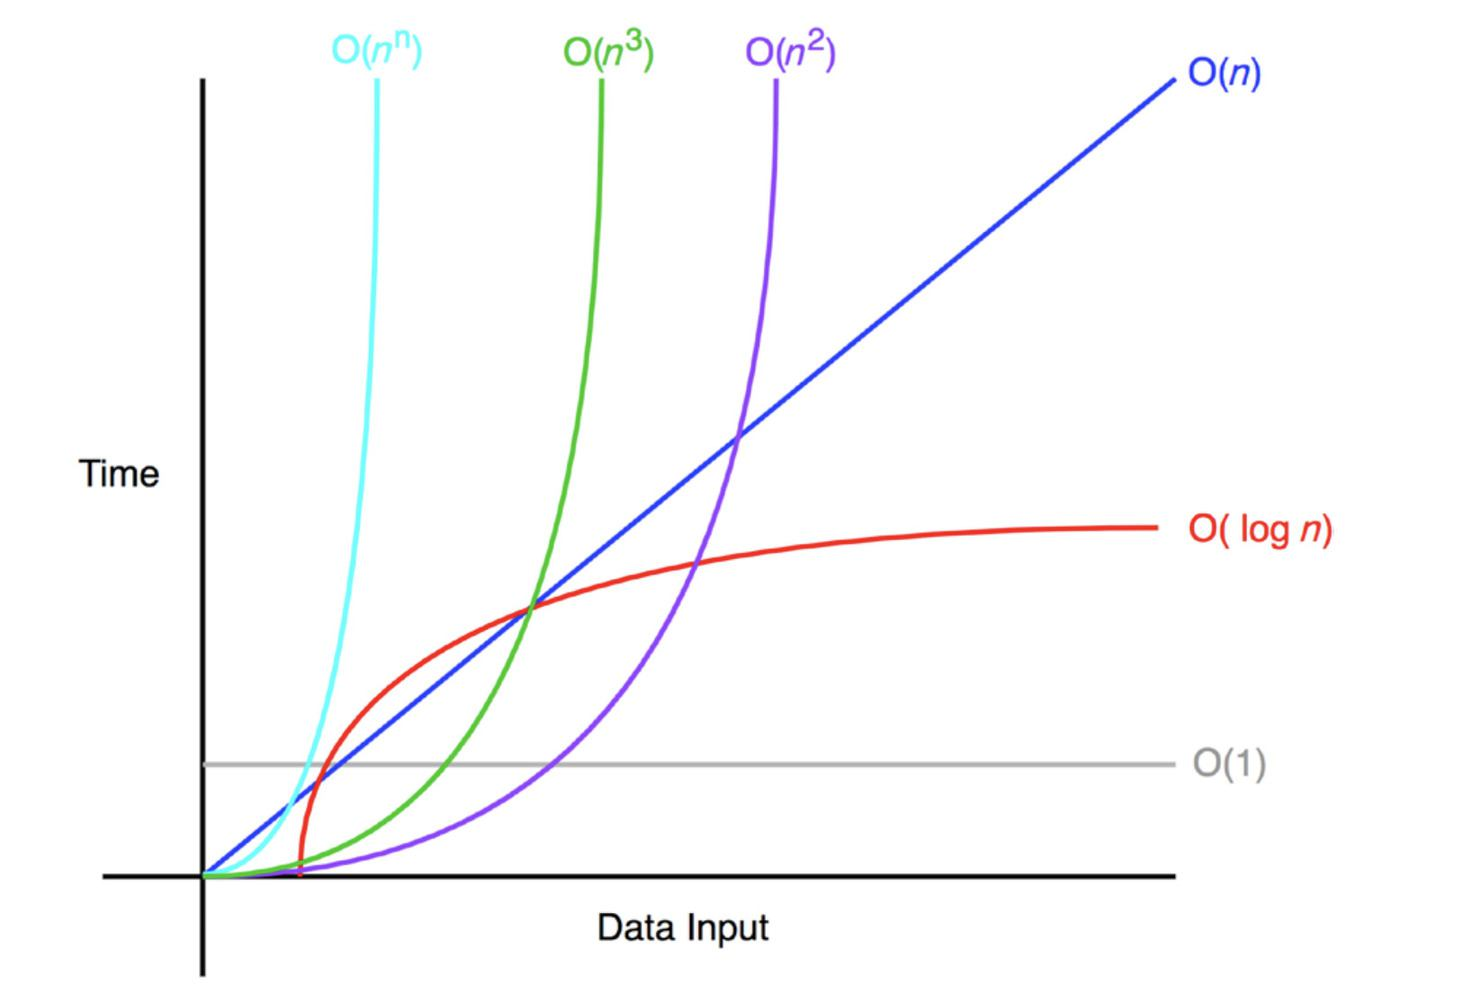
\includegraphics[width=0.3\textwidth]{Pictures/big-o-notation.jpg}
        \caption{Wachstum verschiedener Funktionen}
        \label{fig: WachstumBigO}
    \end{figure}
    Die graphische Darstellung der Funktionen im Bild (\ref{fig: WachstumBigO}) zeigt uns leider nur sechs Funktionen. 
    Um möglichst viele Funktionen in aufsteigendem, asymptotischen Wachstum zu sehen, folgende Abbildung:

    $\mathcal{O}(1) \in [\mathcal{O}(\frac{1}{n^2}) \in \mathcal{O}(\frac{1}{n}) \in \ ] \  \mathcal{O}(\log \log n)\in \mathcal{O}(\log n) \in \mathcal{O}(\sqrt{n}) \in \mathcal{O}(n) \in \mathcal{O}(n\log n) \in [\mathcal{O}({n^c}) \in \mathcal{O}(c^n) \in \ ] \mathcal{O}(n^2) \in \mathcal{O}(2^n) \in \mathcal{O}(2^{n^{2}}) \in \mathcal{O}(n!) $

\newpage
\subsection{Erster Algorithmus} 
    \subsubsection{Maximum Subarray Sum}\label{MSS-Abschnitt}
    Für einen ersten Algorithmus schauen wir den \texttt{Maximum Subarray Sum} Algorithmus an. Dieser Algorithmus enthält ein Array von $n$ rationalen Zahlen $a_1,..., a_n$ und gesucht ist ein Teilstück mit maximaler Summe.  \\
    \textbf{Beispiel}: \\
    Sei ein Array [-2, -5, 6, -2, -3, 1, 5, -6] gegeben, so ist die maximale Teilsumme dieses Array 7, nämlich $ 6 + (-2) + (-3) + 1 + 5 = 7$. \\
      
\begin{algorithm}
    \caption{Maximum Subarray Sum $(a_1,..., a_n)$}
    \label{alg:MSS-1}
    \begin{algorithmic}[1]
    \Function{FindMSS}{Array [$1...n$]}
    \State $S_0 \gets 0$ 
    \For{$i \gets 1,...,n$}
        \State $S_i \gets S_{i-1} + a_i$ 
    \EndFor
    \State maxS $\gets 0$
    \For{$i \gets 1,...,n$}
        \For{$j \gets 1,...,n$}
            \State $S \gets S_j - S_{j-1}$ 
           \State Merke maximales S
        \EndFor
    \EndFor
    \EndFunction

    \end{algorithmic}
    
\end{algorithm}

Dieser naive Algorithmus führt insgesamt $\Theta(n^3)$ viele Additionen aus, was sehr schlecht ist für unseren Algorithmus.

\begin{algorithm}
 \caption{MSS divide and conquer $(a_1,..., a_n)$}
 \label{alg:MSS-Div}
 \begin{algorithmic}[1]
    \Function{MSSDivAndConquer}{Array [$1,...,n$]}
      \State Wenn $n=1$ ist, dann gib $max{a_1,0}$ zurück.
      \State Wenn $n>1$ ist:
      \State Teile die Eingabe in $A_1 = \langle a_1,...,a_{n/2} \rangle$ und $A_2 = \langle a_{n/2+1},...,a_{n} \rangle$ auf
      \State Berechne rekursiv den Wert $W_1$ einer besten Lösung für das Array $A_1$
      \State Berechne rekursiv den Wert $W_2$ einer besten Lösung für das Array $A_2$
      \State Berechne grösste Suffixsumme $S$ in $A_1$
      \State Berechne grösste Suffixsumme $P$ in $A_2$
      \State Setzte $W_3 \gets S+P$
      \State Gib max$\{W_1, W_2, W_3\}$ zurück
    \EndFunction
 \end{algorithmic}
\end{algorithm}

    Wir haben schon eine Verbesserung des Algorithmus von $\Theta(n^3)$ vielen Additionen zu $\Theta(n\log n)$ vielen Additionen. In einem letzten Schritt können wir diesen sogar noch einmal verbessern nämlich bis zu $\Theta(n)$ viele Additionen.

\begin{algorithm}
 \caption{MSS-Induktiv $(a_1,..., a_n)$}
 \label{alg:MSS-Induktiv}
    \begin{algorithmic}[1]
    \Function{MSSInduktiv}{Array [$1,...,n$]}
    \State $randmax \gets 0$
    \State $maxS \gets 0$
        \For{$i \gets 1,...,n$}
            \State $randmax \gets randmax + a_i$
            \If{$randmax > maxS$}
                \State $maxS \gets randmax$
            \EndIf
            \If{$randmax < 0$}
                \State $randmax \gets 0$
            \EndIf
        \State Gib $maxS$ zurück
        \EndFor
    \EndFunction
    \end{algorithmic}
\end{algorithm}

\newpage
%%Chapter 03
\section{Suchen und Sortieren}
\subsection{Suchen}
    In diesem Abschnitt schauen wir wie schnell wir in abstrakten Daten Strukturen suchen, einfügen und löschen können. Die meist gebrauchten Datenstrukturen sind somit in folgender Tabelle aufgeführt mit ihrer korrespondierender Laufzeit: \\
\begin{center}      
\begin{tabular} {|c|c|c|c|}
  \hline
  \label{Tab: LaufzeitenSuchSortier}
  \bfseries Data structure & \bfseries Search & \bfseries Insert & \bfseries Delete\\
  \hline
  Unsorted Array	&$O(n)$				&$O(1)$			&$O(n)$\\
  Sorted Array		&$O(\log{n})$	          	&$O(n)$			&$O(n)$\\
  Unsorted List 	&$O(n)$				&$O(1)$			&$O(n)$\\	
  Sorted List		&$O(n)$				&$O(n)$			&$O(n)$\\	
  Unbalanced Tree	&$O(n)$				&$O(n)$			&$O(n)$\\
  AVL tree		&$O(\log{n})$	        	&$O(\log{n})$	        &$O(\log{n})$\\
  \hline
\end{tabular}
\end{center}  
Wir stellen fest, dass es im Allgemeinen einen Kompromiss gibt zwischen einfachen Datenstrukturen, die ein einfaches Einfügen und Löschen ermöglichen, aber die Einträge nicht vorverarbeiten, um spätere Suchvorgänge zu erleichtern (ungeordnetes Array), und komplexeren Datenstrukturen mit höheren Einfüge- und Löschkosten, die effizienter abgefragt werden können.

\subsubsection{Binary Search} \label{BinarySearch}
    Binary Search ist der standart Suchalgorithmus für \textbf{sortierte} Arrays, da es einen effizienten, logarithmische Laufzeitkomplexität hat.

\begin{algorithm}
\caption{Binary search} 
\label{alg:BinarySearch}
\begin{algorithmic}[1] 
  \Function{FindIndex}{$A$, $e$} \Comment{Search item $e$ in sorted array $A$}
  \State $l, r \gets 0, A\texttt{.length}-1$
  \While{$r > l$}
  \State $m \gets \left\lfloor \frac{l+r}{2} \right\rfloor$
  \If{$A\left[m\right] = e$}
  \State \Return $m$
  \ElsIf{$A\left[m\right] > e$}
  \State $r \gets m-1$
  \Else
  \State $l \gets m+1$
  \EndIf
  \EndWhile
  \State \Return \texttt{"not found"}
  \EndFunction
\end{algorithmic}
\end{algorithm}
Obwohl bei der binären Suche die Kosten für die Suche in geordneten Arrays logarithmisch werden, sind Einfügung und Löschung immer noch linear: im schlimmsten Fall, d.h. wenn das einzufügende oder zu löschende Element das erste Element des Arrays ist, müssen wir alle Elemente um einen Schritt nach rechts/links verschieben.

\subsubsection{Heaps}
Noch effizienter als geordnete Arrays sind daher baumartige Strukturen, bei denen die Kosten für das Einfügen und Löschen ebenfalls logarithmisch sein können. Heaps sind eine spezielle Klasse von baumbasierten Strukturen, die eine effiziente (zeitkonstante) Methode zur Extraktion des kleinsten oder größten Elements bieten.

Genauer gesagt sind Min- (bzw. Max-) Heaps baumbasierte Datenstrukturen, die die folgende Heap-Invariante erfüllen: Wenn $A$ das Elternteil von $B$ ist, dann ist der Wert von Knoten $A$ kleiner (bzw. größer) als der Wert von Knoten $B$. Wir betrachten hier binäre Min-Heaps, was bedeutet, dass ein Elternteil einen kleineren Wert hat als seine (höchstens zwei) Kinder. Für binäre Min-Haufen gilt zusätzlich die folgende Forminvariante: Der betrachtete Haufen ist immer ein vollständiger binärer Baum, d. h. alle Schichten des Baums sind von oben nach unten und von links nach rechts gefüllt.


\begin{figure}[h] 
\caption{Beispiel eines Min- und Max- Heaps}
\centering
\label{fig: Min/Max-heap}
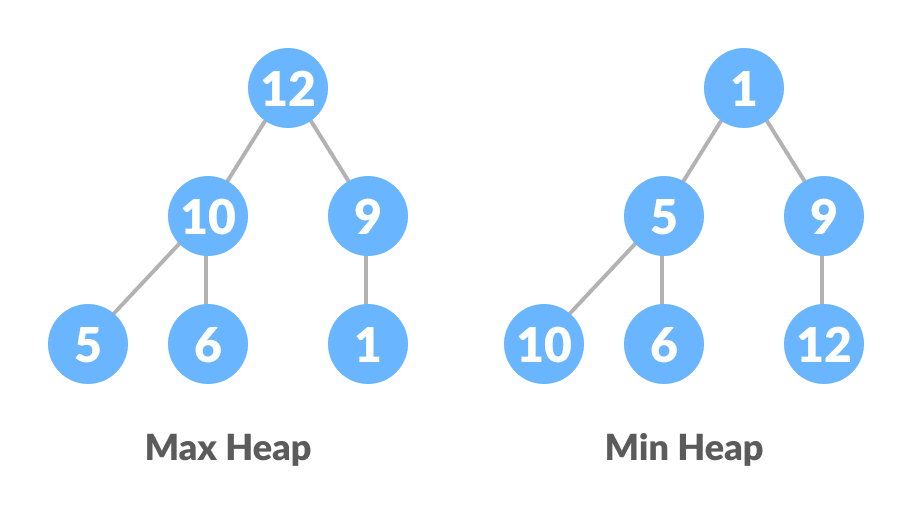
\includegraphics[scale= 0.7]{Pictures/max-heap-min-heap.png}
\end{figure}

\begin{figure}[h] 
\caption{Beispiel 0-Heaps}
\centering
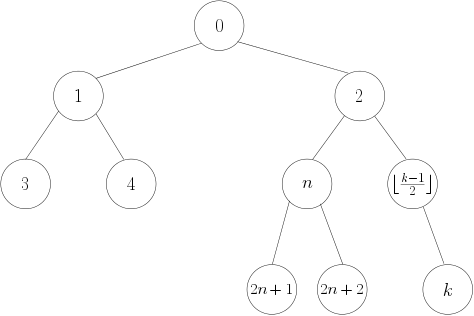
\includegraphics[scale= 0.5]{Pictures/0-heap.png}
\label{fig: 0-Heap}
\end{figure}



\subsubsection*{Implementation}
Die gebräuchlichste Implementierung ist ein Array (mit fester oder dynamischer Größe). Geht man von einem 0-basierten Array aus (vgl. Figure \ref{fig: 0-Heap}), so sind die \textit{children} des Knotens $n$, $2n+1$ und $2n+2$ und die \textit{parent} des Knotens $k$ ist der Knoten $\lfloor \frac{k-1}{2}\rfloor$.

\newpage
\subsubsection*{Common operations} \label{common operations}
Here are the most common operations that a min-heap must support:
\begin{itemize}
\item \textbf{Basic operations}
  \begin{itemize}
  \item Find min,
  \item Delete min,
  \item Insert,
  \item Find min and delete it (pop);
  \end{itemize}
\item \textbf{Initialization}
  \begin{itemize}
  \item Create empty heap,
  \item Heapify (transform array into heap);
  \end{itemize}
\item\textbf{Inspection}
  \begin{itemize}
  \item Return size,
  \item Test if empty;
  \end{itemize}
\item \textbf{Other}
  \begin{itemize}
  \item Increase/decrease,
  \item Delete,
  \item Restore heap invariant,
  \item Merge/union.
  \end{itemize}
\end{itemize}


\subsubsection*{Preserving the heap invariant}
Die Heap Invariante sagt uns eigentlich aus: 
\begin{quote}
    "Das Label jedes Knoten $n$ ist kleiner oder gleich den Labels der Kinder von $n$."
\end{quote}
Bei der Aktualisierung eines Heaps ist es wichtig, die oben beschriebene Invariante beizubehalten. Nach einer Löschung oder einer Einfügung kann es vorkommen, dass ein (einzelnes) Element kleiner wird als eines seiner Kinder; wir können dann die Heap-Invariante in logarithmischer Zeit wiederherstellen, indem wir dieses Element nach unten durchsickern lassen. (Vgl. Durchsickeralgorithmus \ref{alg:DurchsickernHeap})

\begin{algorithm}
\caption{Restore heap invariant by percolating element down} 
\label{alg:DurchsickernHeap}
\begin{algorithmic}[1] 
  \Function{PercolateDown}{$H$, $i$} \Comment{Percolate element $i$ in $H$}
  \State $e \gets H\left[i\right]$
  \If{$2i+2 = H\texttt{.length}$}
  \If{$e > H\left[2i+1\right]$}
  \State Swap $H\left[i\right]$ and $H\left[2i+1\right]$
  \EndIf
  \ElsIf{$2i+2 < H\texttt{.length}$}
  \State $l, r \gets H\left[2i+1\right], H\left[2i+2\right]$
  \If{$l < r$}
  \If{$l < e$}
  \State Swap $H\left[i\right]$ and $H\left[2i+1\right]$
  \State \textsc{PercolateDown}$\left(H, 2i+1\right)$
  \EndIf
  \Else
  \If{$r < e$}
  \State Swap $H\left[i\right]$ and $H\left[2i+2\right]$
  \State \textsc{PercolateDown}$\left(H, 2i+2\right)$
  \EndIf
  \EndIf
  \EndIf  
  \EndFunction
\end{algorithmic}
\end{algorithm}

\subsubsection*{Costs}

In der folgenden Tabelle sind die Kosten von Standard-Heap-Operationen für drei Arten von Heaps zusammengefasst: binäre Heaps, binomische Heaps und Fibonacci-Heaps. \\

\begin{tabular}{|c|c|c|c|}
  \hline
  \label{Tab: KostenHeaps}
\textbf{Operation}    & \textbf{Binary}             & \textbf{Binomial}         & \textbf{Fibonacci}   \\
\hline
search min   & $\Theta(1)$        & $\Theta(1)$      & $\Theta(1)$ \\
delete min   & $\Theta(\log n)$   & $\Theta(\log n)$ & $O(\log n)$ \\
insert       & $\Theta(\log n)$   & $\Theta(1)$      & $\Theta(1)$ \\
increase key & $\Theta(\log n)$   & $\Theta(\log n)$ & $\Theta(1)$ \\
  union        & $\Theta(m \log n)$ & $O(\log n)$      & $\Theta(1)$  \\
                                                         \hline
\end{tabular}


\subsubsection*{Zusammenfassung- Youtube}
\href{https://www.youtube.com/watch?v=0wPlzMU-k00}{Kurze Zusammenfassung anschauen}

\subsection{Binärer Suchbaum}
\subsubsection{Begrifflichkeiten}
Bäume im Allgemeinen gehören zu den wichtigsten in der Informatik auftretenden Datenstrukturen. Seien es Entscheidungsbäume, Syntaxbäume, Ableitungsbäume, Kodebäume oder auch Suchbäume. Bäume sind Listenstrukturen, ein Element referenziert einen \textbf{Knoten}. Jegliche Nachfahren die einen Knoten beinhalten nennt man \textbf{Kinder-Knoten}. Die \textbf{Wurzel} des Baumes ist, von welchem der Baum aus startet. Zusätzlich gilt, dass von jeder Wurzel der verschiedenen Knoten eines Baumes durch genau einen Pfad mit der Wurzel verbunden. Ein \textbf{Blatt} oder \textbf{Blätter} eines Baumes sind die Knoten welche keine Nachfolger haben. Im Beispiel von \ref{fig: binarytree} wären die Blätter dieses Baumes: [3, 7, 13, 18, 23]. Man nennt einen Baum \textbf{geordnet} wenn unter den Kinderknoten eines jeden Knotens eines Baumes eine \textbf{Anordnung definiert} ist, sodass man vom ersten, zweiten, dritten usw. Kinderknoten eines Knotens sprechen kann, so nennt man den Baum geordnet (Vgl. Figure \ref{fig: binarytree}). Im diesem Beispiel ist zu sehen, dass die definierte Anordnung wie folgt ist: Wenn der Wert eines Knotens kleiner ist als die Wurzel, so wird dieser links platziert, und dann wieder mit dem nächsten Knoten verglichen. Sofern dieser nun grösser ist, wie z.B Knoten 12, wird dieser rechts vom Knoten 5 platziert. \\
Ein weiterer Begriff, der wichtig ist im Kontext mit Bäumen ist die \textbf{Höhe} und \textbf{Tiefe} eines Baumes. Diese beiden Begriffe sind wie folgt definiert: 
\begin{itemize}
    \item $depth(v) = $ distance $v$ to root (along unique path)
    \item $height(T) = max_{v \in V} depth(v) + 1$
\end{itemize}
Man fasst die Knoten eines Baumes gleicher Tiefe zu \textbf{Niveaus} zusammen. Die Knoten auf dem Niveau $i$ sind alle Knoten der Tiefe $i$. Die Höhe des Beispiels (\ref{fig: binarytree}) wäre also der Pfad von $(15-5-12-10-6-7) + 1 = 6 $ und die Tiefe vom Knoten 20 wäre: 2. \\
Zusätzlich gilt: die Tiefe eines binary tree ist gleich wie die Höhe eines binary trees.\footnote{\href{https://www.baeldung.com/cs/binary-tree-height}{weitere Beispiele \& Erklärungen}}
Des weiteren heisst ein Baum \textbf{vollständig} wenn er auf jedem Niveau die maximal mögiche Knotenanzahl hat und sämtliche Blätter dieselbe Tiefe haben. 
Auch wie bei dem Heap gelten die "Basic operations": Einfügen, löschen, suchen eines Elementes und das Traversieren des Baumes (Vgl. \ref{common operations}). 

\begin{figure}[h] 
\caption{Beispiel eines geordneten Binärbaumes}
\centering
\includegraphics[scale= 0.7]{Pictures/Pseudobinärersuchbaum.svg.png}
\label{fig: binarytree}
\end{figure}


\subsubsection{ADT- Wörterbuch}
Wir wollen ein Wörterbuch $W$ welches über 
\begin{enumerate}
    \item \texttt{search}$(x,W)$ : ist \texttt{int} $x$ in $W$?
    \item \texttt{insert}$(x,W)$ : füge \texttt{int} $x$ in $W$ ein
    \item \texttt{delete}$(x,W)$ : lösche \texttt{int} $x$ in $W$
\end{enumerate} verfügt und jedes Element $x$ nur einmal vorkommen darf. Dieses Wörterbuch können wir einfach in einem binärern Suchbaum implementieren, wobei für jeden Knoten $x$ alle Schlüssel im linken Teilbaum $< x$ und alle Schlüssel im rechten Teilbaum $> x$ (Vgl. Figure \ref{fig: binarytree}). Die Laufzeit des Einfügens in den Suchbaum dauert für das \texttt{search}: $\mathcal{O}(h)$, \texttt{insert}: $\mathcal{O}(h)$ und für das \texttt{remove}$(x)$ gilt folgendes:
\begin{itemize}
    \item Fall 1: $x$ hat keine Kinder
    \item Fall 2: $x$ hat genau ein Kind, Parent zum Kind anhängen
    \item Fall 3: $x$ hat zwei Kinder: Wenn wir dens Schlüssel $15$ in Figure: \ref{fig: binarytree} löschen $\implies$ wir nehmen das kleinste Element im rechten Teilbaum, hier Schlüssel $16$, ersetzen diesen mit dem zu löschenden Element und löschen den Schlüssel $16$ an der alten Position. $\mathcal{O}(h)$
\end{itemize}
Problem bei diesen Binärenbäume: $h$ kann sehr gross werden wenn wir z.B 2, 5, 8, 10, 12 ,15 nacheinander einsetzen würden. Um $h = \mathcal{O}(h)$ zu erlangen nutzen wir AVL-Bäume (\ref{AVL-Abschnitt}).

\subsection{AVL-Trees} \label{AVL-Abschnitt}
Ein binärer Suchbaum ist \textit{AVL-ausgegelichen} oder höhenbalanciert. Kurz: Ein AVL Baum, wenn für jeden Knoten $p$ des Baumes gilt, dass sich die Höhe des linken Teilbaumes von der Höhe des rechten Teilbaumes von $p$ um höchstens 1 unterscheidet. In der folgenden Abbildung(\ref{fig: AVL-trees}) ist in (a)  und (c) ein AVL-Baum zu sehen. (b) hingegen ist kein AVL-Baum.\footnote{\href{https://www.cs.usfca.edu/~galles/visualization/AVLtree.html}{Animationen von AVL-Trees}}

\begin{figure}[h] 
\caption{Beispiel von zwei AVL-Bäume}
\centering
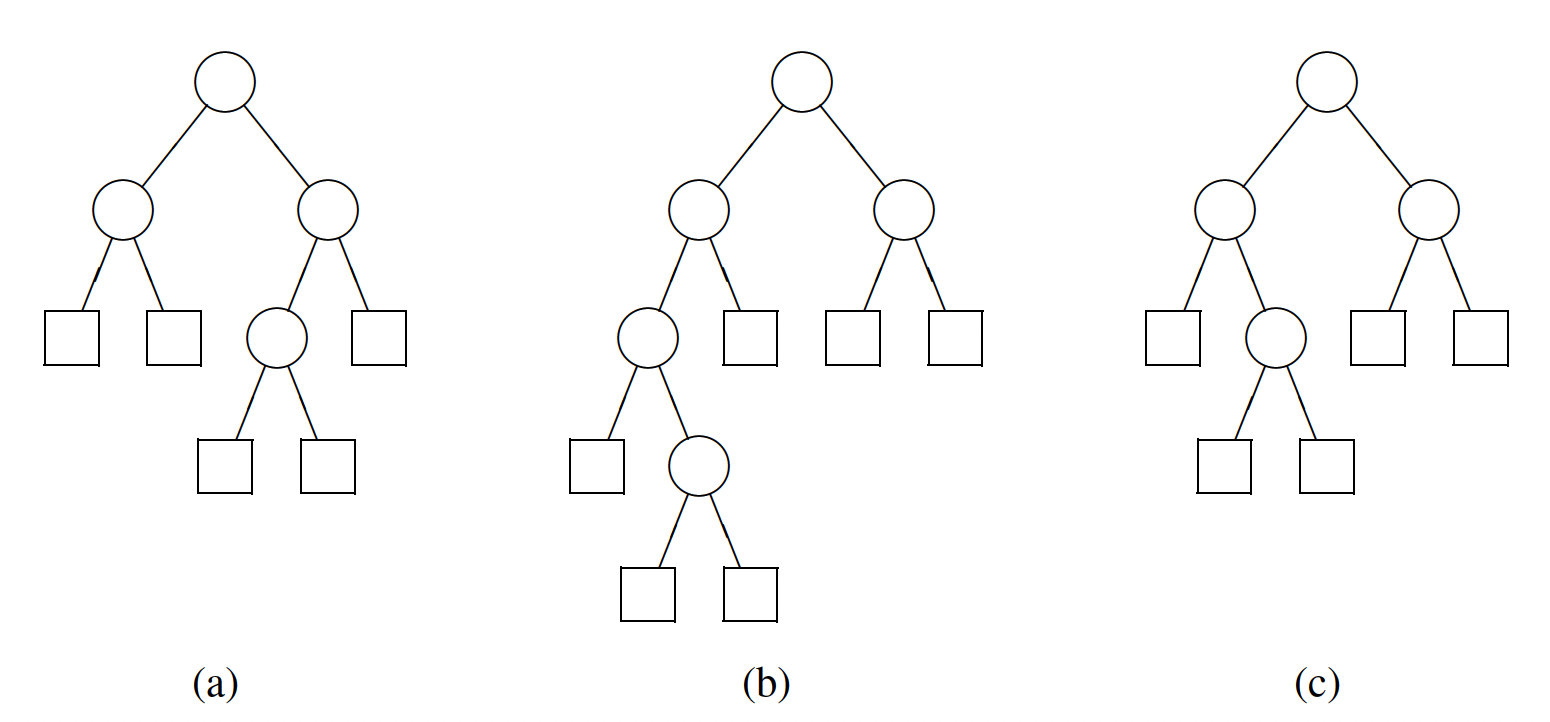
\includegraphics[scale= 0.5]{Pictures/AVL-trees.png}
\label{fig: AVL-trees}
\end{figure}

AVL-Bäume mit $N$ inneren Knoten und $N+1$ Blättern haben eine höhe von $\mathcal{O}(\log N)$. Man überlegt sich was die minimale Blatt-und Knotenzahl eines AVL-Baumes gegebener Höhe $h$ ist. Es gilt: AVL-Baum der Höhe 1 hat 2 Blätter und ein AVL-Baum der Höhe 2 mit minimaler Blattzahl hat 3 Blätter (Vgl. Figure \ref{fig: AVL-trees-height}). Ein AVL-Baum der Höhe $h+2$ mit minimaler Blattzahl erhält man, wenn man je einen AVL-Baum mit der Höhe $h+1$ und $h$ mit minimaler Blattzahl wie in Figure (\ref{fig: AVL-trees-allg}) zu einem Baum der Höhe $h+2$ zusammenfügt.

\begin{figure}[h] 
\caption{AVL-Baum mit Höhe 1 und 2}
\centering
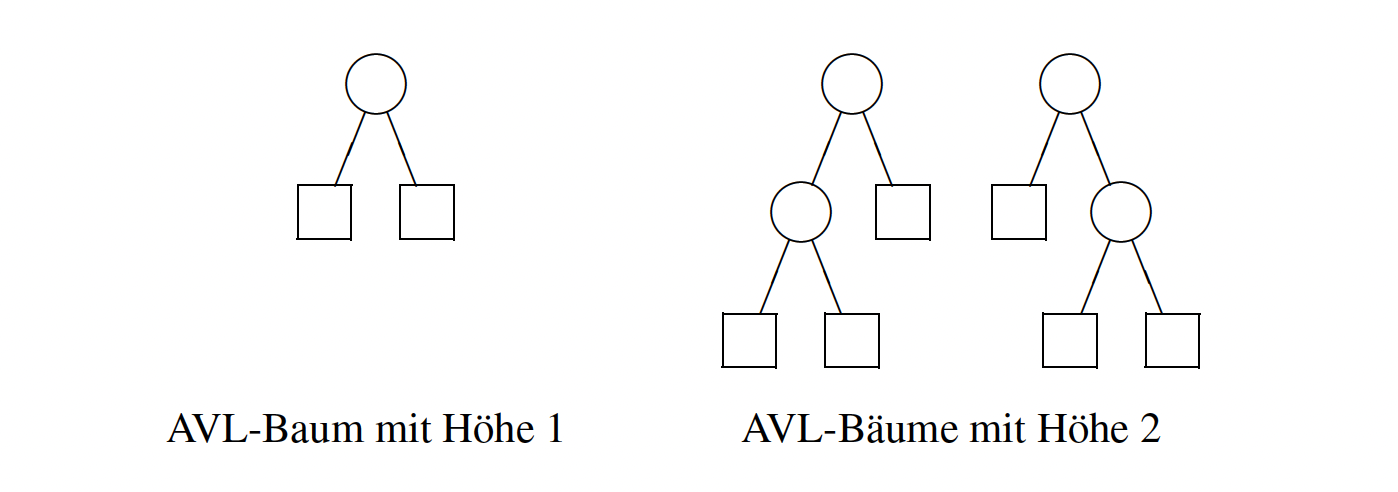
\includegraphics[width = 0.6\textwidth]{Pictures/AVL-trees-height.png}
\label{fig: AVL-trees-height}
\end{figure}

\begin{figure}[t] 
\caption{AVL-Baum}
\centering
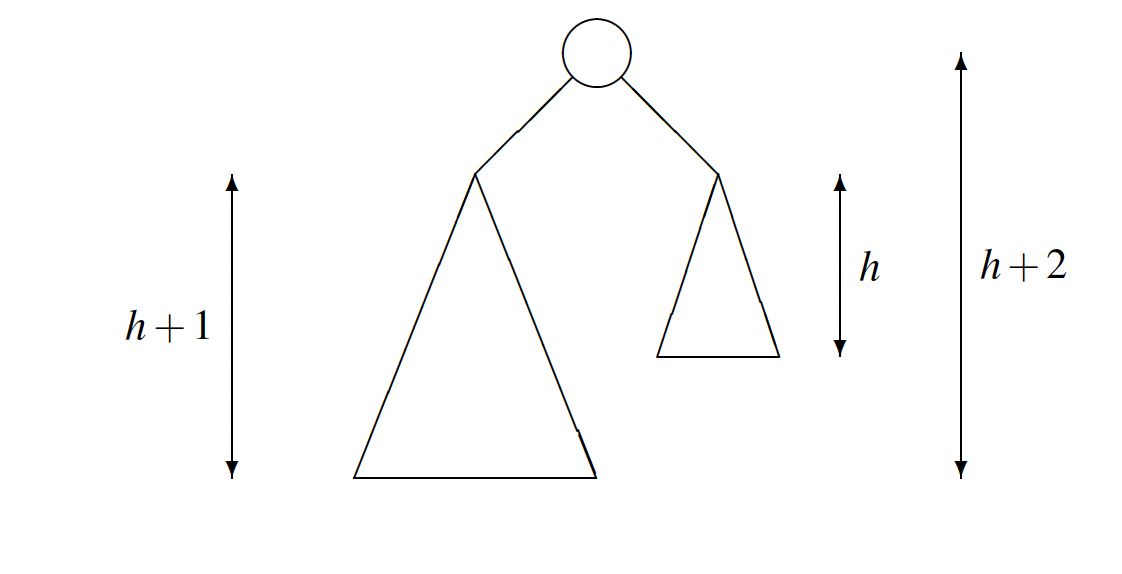
\includegraphics[width = 0.8\textwidth]{Pictures/AVL-trees-allg.png}
\label{fig: AVL-trees-allg}
\end{figure}

\newpage
\subsubsection{Suchen, Einfügen und Entfernen in AVL-Bäumen}
Da AVL-Bäume eigentlich binäre Suchbäume sind, kann man ihnen nach einem Schlüssel genauso suchen wie in einem natürlichen Baum. Im schlechtesten Fall ist die Suche nach einem Schlüssel von Wurzel bis zu einem Blatt. Da die Höhe logarithmisch beschränkt ist, wird dies im worst case $\mathcal{O} (\log N)$ Schritte benötigen, wobei der worst case in einem normalen binären Suchbaum $\mathcal{O} (N)$ ist (alle links oder rechts an der Wurzel). Die AVL-Bäume brauchen genau $\Theta (n)$ Speicher. Sie verfügen über die Standartoperationen von Suchen, Einfügen und Entfernen, die eine Komplexität von $\mathcal{O}(\log n)$ haben. 

\subsubsection{Einfügen}\label{subsection EinfügenAVL}
Damit der Schlüssel eingefügt werden kann, überprüfen wir in einem ersten Schritt nach dem Schlüssel im Baum. Wenn dieser Schlüssel bereits vorhanden ist, endet der Vorgang. Sofern dieser aber nicht in dem Baum ist fügen wird diesen ein wie bei einem normalen Baum.

Das Problem welches wir nun erhalten ist die Aufrechterhaltung der AVL-Eigenschaft. Wenn wir bei Figure (\ref{fig: AVL-ausgangslage}) den Key 5 einfügen wollen, wird im nächsten Schritt Figure (\ref{fig:AVL-verletzt}) die Bedingung verletzt, da die Höhen des linken und rechten Teilbaumes sich um mehr als 1 unterscheiden. Man muss also die AVL-Ausgeglichenheit wieder herstellen. Dazu läuft man von der Einfügestelle den Suchpfad entlang zur Wurzel zurück und prüft an jedem Knoten (Vgl. Equation: (\ref{eqn: bal(p)}), ob die Höhendifferenz  zwischen linkem und rechtem Teilbaum noch innerhalb der vorgeschriebenen Grenzen liegt. Ist das nicht der Fall, führt man eine so genannte Rotation oder eine Doppelrotation durch (Vgl. \ref{Rotationsabschnitt}), die die Sortierung der Schlüssel nicht beeinflusst, aber die Höhendifferenzen in den richtigen Bereich bringt.
 Es genügt, an jedem inneren Knoten $p$ den so genannten \textbf{Balancefaktor} $bal(p)$ mitzuführen, der wie folgt definiert ist:
\begin{equation} \label{eqn: bal(p)}
    bal(p) = \text{Höhe des rechten Teilbaumes von } p - \text{Höhe des linken Teilbaumes von } p
\end{equation}
AVL-Bäume sind offenbar gerade dadurch charakterisiert, dass für jeden inneren Knoten $p$ gilt: $bal(p) \in \{ -1, 0, +1\}$. Die drei Fälle sind in Figure \ref{fig: bal(p) für alle} abgebildet.


\begin{figure}[h] 
   \centering
     \begin{subfigure}[h]{0.5\textwidth}
         \centering
         \includegraphics[width = 0.45\textwidth]{Pictures/AVL-einfügen1.png}
         \caption{Ausgangslage}
         \label{fig: AVL-ausgangslage}
     \end{subfigure}
     \hfill
     \begin{subfigure}[h]{0.45\textwidth}
         \centering
         \includegraphics[width = 0.45\textwidth]{Pictures/AVL.einfügen2.png}         \caption{AVL-Bedingung verletzt}
         \label{fig:AVL-verletzt}
     \end{subfigure}
     \caption{Wie die AVL-Eigenschaft verletzt werden kann}
    \label{fig: AVL-ausgangslage-verletzt}
\end{figure}


\begin{figure}[h!]
\centering
\begin{subfigure}{0.6\textwidth}
    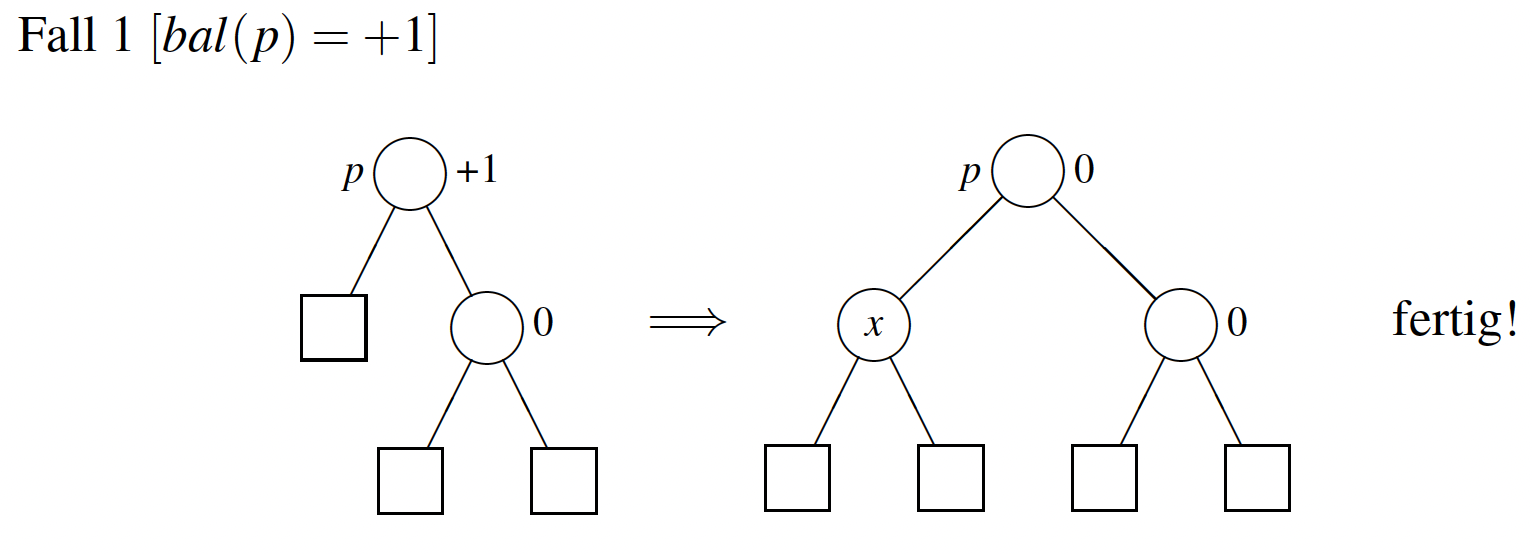
\includegraphics[width=\textwidth]{Pictures/AVL-bal(+1).png}
        \caption{$bal(p) = +1$}
        \label{fig: bal(p) = +1}
\end{subfigure}
\hfill
\begin{subfigure}{0.6\textwidth}
    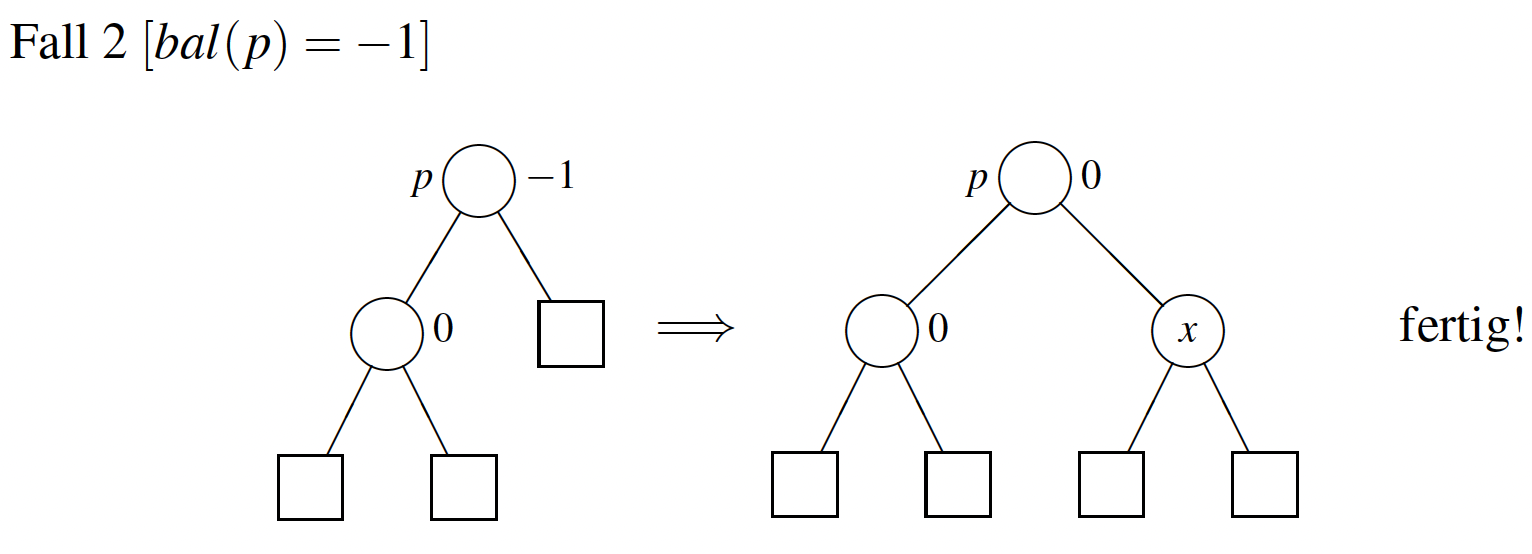
\includegraphics[width=0.8\textwidth]{Pictures/AVL-bal(-1).png}
        \caption{$bal(p) = -1$}
        \label{fig: bal(p) = -1}
\end{subfigure}

\begin{subfigure}{0.6\textwidth}
    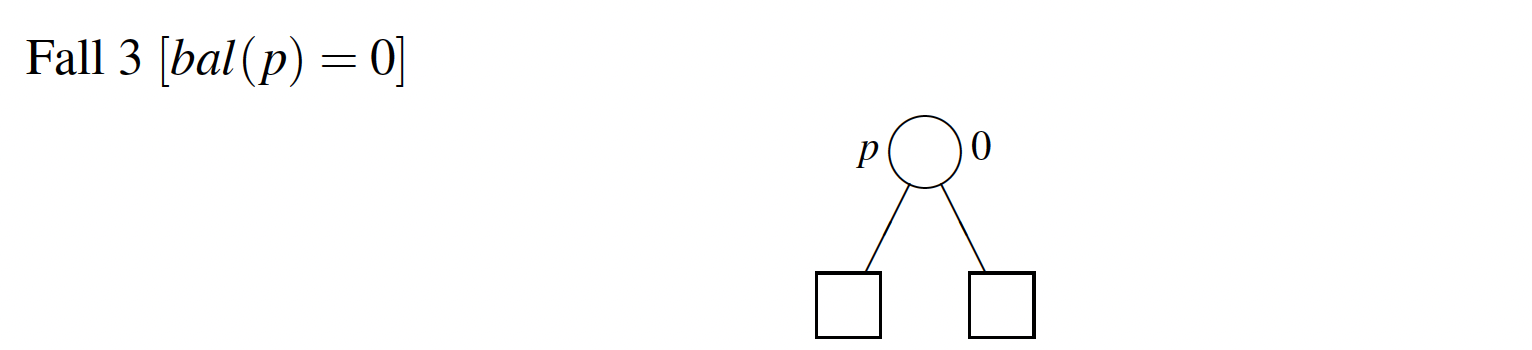
\includegraphics[width=0.8\textwidth]{Pictures/AVL-bal(0).png}
        \caption{$bal(p) = 0$}
        \label{fig: bal(p) = 0}
\end{subfigure}
        
\caption{Veranschaulichung von $bal(p) \in \{-1, 0, +1\}$ und dessen Balancierung}
\label{fig: bal(p) für alle}
\end{figure}

\subsubsection{Entfernen}\label{subsection EntfernenAVL}
Wie beim Einfügen in den AVL-Tree gehen wir zuerst so vor wie in natürlichen Suchbäumen. Man sucht den zu entfernenden Schlüssel, findet man diesen nicht, so ist das Entfernen beendet. Falls dies nicht der Fall ist, haben wir drei Fälle der Entfernung, die auch mithilfe des Balancefaktors $bal(p)$ (Vgl. \ref{eqn: bal(p)}) analysiert werden können. Eine detailliertere Ansicht über das Entfernen in Abschnitt \ref{AVL-Trees-Anhang}.



\subsubsection{Rotationen} \label{Rotationsabschnitt}
In den vorherigen Abschnitten (\ref{subsection EinfügenAVL}, \ref{subsection EntfernenAVL}) haben wir bereits \textbf{Rotationen} gesehen. Wir unterscheiden insgesamt 4 Fälle: LR, RL, LL, RR. \\
LL und RR müssen jeweils nur eine Operation durchführen, wohingegen LR und RL zwei Operationen durchführen müssen. 

\begin{figure}[h]
    \centering
    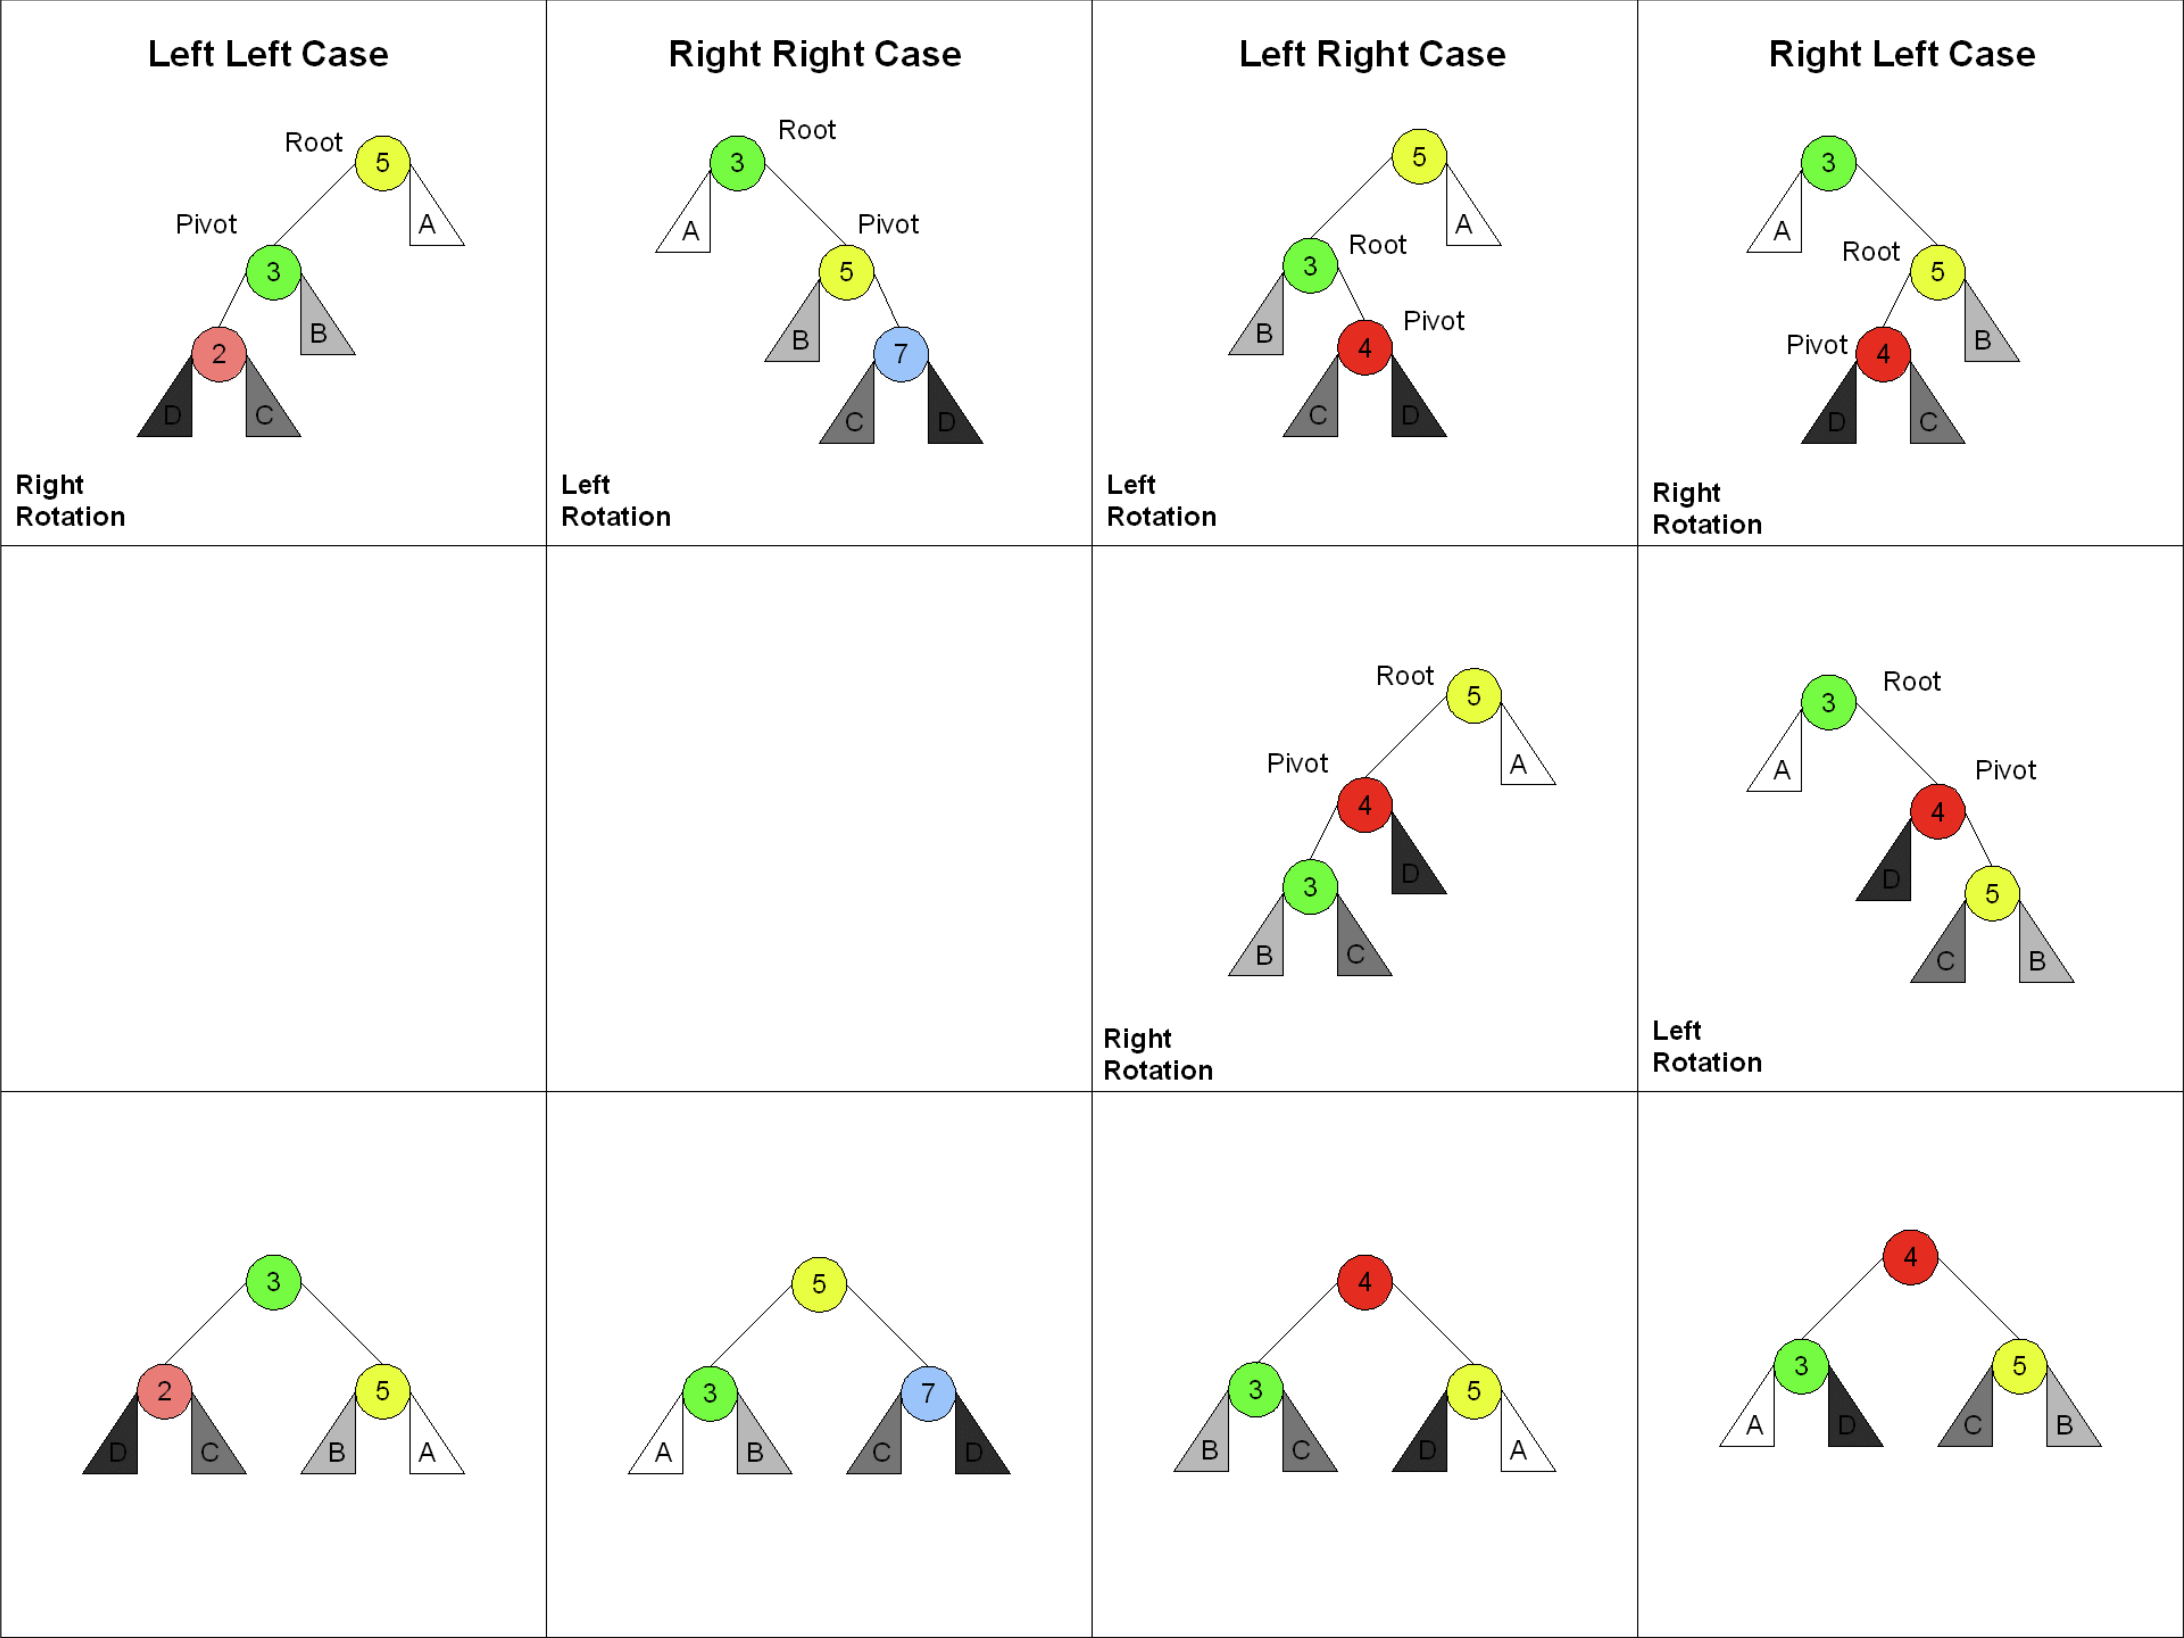
\includegraphics[width = \textwidth]{Pictures/AVL-Rotations.png}
    \caption{Alle Fälle zum AVL-Tree zu balancieren}
    \label{fig:AVL-rotations}
\end{figure}


\newpage
\subsection{Sortier-Algorithmen}
Zunächst wollen wir das Sortierproblem genauer fixieren: Wir nehmen an, es sei eine
Menge von Sätzen gegeben; jeder Satz besitzt einen Schlüssel. Zwischen Schlüsseln ist
eine Ordnungsrelation „<" oder „$\leq$" erklärt. Ausser der Schlüsselkomponente können
Sätze weitere Komponenten als „eigentliche“ Information enthalten. Im Allgemeinen gilt, dass nicht schneller als $\Omega(n\log n)$ sortiert werden kann, da folgendes gilt: $2^{h+1} \geq \#Vertices \geq \#$possible Outputs $= n!$, wobei $h$ die Tiefe rsp \# Vergleiche eines Binärbaumes darstellt.

\begin{equation*}
    \implies 2^{h+1} \geq \#Vertices \geq n! \\
    \implies h \geq \log_2(n!) -1 \geq \Omega(n\log n)
\end{equation*}


\subsubsection{Eigenschaften von Sortier-Algorithmen}

\paragraph{Stability} Zwei Objekte mit gleichen Schlüsseln erscheinen in der (sortierten) Ausgabe in der gleichen Reihenfolge, wie sie in der Eingabe erschienen.
\paragraph{In-place} oder in-situ beschreiben jene Algorithmen, die die Eingabe ohne zusätzliche Datenstruktur und damit ohne zusätzlichen Speicherplatz umwandeln. In einigen Fällen ist zusätzlicher Speicherplatz zur Speicherung einiger Variablen zulässig.

\begin{table}[H]
\centering
\caption{Properties of sorting algorithms}
\label{my-label}
~\\
\begin{tabular}{|r|c|c|c|c|c|c|@{}}
  \cline{2-7}
  \multicolumn{1}{c|}{} & \textbf{bubble} & \textbf{insert} & \textbf{select} & \textbf{quick} & \textbf{merge} & \textbf{heap} \\
        \hline
stable  & Yes      & Yes      & No      & No     & Yes     & No    \\
  in-situ & Yes      & Yes      & Yes      & Yes     & No     & Yes   \\
  \hline
\end{tabular}
\end{table}


\subsubsection{Bogo sort}
Bogo sort $\mathcal{O}(n\cdot n!)$ - This is a fairly inefficient sorting algorithm that generates a random permutation until the elements are sorted. An analogy with a deck of card would be to shuffle the deck, then check if it is sorted and loop if it is not. 


\begin{algorithm}
    \caption{Bogo Sort}
    \label{alg:BogoSort}
    \begin{algorithmic}
        \While{$\neg \textsc{isSorted}\left(A\right)$}
        \State $A \gets \textsc{randomPermutation}\left(A\right)$
        \EndWhile
    \end{algorithmic}
\end{algorithm}
This algorithm doesn't have a worst case asymptotic time as it is not guaranteed to terminate within a given time. 



    \subsubsection{Bubblesort}\label{Bubblesort}
    Bubblesort $\mathcal{O}(n^2)$ - ist ein Verfahren, welches nach dem Motto \textit{Sortierten durch Einfügen} leben. Bubblesort ist ein Sortierverfahren, das solange zwei jeweils
    benachbarte, nicht in der richtigen Reihenfolge stehende Elemente vertauscht, bis keine Vertauschungen mehr nötig sind.
    Um ein genaueres Verständnis zu erlangen ein Beispiel: \\
    
\begin{algorithm}
    \caption{Bubble sort}
    \label{alg:BubbleSort}
    \begin{algorithmic} 
        \State $swapped \gets \texttt{true}$
        \While{$swapped$}
        \State $swapped \gets \texttt{false}$
        \For {$i \in \left\lbrace 0, \dots, A\texttt{.length}-1 \right\rbrace$}
        \If{$A\left[i\right]>A\left[i+1\right]$}
        \State Swap $A\left[i\right]$ and $A\left[i+1\right]$
        \State $swapped \gets \texttt{true}$
        \EndIf
        \EndFor
        \EndWhile
    \end{algorithmic}
\end{algorithm}
    \begin{table}[h]
        \centering
        \begin{tabular}{c|c|c|c}
            \textbf{1. (Schritt 6 \& 5)}    & 
            \textbf{2.}    & 
            \textbf{3.}    &
            \textbf{4.}   \\
            
            \hline
            6 5 3 1 8 7 2 4 & 
            \textcolor{red}{3 5} 1 6 7 2 4 8  &
            1 \textcolor{red}{3 5} 6 2 4 7 8 & 
            1 3 \textcolor{red}{2 5} 4 6 7 8 \\
            
            \textcolor{red}  {5 6} 3 1 8 7 2 4 &
            3\textcolor{red} {1 5} 6 7 2 4 8 &
            1 3 \textcolor{red}{5 6} 2 4 7 8 & 
            1 3 2 \textcolor{red}{4 5} 6 7 8 \\
            
            5 \textcolor{red}{3 6} 1 8 7 2 4 &
            3 1 \textcolor{red}{5 6} 7 2 4 8 &
            1 3 5 \textcolor{red}{2 6} 4 7 8 &
            1 3 2 4 \textcolor{red}{5 6} 7 8 \\

            5 3 \textcolor{red}{1 6} 8 7 2 4 & 
            3 1 5 \textcolor{red}{6 7} 2 4 8 &
            1 3 5 2 \textcolor{red}{4 6} 7 8 &
            1 3 2 4 5 \textcolor{red}{6 7} 8 \\

            5 3 1 \textcolor{red}{6 8} 7 2 4 &
            3 1 5 6 \textcolor{red}{2 7} 4 8 &
            1 3 5 2 4 \textcolor{red}{6 7} 8 &
            1 3 2 4 5 6 \textcolor{red}{7 8} \\

            5 3 1 6 \textcolor{red}{7 8} 2 4 &
            3 1 5 6 2 \textcolor{red}{4 7} 8 &
            1 3 5 2 4 6 \textcolor{red}{7 8} &
            \textcolor{red}{1 3} 2 4 5 6 7 8\\

            5 3 1 6 7  \textcolor{red}{2 8} 4 &
            3 1 5 6 2 4  \textcolor{red}{7 8} &
             \textcolor{red}{1 3} 5 2 4 6 7 8 &
            1  \textcolor{red}{2 3} 4 5 6 7 8 \\

            5 3 1 6 7 2 \textcolor{red}{4 8} & 
          \textcolor{red}{1 3} 5 6 2 4 7 8 &
            1 \textcolor{red}{3 5} 2 4 6 7 8 &
            \\
       
        \end{tabular}
        \caption{Tabelle wird von oben nach unten, links nach rechts interpretiert}
        \label{tab:BubblesortTable}
    \end{table}
\newpage
 \subsubsection{InsertionSort}\label{Insertionsort}
    InsertionSort $\mathcal{O}(n^2)$ [worst and average case] - ist ein Algorithmus, der der Art und Weise, wie ein Mensch ein Kartenspiel sortiert, sehr ähnlich ist. Er geht so vor, dass er eine Folge von bereits sortierten Elementen behält und immer das nächste Element in der Folge berücksichtigt. Dieses Element wird dann an der richtigen Stelle in der sortierten Folge eingefügt, wobei alle größeren Elemente nach rechts verschoben werden.

\begin{algorithm}
    \caption{Insertion sort}
    \label{alg:InsertionSort}
    \begin{algorithmic} 
        \For {$i \in \left\lbrace 0, \dots, A\texttt{.length} - 1 \right\rbrace$}
        \State $v \gets A\left[i\right]$
        \State $j \gets i-1$
        
        \While{$j\geq 0$ \textbf{and} $A\left[j\right]>v$}
        \State $A\left[j+1\right] \gets A\left[j\right]$
        \State $j\leftarrow j-1$
        \EndWhile
        
        \State $A\left[j+1\right] \gets v$
        \EndFor
    \end{algorithmic}
\end{algorithm}

    \begin{figure}[h]
        \centering
        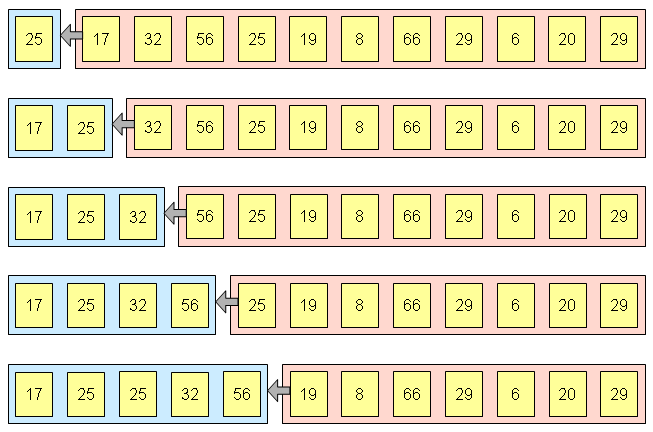
\includegraphics[scale=0.3]{Pictures/insertionsort_version1.png}
        \caption{InsertionSort-Beispiel}
        \label{fig:InsertionSort}
    \end{figure}
    
  \subsubsection{SelectionSort}\label{Selectionsort}
   Selection Sort $\Theta(n^2)$ - Dieser Algorithmus behält ebenfalls eine Folge von sortierten Elementen bei und erweitert sie iterativ um das größte der verbleibenden unsortierten Elemente. Dann tauscht er dieses Element mit demjenigen aus, das den sortierten Elementen am nächsten liegt. Dadurch wird das nächste Element ausgewählt, daher der Name.
 
 \subsubsection*{Complexity}
    Worst case: $\mathcal{O}(n^2)$, Best case: $\mathcal{O}(n^2)$: \\
    $\sum_{i=1}^{n-1} (n-i) = n(n-1)-\sum_{i=1}^{n-1} i = n^2 - n - \frac{n^2-n}{2} = \frac{n^2-n}{2} = \Theta(n^2)$
    

    \begin{algorithm}[h]
        \caption{Selection sort}
        \label{alg:SelectionSort}
        \begin{algorithmic} 
          \For{$i \in \left\lbrace 0, A\texttt{.length}-2 \right\rbrace$}
          \State $m, v \gets i, A\left[i\right]$
          \For {$j \in \left\lbrace i+1, \dots, A\texttt{.length} -1\right\rbrace$}
          \If{$A\left[j\right] < v$}
          \State $m, v \gets j, A\left[j\right]$
          \EndIf
          \EndFor
          \If{$m \neq i$}
          \State Swap $A\left[i\right]$ and $A\left[m\right]$
          \EndIf
        
          \EndFor
        \end{algorithmic}
    \end{algorithm}
    
    \begin{figure}[h]
        \centering
        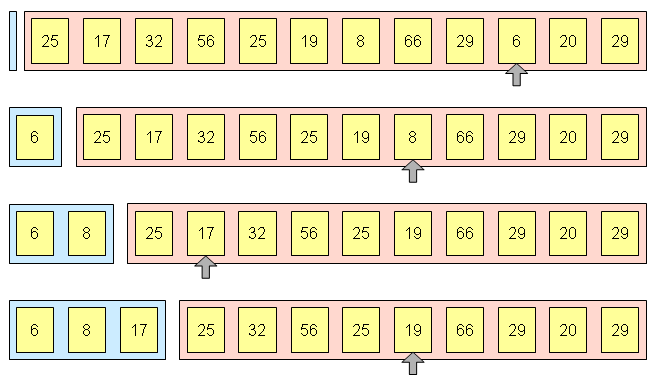
\includegraphics[scale=0.3]{Pictures/selectionsort_idee_version1.png}
        \caption{SelectionSort-Beispiel}
        \label{fig:SelectionSort}
    \end{figure}

   
\newpage    

    \subsubsection{Quicksort}\label{Quicksort}
    Quicksort $\mathcal{O}(n\log n)$ - Dieser Algorithmus funktioniert, indem er rekursiv einen Pivot (ein Element, normalerweise an der ersten oder letzten Position im Array) wählt und alle anderen Elemente in Bezug auf diesen aufteilt. Er erstellt zunächst die Mengen $S^-$ und $S^+$, in denen alle Elemente, die kleiner/größer als der Drehpunkt sind, gespeichert werden. Dann ruft es sich selbst rekursiv auf diesen beiden Mengen auf, und nachdem sie sortiert zurückgegeben wurden, fügt es sie einfach zusammen, wobei es den Drehpunkt in der Mitte hinzufügt. Die Rekursion endet im Basisfall, in dem das Array nur ein Element enthält. Es ist zu beachten, dass auch eine In-Place-Implementierung möglich ist, die den Speicher-Overhead reduziert. Dieser Algorithmus hat eine schlechtere obere Schranke für die Operationszeit, wird aber in der Praxis häufig verwendet, da die durchschnittliche Zeit besser ist als bei Merge und Heap Sort. Beachten Sie, dass der $\cdot$-Operator hier Verkettung bedeutet.

    \begin{algorithm}[h]
        \caption{Quicksort}
        \begin{algorithmic}
            \label{alg:Quicksort}
        \Function{QuickSort}{$A$}
        \If{$A\texttt{.length} \leq 1$}
        \State \Return $A$
        \EndIf
        \State Pick pivot $p \gets A[0]$
        \For{$i \in \left\lbrace 1, \dots, A\texttt{.length}-1 \right\rbrace$}
        \If{$A\left[i\right]\leq p$}
        \State $S^-\texttt{.add}\left(A\left[i\right]\right)$
        \Else
        \State $S^+\texttt{.add}\left(A\left[i\right]\right)$
        \EndIf
        \EndFor
        \State $S^+ \gets \textsc{QuickSort}\left(S^+\right)$
        \State $S^- \gets \textsc{QuickSort}\left(S^-\right)$
        \State \Return $S^- \cdot \left\lbrace p\right\rbrace \cdot S^+$
        \EndFunction
        \end{algorithmic}
        \end{algorithm}

\begin{figure}[h]
    \centering
    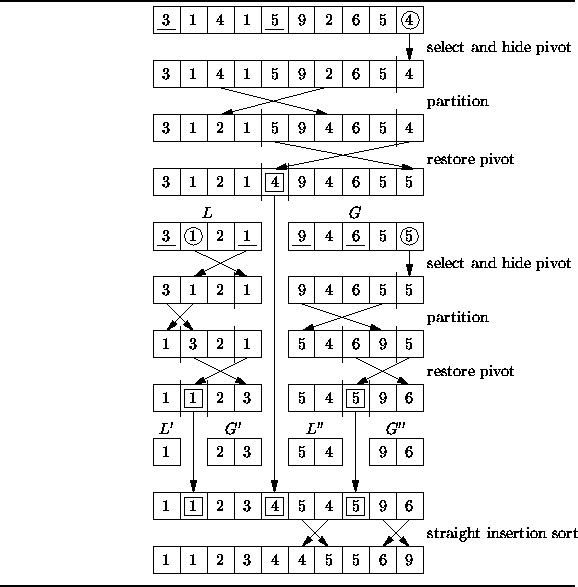
\includegraphics[scale = 0.4]{Pictures/Qcksort.jpeg}
    \caption{Quicksort Algoritihmus}
    \label{fig:QuickSort}
\end{figure}

        
\newpage
    \subsubsection{Mergesort}\label{Mergesort}
        Mergesort $\mathcal{O}(n \log n)$ - Dieser Algorithmus arbeitet ebenfalls rekursiv. Er teilt die Eingabe in zwei Mengen auf und ruft sich dann selbst rekursiv auf diesen Mengen auf. Nachdem die beiden Mengen sortiert zurückgegeben wurden, führt er sie in linearer Zeit zusammen. Der Name leitet sich von diesem letzten Teil des Algorithmus ab. Für detaillierte Ansicht wie der Algorithmus funktioniert (Vgl. Figure \ref{fig:MergeSort2}).        
        \begin{algorithm}[h]
            \caption{Merge sort}
            \label{alg:MergeSort}
            \begin{algorithmic}
              \Function{MergeSort}{$A$}
              \If{$A\texttt{.length} \leq 1$}
              \State \Return $A$
              \EndIf
              \State $n \gets A\texttt{.length}$
              \State $n_1 \gets \frac n2$
              \State $n_2 \gets n-n_1$
              \For{$i \in \left\lbrace 0, \dots, A\texttt{.length} - 1 \right\rbrace$}
              \If{$i < n_1$}
              \State $S^-\texttt{.add}\left(A\left[i\right]\right)$
              \Else
              \State $S^+\texttt{.add}\left(A\left[i\right]\right)$
              \EndIf
              \EndFor
              \State $S^+ \gets \textsc{MergeSort}\left(S^+\right)$
              \State $S^- \gets \textsc{MergeSort}\left(S^-\right)$
              % merge
              \State $i\gets 0$ \Comment{Merge $S^+$ and $S^-$}
              \State $j\gets 0$
              \While{$i<n_1$ \textbf{and} $j<n_2$}
              \If{$S^-\left[i\right]\leq S^+\left[j\right]$}
              \State $R\texttt{.add}\left(S^-\left[i\right]\right)$
              \State $i \gets i+1$
              \Else
              \State $R\texttt{.add}\left(S^+\left[j\right]\right)$
              \State $j \gets j+1$
              \EndIf
              \EndWhile
              \State Concatenate remaining elements to $R$
              \State \Return $R$
              \EndFunction
            \end{algorithmic}
            \end{algorithm}

    \begin{figure}[h]
        \centering
        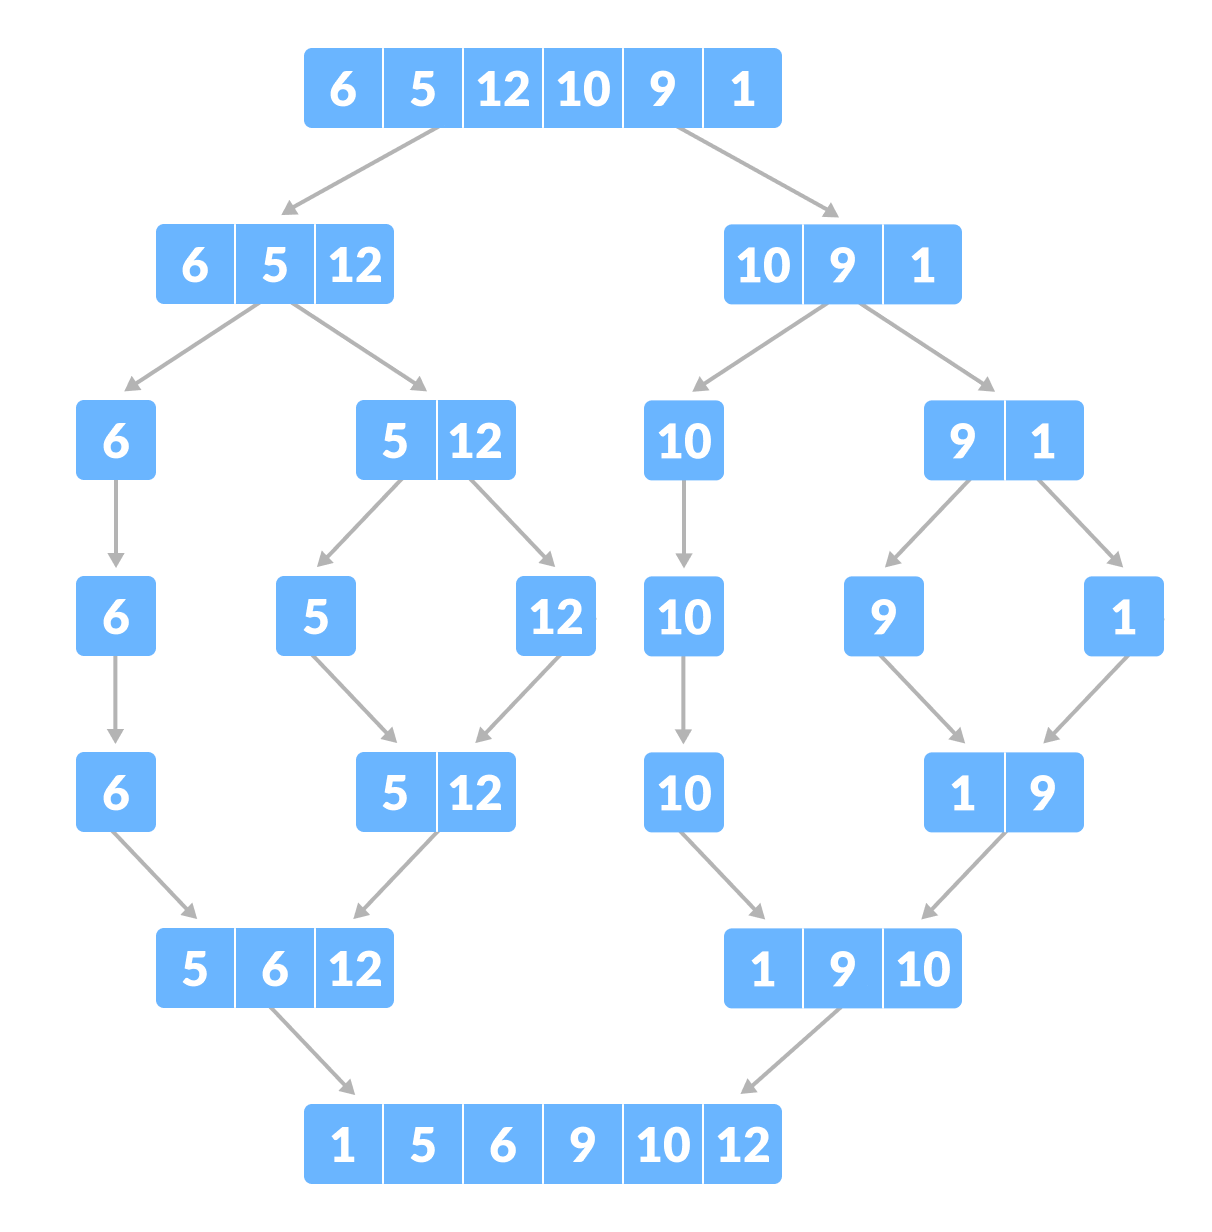
\includegraphics[scale = 0.203]{Pictures/merge-sort-example_0.png} %.203 ist max :(
        \caption{Wie MergeSort funktioniert}
        \label{fig:MergeSort1}
    \end{figure}

        \begin{figure}[h]
        \centering
        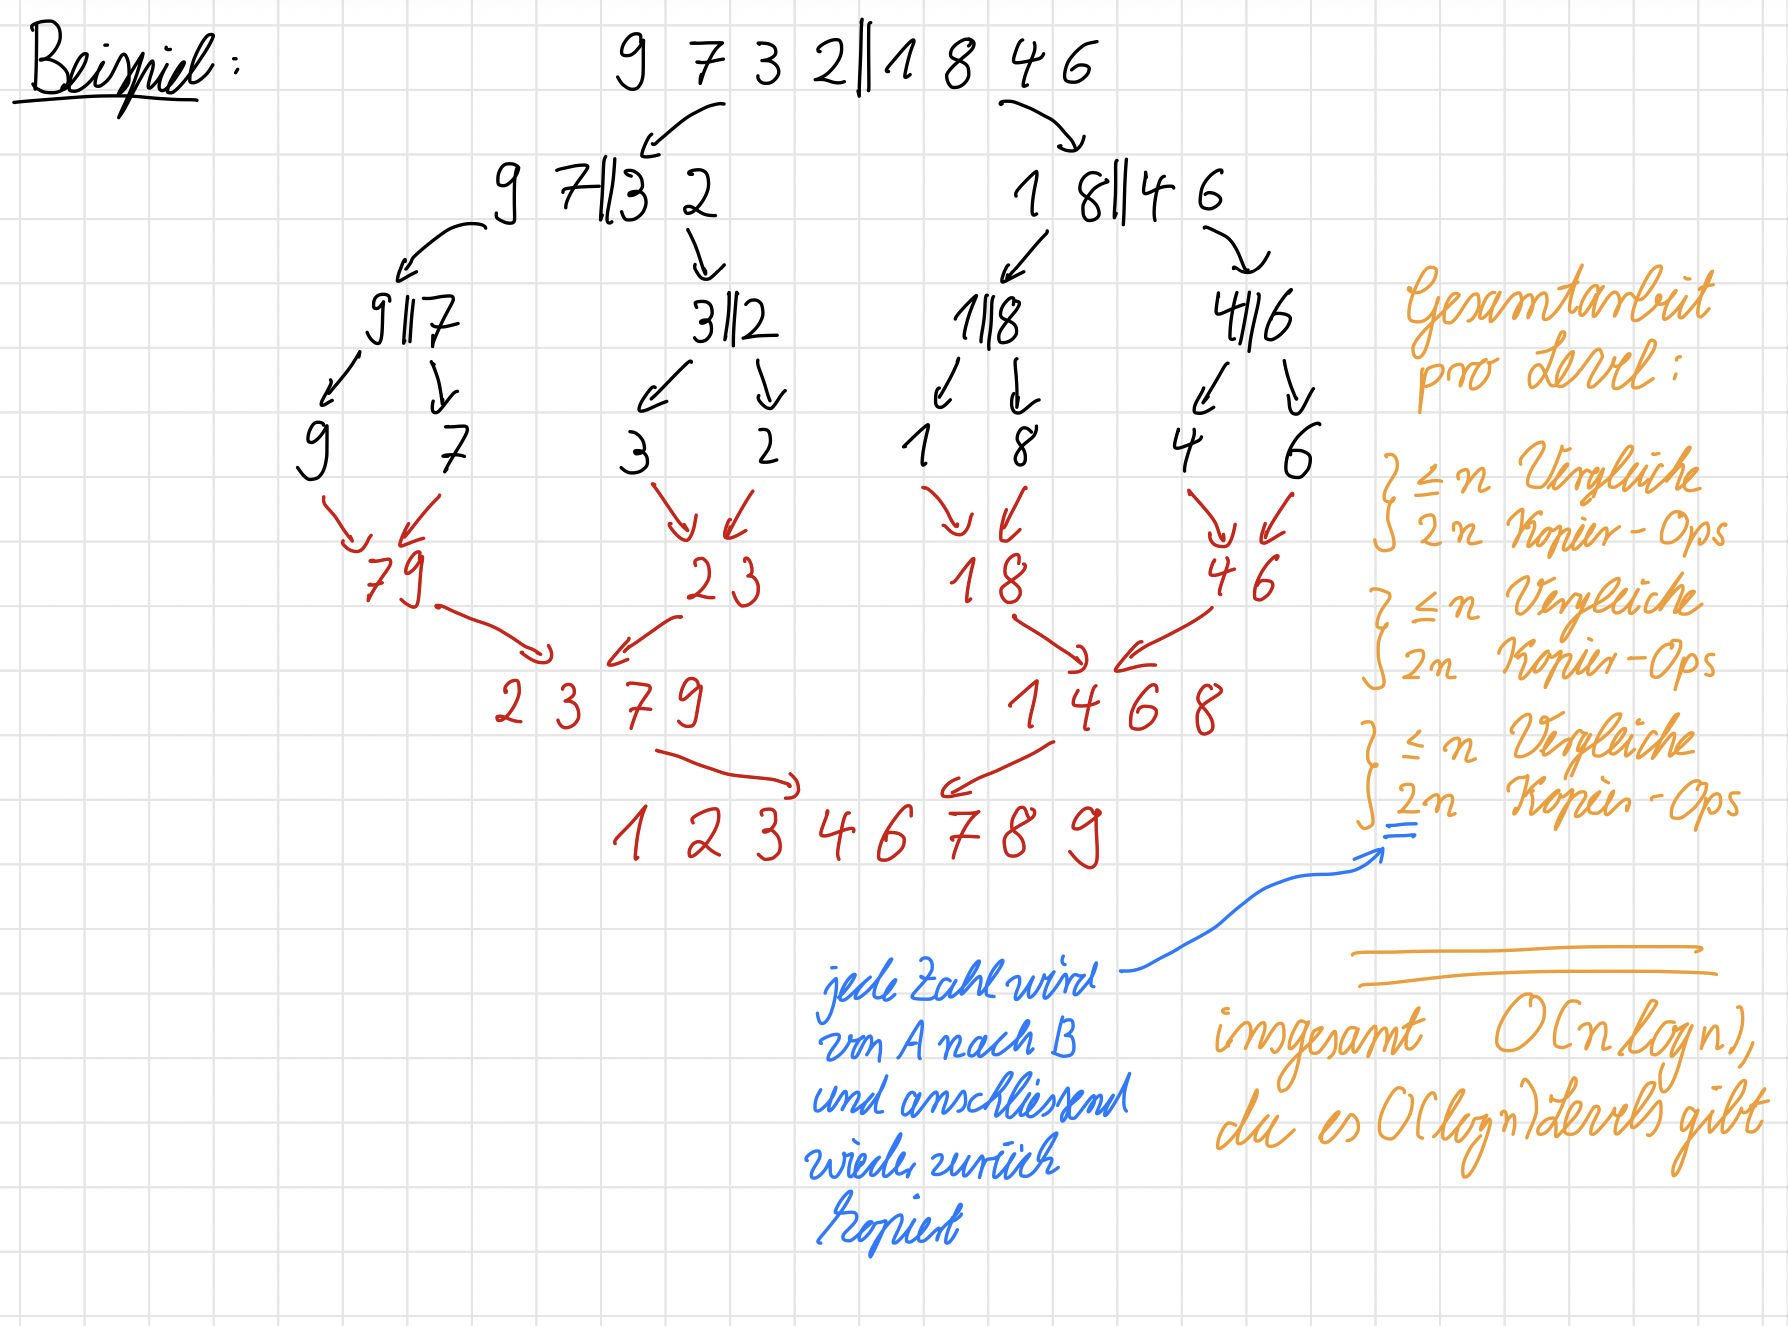
\includegraphics[width = \textwidth]{Pictures/MergeSort, Vergleiche und Schreiboperationen.png} %.203 ist max :(
        \caption{Wie MergeSort funktioniert, letzter Schritt: beide linken Elemente werden verglichen und in Array gesetzt}
        \label{fig:MergeSort2}
    \end{figure}
        
    \subsubsection{Heapsort}\label{Heapsort}
        Heapsort $\mathcal{O}(n \log n)$ - Dieser Sortieralgorithmus arbeitet, indem er alle Schlüssel in einen Min-Heap einfügt und iterativ das Minimum (die Wurzel) in konstanter Zeit extrahiert und an die Liste der sortierten Knoten anhängt. Er macht dies $n$ Mal; die Gesamtlaufzeit hängt von der Komplexität der Standard-Heap-Operationen ab.
        
        \begin{algorithm}[h]
            \caption{Heap sort}
            \label{alg:HeapSort}
            \begin{algorithmic} 
            \State $H \gets \textsc{CreateMinHeap}\left(\right)$
            \For{$i \in \left\lbrace 0, \dots, A\texttt{.length}-1 \right\rbrace$}
            \State $H\texttt{.insert}\left(A\left[i\right]\right)$
            \EndFor
            \For{$i \in \left\lbrace 0, \dots, A\texttt{.length}-1 \right\rbrace$}
            \State $v \gets H\texttt{.pop}\left(\right)$
            \State $R\texttt{.add}\left(v\right)$
            \EndFor
            \State \Return $R$
            \end{algorithmic}
        \end{algorithm}
        
    Damit Heapsort ein eher schwerer Algorithmus ist zum sich vorstellen ist die Abbildung im Anhang (\ref{fig:heapsort with array}) sehr nützlich. Diese Abbildung behandelt jedoch den \texttt{CreateMaxHeap}- Fall. Im oben beschriebenen Algorithmus wird der Fall \texttt{CreateMinHeap}  diskutiert. Der Unterschied bezüglich Min-, Max-Heap wurde in Figure \ref{fig: Min/Max-heap} beschrieben.\label{VerlinkzuHeapSortText}


    
    \subsubsection{Kosten von Sortieralgorithmen}
    Hier werden die minimalen und maximalen Kosten für einige Sortieralgorithmen auf der Grundlage ihrer Eingabegröße n angegeben, sowie die besondere Art der Eingabe, die zu dieser besonderen Komplexität führt.
    \begin{table}[H]
      \centering
      \footnotesize
      \caption{Best and worst case costs für sortier Algorithmen}
      \label{Sorting 1}
      ~\\
      \hspace{-1.6cm}
      \begin{tabular}{|l | c c | c c | c c | c c |}
        \cline{2-9}
        \multicolumn{1}{c|}{} & \multicolumn{2}{c|}{\textbf{bubblesort}} & \multicolumn{2}{c|}{\textbf{insertion sort}} & \multicolumn{2}{c|}{\textbf{selection sort}} & \multicolumn{2}{c|}{\textbf{quicksort}} \\
        \multicolumn{1}{c|}{}             & best case                & worst case                & best case                  & w.c.                  & best case                  & w.c.                  & best case               & w.c.               \\
        \hline
        \# comparisons  & $\Theta(n)$                  & $\Theta(n^2)$                  & $\Theta(n)$                    & $\Theta(n^2)$                    & $\Theta(n^2)$                    & $\Theta(n^2)$                    & $\Theta(n \log n)$                                  & $\Theta(n^2)$                 \\
        \# permutations & $0$                   & $\Theta(n^2)$                  & $0$                     & $\Theta(n^2)$                    & $0$                     & $\Theta(n)$                    & $\Theta(n)$                   & $\Theta(n \log n)$                 \\
        \hline
        corresponding order             & A                 & B                 & A                   & B & A                   & C                   & C                    & C                 \\
        \hline
      \end{tabular}
      \begin{itemize}
      \item A = already ordered
      \item B = inverse order
      \item C = special order
      \end{itemize}
    
    
    \end{table}
    
     
    \subsubsection{Lower-bound für Sortier-Algorithmen}
    Jegliche Sortieralgorithmen haben eine worst-case runtime von $\Omega(n \log n)$. Mehr dazu in \textit{Algorithmen und Wahrscheinlichkeiten, ConvexHull}
        
        

\newpage
%%Chapter 04
\section{Graphen Theorie}
Wie muss ein Rundweg durch Königsberg aussehen, auf dem ich jede Brücke über den Pregel genau einmal überquere und am Schluss zum Ausgangspunkt zurückkomme? Diese und viele andere Probleme lassen sich als Probleme in Graphen formulieren und mithilfe von Graphenalgorithmen lösen. In einem Graphen wird dabei die wesentliche Struktur des Problems, befreit von unbedeutenden Nebenaspekten, repräsentiert.
In diesem Kapitel wird auf Englisch geschrieben, da dies den Stoff vereinfacht und sowieso fast alles gleich ist. Somit: technical terms are given in both English and \textcolor{blue}{{Deutsch}}.Always make sure that your vocabulary is consistent.

\subsection{Definitions}

We usually note $G=(V,E)$ with
\begin{itemize}
\item $V=\{v_1, ..., v_n\}$, $|V|=n$ the set of nodes (\textcolor{blue}{{Knotenmenge}});
\item $E=\{e_1, ..., e_m\}$, $|E|=m$ the set of edges (\textcolor{blue}{{Kantenmenge}}).
\end{itemize}

\subsubsection{Undirected graph (\textcolor{blue}{{ungerichteter Graph}})}
Here $E\subseteq \{\{u,v\} \mid u,v\in V\}$ contains undirected edges which are denoted as $e_k=\left\lbrace v_i, v_j \right\rbrace$. Note that here $v_i$ and $v_j$ are in one \textbf{set}, which in particular implies $\left\lbrace v_i, v_j \right\rbrace = \left\lbrace v_j, v_i \right\rbrace$. Vertices $v_i$ and $v_j$ are called adjacent (\textcolor{blue}{{benachbart}} or \textcolor{blue}{{adjazent)}} iff $\left\lbrace v_i, v_j \right\rbrace \in E$ and a vertex $v_i$ and an edge $e_k$ are incident (\textcolor{blue}{{inzident}}) iff $v_i \in e_k$.


\subsubsection{Directed graph (\textcolor{blue}{{gerichteter Graph}})}
Here $E\subseteq V\times V$ are directed edges which are denoted as ordered pairs $e_k=\left(v_i, v_j\right)$. Now, $\left(v_i, v_j\right) \neq \left(v_j, v_i\right)$. Vertices $v_i$ and $v_j$ are called adjacent (\textcolor{blue}{{benachbart}} or \textcolor{blue}{{adjazent}}) iff $\left(v_i, v_j \right) \in E$ and a vertex $v_i$ and an edge $e_k$ are incident (\textcolor{blue}{{inzident}}) iff $v_i \in e_k$.

\subsubsection{Bipartite graph (\textcolor{blue}{{bipartiter Graph}})}
A graph is bipartite iff we can decompose its set of vertices into $V=U\uplus W$ two disjoint sets of nodes ($U \cap W=\emptyset$) such that
\begin{itemize}
\item Either $E\subseteq \left\lbrace \left\lbrace u,w \right\rbrace \mid u\in U, w\in W \right\rbrace$ (undirected bipartite graph); or
\item $E\subseteq (U\times W) \cup (W\times U)$ (directed bipartite graph).
\end{itemize}
We will get to see more about bipartite graphs in \textit{Algorithmen und Wahrscheinlichkeiten}.

\subsubsection{Tree (\textcolor{blue}{{Baum}}) and forest (\textcolor{blue}{{Wald}})}
A tree is a graph that is both connected (\textcolor{blue}{{zusammenhängend}}, i.e. there exists a path between all pairs of points) and acyclic (\textcolor{blue}{{azyklisch}}, i.e. contains no cycle, see below). A connected graph is a tree iff it has exactly $m=n-1$ edges.

A forest is a graph that is acyclic, but not necessarily connected. Hence, a forest can have several connected components (\textcolor{blue}{{Zusammenhangskomponenten}} \ref{ZSMkomponenten}), each of which is a tree. In short, a forest is a collection of trees. (See Figure \ref{fig:tree/forest})

\begin{figure}[h]
    \centering
    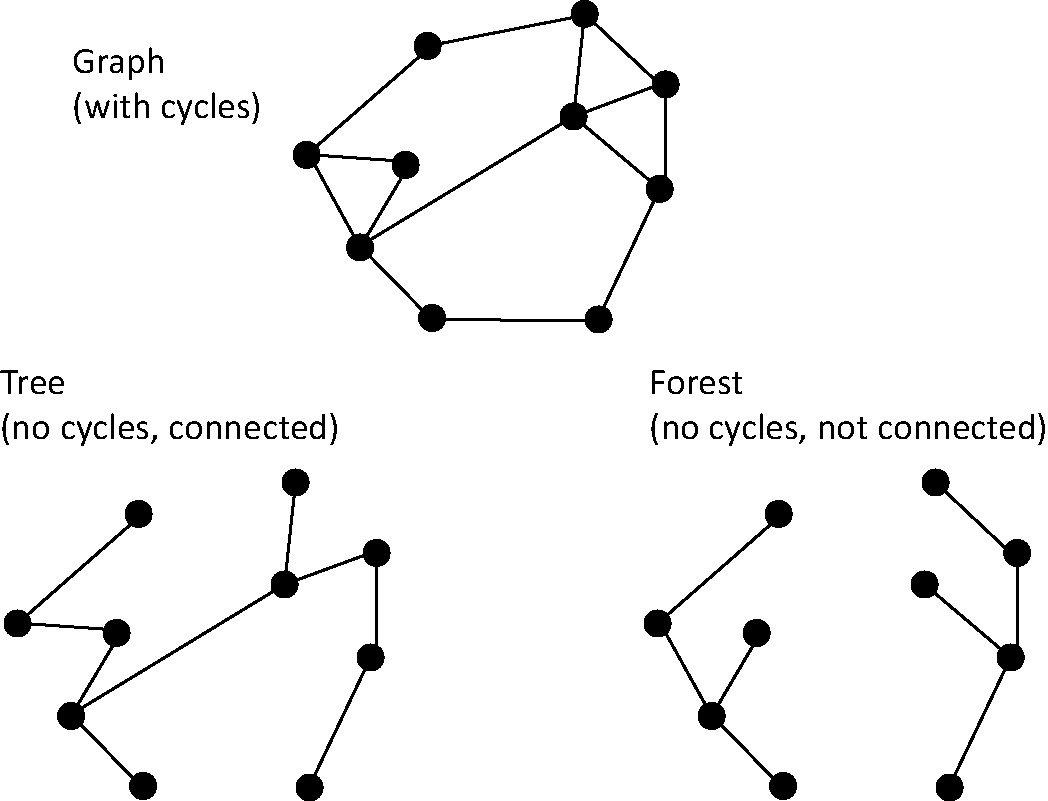
\includegraphics[scale = 0.2]{Pictures/TreeAnDForest.png}
    \caption{Tree and forest. Forest has two \textcolor{blue}{Zusammenhangskomponenten}}
    \label{fig:tree/forest}
\end{figure}

\subsubsection{Adjacency lists (\textcolor{blue}{{Adjazenzlisten}})}
The adjacency lists $L$ associate to each $v_i \in V$ the list $L\left[i\right]$ of its neighbors (\textcolor{blue}{{Nachbarn}}) in $G$, i.e.
$$L\left[i\right] = \left\lbrace v_j \in V \mid v_i\text{ and }v_j\text{ are adjacent} \right\rbrace.$$


  
\subsubsection{Adjacency matrix (\textcolor{blue}{{Adjazenzmatrix}})}
Let $n=|V|$. The adjacency matrix $A$ is defined as:
$$A\in \{0,1\}^{n\times n}$$
where
$$a_{i,j}=\begin{cases} 1 & \text{if }v_i\text{ and }v_j\text{ are adjacent} \\ 0 & \text{otherwise} \end{cases}$$
In particular, this definition implies that, for undirected graphs, $A$ is symmetric.
The particular case $a_{i,i}=1$ means that there is a loop on node $v_i$. This is possible on both directed and undirected graphs, and depends on the definition of graph given and the allowed cases.

\subsubsection{What can or cannot we have in a graph?}

\emph{In general}, `standard' graphs (=what will be called graphs in the exam) \textbf{do not}
\begin{itemize}
\item Contain several parallel edges between the same pair of nodes---allowing this to happen would make our graph a \textbf{multigraph} (\textcolor{blue}{{Multigraph}}); (See Figure \ref{fig:Multigraph})
\item Contain hyperedges, i.e. edges with more than two endpoints---allowing this to happen would make our graph a \textbf{hypergraph} (\textcolor{blue}{{Hypergraph}}) (See Figure \ref{fig:Hypergraph}).
\end{itemize}
`Standard' graphs may or may not contain (self-)loops (\textcolor{blue}{{Schleifen}}). The A\&D Skript considers that `standard' graphs may contain loops.

\begin{figure}
    \begin{subfigure}{0.3\textwidth}
        \centering
        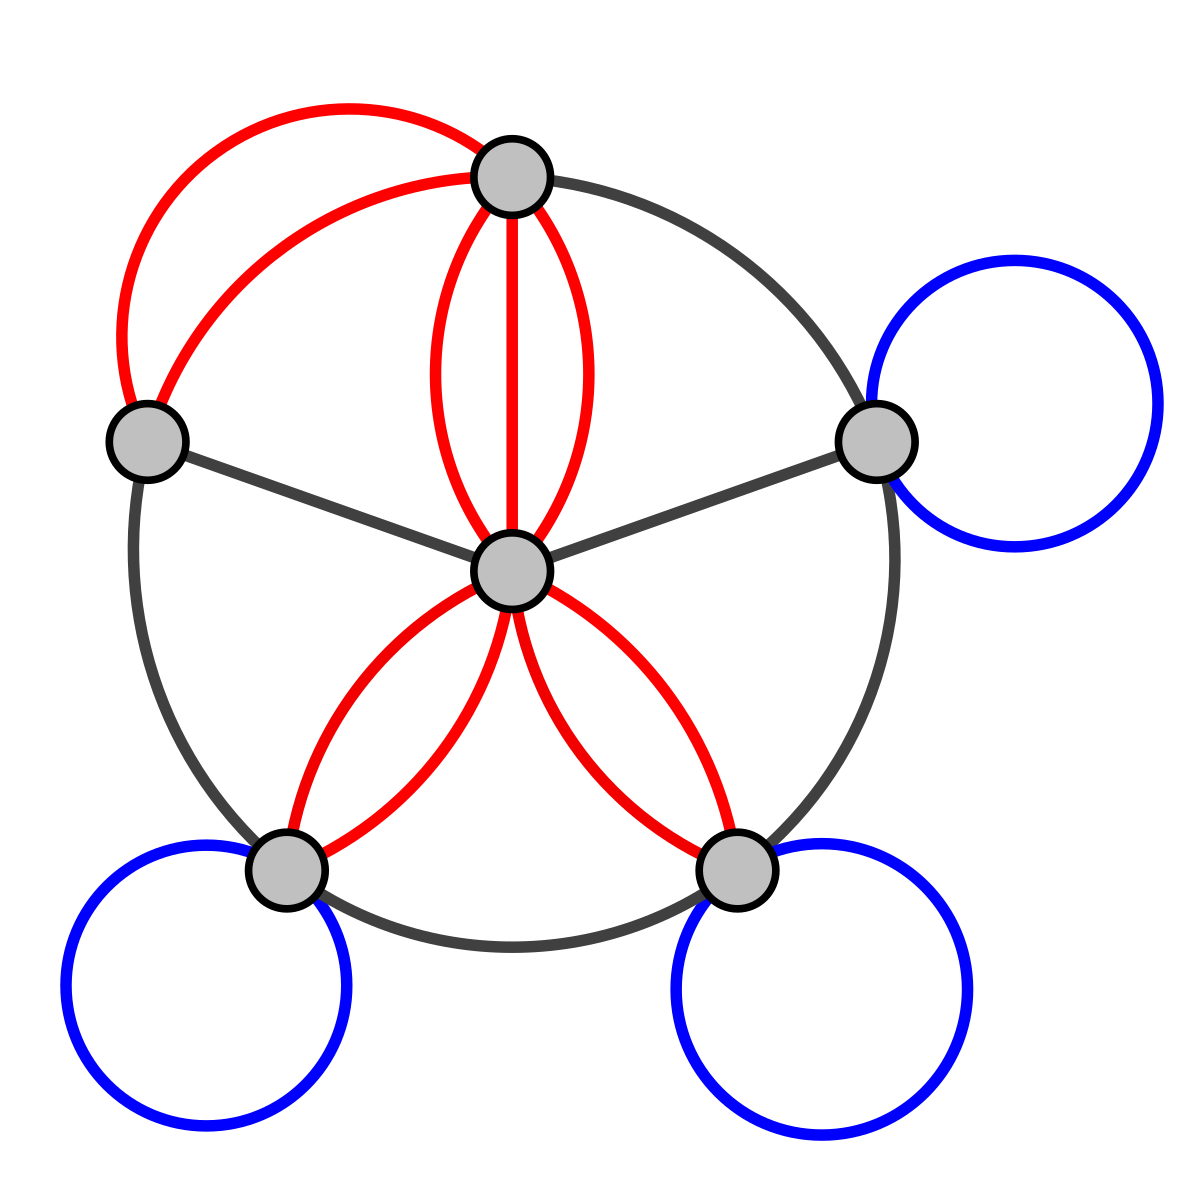
\includegraphics[width=\textwidth]{Pictures/Multi-pseudograph.svg.png}
        \caption{How a multigraph looks like}
        \label{fig:Multigraph}
    \end{subfigure}
    \hfill
    \begin{subfigure}{0.3\textwidth}
        \centering
        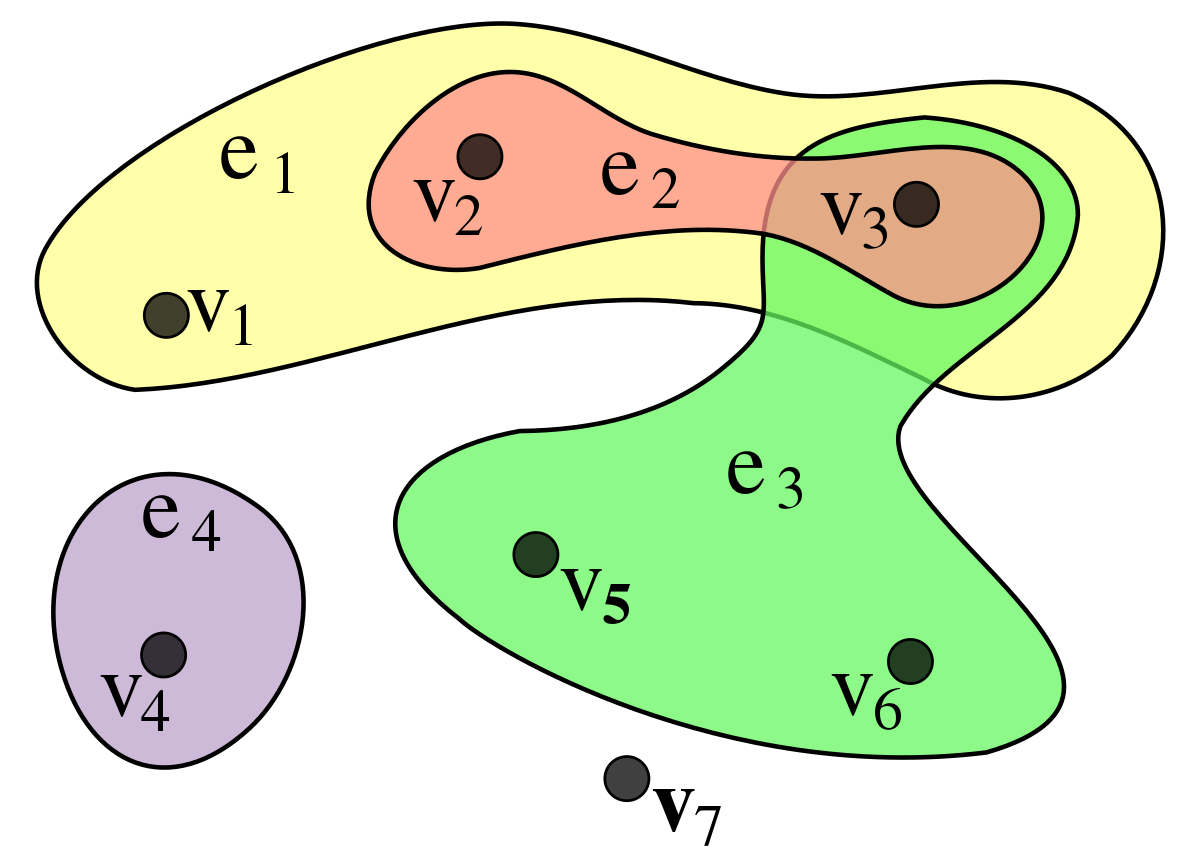
\includegraphics[width=\textwidth]{Pictures/1200px-Hypergraph-wikipedia.svg.png}
         \caption{How a hypergraph looks like}
        \label{fig:Hypergraph}
    \end{subfigure}
\caption{Multi- und Hypergraph}
\label{fig:MultiHyperGraph}
\end{figure}
    
\subsubsection{Sequences}

Consider the sequence of vertices
$$\langle v_1, v_2, ..., v_k\rangle \in V^k.$$

This sequence is
\begin{itemize}
\item A \textbf{walk} (\textcolor{blue}{{Weg}}) iff there are edges between $v_i$ and $v_{i+1}$ for all $i\in\{1, \dots, k-1\}$; in this case, the length of the walk is $k-1$;
\item A \textbf{path} (\textcolor{blue}{{Pfad}}) iff it is a walk whose vertices are all distinct;
\item A \textbf{tour} (\textcolor{blue}{{Reise}}) iff it is a walk whose edges are all distinct;
\item A \textbf{circuit} (\textcolor{blue}{{Zyklus}}) iff it is a walk with $v_1 = v_k$ (starts and ends at the same vertex);
\item A \textbf{cycle} (\textcolor{blue}{{Kreis}}) iff it is a circuit for which no vertex, except the first/last one, is visited more than once;
\item A \textbf{loop} (\textcolor{blue}{{Schleife}}) iff it is a cycle $\langle v_i, v_i\rangle$ of length 1.
\end{itemize}

When the considered objects cover all vertices or all objects, this gives rise to the following definitions:
\begin{itemize}
\item A \textbf{Eulerian walk} (\textcolor{blue}{{Eulerweg}}) is a walk that visits all edges exactly once, i.e. a walk of length $m = |E|$.

\item A \textbf{Eulerian circuit} (\textcolor{blue}{{Eulerkreis}} \footnote{Note that this terminology is not consistent with the above definition of \textcolor{blue}{Kreis}; The German translation of the following definition is \textcolor{blue}{"Ein Eulerkreis ist ein \textbf{Zyklus}, der alle Kanten des Graphens genau einmal durchläuft, d.h. ein Zyklus der Länge $m$.}}) is a circuit that visits all edges exactly once, i.e. a walk of length $m = |E|$.
\item A \textbf{Hamiltonian path} (\textcolor{blue}{{Hamiltonpfad}}) is a path that visits all vertices exactly one, i.e. a path of length $n-1$.
\item A \textbf{Hamiltonian circuit} (\textcolor{blue}{{Hamiltonkreis}} \footnote{No consistency problem here; the German definition is \textcolor{blue}{"Ein Hamiltonkreis ist ein Kreis, der alle Knoten durchläuft, d.h. ein Kreis der Länge $n$.}}) is a cycle that visits all vertices, i.e. a cycle of length $n$.
\end{itemize}


\subsubsection{Degree of a vertex}
The degree (or valency) of a vertex $v$ of a graph is the number of edges incident to this vertex, with loops counted twice. It is denoted by $\deg(v)$.

In directed graphs, we distinguish between the \textit{in-degree} $\deg^-(v)$ and the \textit{out-degree} $\deg^+(v)$.

\subsubsection{Neighborhood}
The neighborhood of some vertex $v$ (set of vertices adjacent to $v$) is denoted by $N(v)$. We have $\deg\left(v\right)=\left\lvert N\left(v\right) \right\rvert$.

In directed graphs, we again distinguish between $N^-\left(v\right)$ and $N^+\left(v\right)$. We have $\deg^-(v)=|N^-(v)|$ and $\deg^+(v)=|N^+(v)|$.

\subsubsection{Degree-sum formula (handshaking lemma)}
$$\sum_{v\in V} \deg(v)=2|E|=2m$$

\subsubsection{Runtimes of Adjacency matrix and Adjacency List}
The big difference between the adjacency matrix and the adjacency list is in the operations that are carried out. The following table shows how long it takes to perform each interaction or operation on the corresponding list or matrix:

\begin{table}[h]
    \centering
    \begin{tabular}{p{5cm}|p{1.8cm}|p{4.5cm}|p{4.5cm}}
        \toprule
        \textbf{Query} & \textbf{Adjacency Matrix} & \textbf{Adjacency List} & \textbf{Improved Adjacency List} \\
        \midrule
        (a) Find $deg(v)$ & $\Theta(n)$ & $\Theta(1 + \text{deg}(v))$ & $\Theta(1)$ \\
        (b) Find a neighbor of $v$ & $\Theta(n)$ & $\Theta(1)$ & $\Theta(1)$ \\
        (c) Decide if $u$ and $v$ are adjacent & $\Theta(1)$ & $\Theta(1 + \min\{\text{deg}(v), \text{deg}(u)\})$ & $\Theta(1 + \min\{\text{deg}(v), \text{deg}(u)\})$ \\
        (d) Delete edge $\{u, v\}$ & $\Theta(1)$ & $\Theta(\text{deg}(v) + \text{deg}(u))$ & $\Theta(\min\{\text{deg}(v), \text{deg}(u)\})$ \\
        (e) Find neighbor $v$ of $u$ and delete $\{u, v\}$ & $\Theta(n)$ & $\Theta(1 + \max \{\text{deg}(w)\})$ & $\Theta(1)$ \\
        (f) Insert edge $\{u, v\}$ if not exists & $\Theta(1)$ & $\Theta(1 + \min\{\text{deg}(v), \text{deg}(u)\})$ & $\Theta(1 + \min\{\text{deg}(v), \text{deg}(u)\})$ \\
        (g) Delete vertex $v$ and incident edges & $\Theta(n^2)$ & $\Theta(n + m)$ & $\Theta(n)$ \\
        (h) Find all neighbour of $v$  & $\Theta(n)$ & $\Theta(\text{deg}_{out}(v))$ &  \\
        (i) Find $v \in V$ without neighours & $\Theta(n^2)$ & $\mathcal{O}(n)$ &  \\
        (j) Is $(u,v) \in V$  & $\Theta(1)$ & $\Theta(1)$ & $\Theta(1)$ \\
        (k) Insert edge & $\Theta(1)$ & $\Theta(\text{deg}_{out}(v))$ & \\

        \bottomrule


        
    \end{tabular}
    \caption{Query Runtimes in $\Theta$-Notation for Different Representations}
    \label{tab:runtimes}
\end{table}

\newpage
    
\subsection{Overall Data Structures}
\subsubsection*{Abstrakte Datentypen (ADT)}
ADT beschreiben die \textbf{Ziele:} \underline{Was} wollen wir mit den Daten tun? \\
ADT: \textsc{Objekte + Operationen}, Hier: \textsc{Objekte} = Schlüssel $\in \mathbb{N}$\\


\subsubsection*{Datenstruktur = Implementierung eines ADT}
Datenstrukturen beschreiben: \underline{Wie} realisieren wir einen ADT im Speicher?

\begin{itemize}
    \item ADT-Liste
    \item Array
    \item Linked-List
    \item Doubly-Linked-List
\end{itemize}
Jede dieser Datenstrukuten verfügt über die in Section (\ref{common operations}) besprochenen Operationen:
\begin{itemize}
    \item \texttt{insert}$(K, L)$, fügt ein Objekt mit Schlüssel $K$ am Ende der Liste an
    \item \texttt{get}$(i L)$,  gibt $i$-ten Schlüssel aus
    \item \texttt{delete}$(o, L)$, lösche Objekt $o$ aus Liste
    \item \texttt{insertAfter}$(o, K, L)$, füge Objekt mit Schlüssel $K$ hinter $o$ ein
\end{itemize}

    \begin{table}[H]
      \centering
      \footnotesize
      \caption{Kosten für Operationen auf versch. Datenstrukturen; mit $^*$ markierte bedeuten, dass wir im Speicherort das Objekt $o$ kennen}
      \label{tab:Costs on Datastructures}
      ~\\ 
      \hspace{-1.6cm}
      \begin{tabular}{|l | c | c | c | c |}
      \hline
        \textbf{} & 
        \textbf{\texttt{insert}} & 
        \textbf{\texttt{get}} &
        \textbf{\texttt{delete}} &
        \textbf{\texttt{insertAfter}} \\
        \hline
        Array & 
        $\mathcal{O}(1)$ & 
        $\mathcal{O}(1)$ &
        $\mathcal{O}(n)$ &
        $\mathcal{O}(n)$ \\
        Linked-List & 
        $\mathcal{O}(n)$ & 
        $\mathcal{O}(n)$ &
        $\mathcal{O}(n)$ &
        $\mathcal{O}(1)^*$ \\
        Doubly-LinkedList & 
        $\mathcal{O}(1)$ & 
        $\mathcal{O}(n)$ &
        $\mathcal{O}(1)^*$ &
        $\mathcal{O}(1)^*$ \\
        \hline
      \end{tabular}
    \end{table}

\subsubsection{Stacks and Queues}
Stacks and queues are two elementary ADS that can be implemented with (doubly-)linked lists.

\subsubsection*{Stack}
\texttt{LIFO} - Last in, First out data structure: Inserted elements are retrieved by inverse order of insertion
    \begin{itemize}
        \item \texttt{PUSH}$(x)$ : push an object $x$ on top of the stack
        \item \texttt{POP} : removes \textbf{last} object added to stack. Throws error if stack is empty.
    \end{itemize}
    
\subsubsection*{Queue}
\texttt{FIFO} - First in, First out data structure: Inserted elements are retrieved by order of insertion
    \begin{itemize}
        \item \texttt{ENQUEUE}$(x)$ : adds an object $x$ at the end of the queue.
        \item \texttt{DEQUEUE} : removes \textbf{first} object added to the queue. Throws error if stack is empty.
    \end{itemize}

\subsubsection*{Additional methods about Stack and Queue}

Methods \textsc{enqueue} and \texttt{dequeue} might be also called \texttt{push} and \texttt{pop}. In addition, stacks and queues might share several methods which allow for testing emptyness (\texttt{isEmpty}), returning length (\texttt{length}), returning the head element (top or end) without deleting it (\texttt{head})  or deleting all elements (\texttt{clear}).
An essential observation is that all operations above (except \texttt{clear}) have constant-time runtime complexity.

\begin{figure}[h]
    \centering
    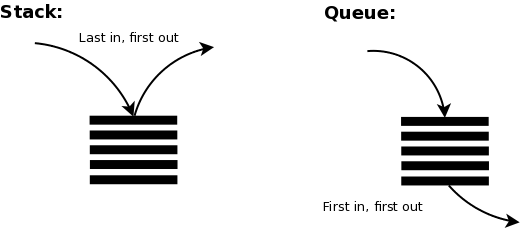
\includegraphics[scale = 0.5]{Pictures/Stack and Queue.png}
    \caption{Stack and Queue visualized}
    \label{fig:Queue and Stack}
\end{figure}

    
\subsection{ Depth-first Search (\textcolor{blue}{Tiefensuche})}
Depth-first search $\mathcal{O}(n+m)$ is an algorithm for traversing or searching tree or graph data structures. The algorithm starts at the root node (can be selected arbitrary in a graph) and explores as far as possible along each branch before backtracking. The following Figure \ref{fig:DFS-Veranschaulichung} shows us how the DFS algorithm traverses through the graph. The Algorithm uses $\mathcal{O}(n+m)$ auxiliary space, since an extra visited array of size $V$ is needed and a stack size for iterative call to DFS function.

\begin{figure}[h]
    \begin{subfigure}{0.4\textwidth}
        \centering
        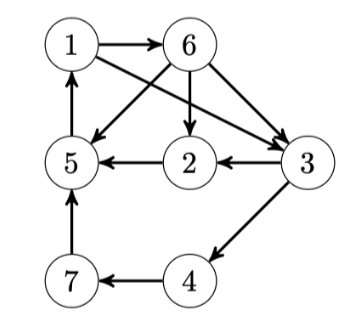
\includegraphics[scale = 0.4, width=\textwidth]{Pictures/DFS-StartGraph.png}
        \caption{Originial Graph that needs to be traversed with starting point 1}
        \label{fig:DFS-Start}
    \end{subfigure}
    \hfill
    \begin{subfigure}{0.4\textwidth}
        \centering
        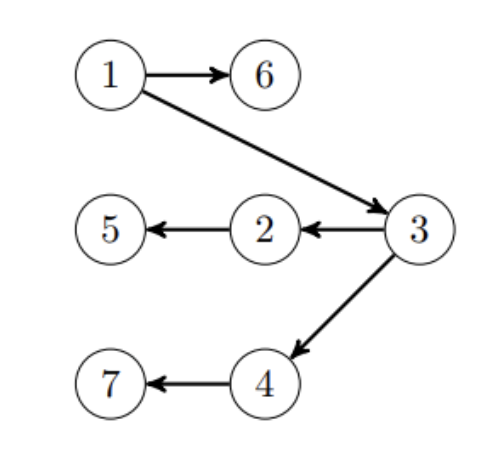
\includegraphics[scale= 0.4,  width=\textwidth]{Pictures/DFS-EndGraph.png}
         \caption{How the DFS-Algorithm traversed through graph}
        \label{fig:DFS-End}
    \end{subfigure}
\caption{Traversing through graph with DFS}
\label{fig:DFS-Veranschaulichung}
\end{figure}

The DFS-Algorithm can be implemented by two methods: Recursive or iterative.
\begin{algorithm}[H]
  \caption{Depth-first search, recursive style}
  \begin{algorithmic}
    \Function{DFS}{$v$, $G$, $D = \emptyset$}
    \State /*do something with $v$*/
    \For{$w$ s.t. $v$ and $w$ are adjacent in $G$}
    \If{$w \not\in D$}
    \State $D \gets D \cup \left\lbrace w \right\rbrace$
    \State $\textsc{DFS}\left(w, G, D \right)$
    \EndIf
    \EndFor
    \EndFunction
    \label{alg:DFS-Recursive}
    \State $\textsc{DFS}\left(s, G\right)$
  \end{algorithmic}
\end{algorithm}

\begin{algorithm}[H]
  \caption{Depth-first search, imperative style}
  \begin{algorithmic}
    \State $S \gets \texttt{new}~\texttt{stack}\left(\right)$
    \State $S\textsc{.push}\left(r\right)$
    \State $D \gets \left\lbrace r \right\rbrace$
    \While{$\neg S\textsc{.isEmpty}\left(\right)$}
    \State $v \gets S\textsc{.pop}\left(\right)$
    \State /*do something with $v$*/
    \For{$w$ s.t. $v$ and $w$ are adjacent in $G$}
    \If{$w \not\in D$}
    \State $S\textsc{.push}\left(w\right)$
    \State $D \gets D \cup \left\lbrace w \right\rbrace$
    \EndIf
    \EndFor
    \EndWhile
        \label{alg:DFS-Iterative}
  \end{algorithmic}
\end{algorithm}

\subsubsection{Zusammenhangskompontenten}\label{ZSMkomponenten}
    As seen in Figure \ref{fig:tree/forest} we have so called "Zusammenhangskomponenten". These ZHK's can be sectioned into three groups: \textbf{ back-edges, forward-edges, cross-edges}.

    To get a better understanding of how those three edges are being constructed we first have to introduce \textcolor{red}{pre/post}-numbers. We best look at them in an example to see what they are doing and how we can picture them. 
\begin{figure}[h]
    \begin{subfigure}{1\textwidth}
        \centering
        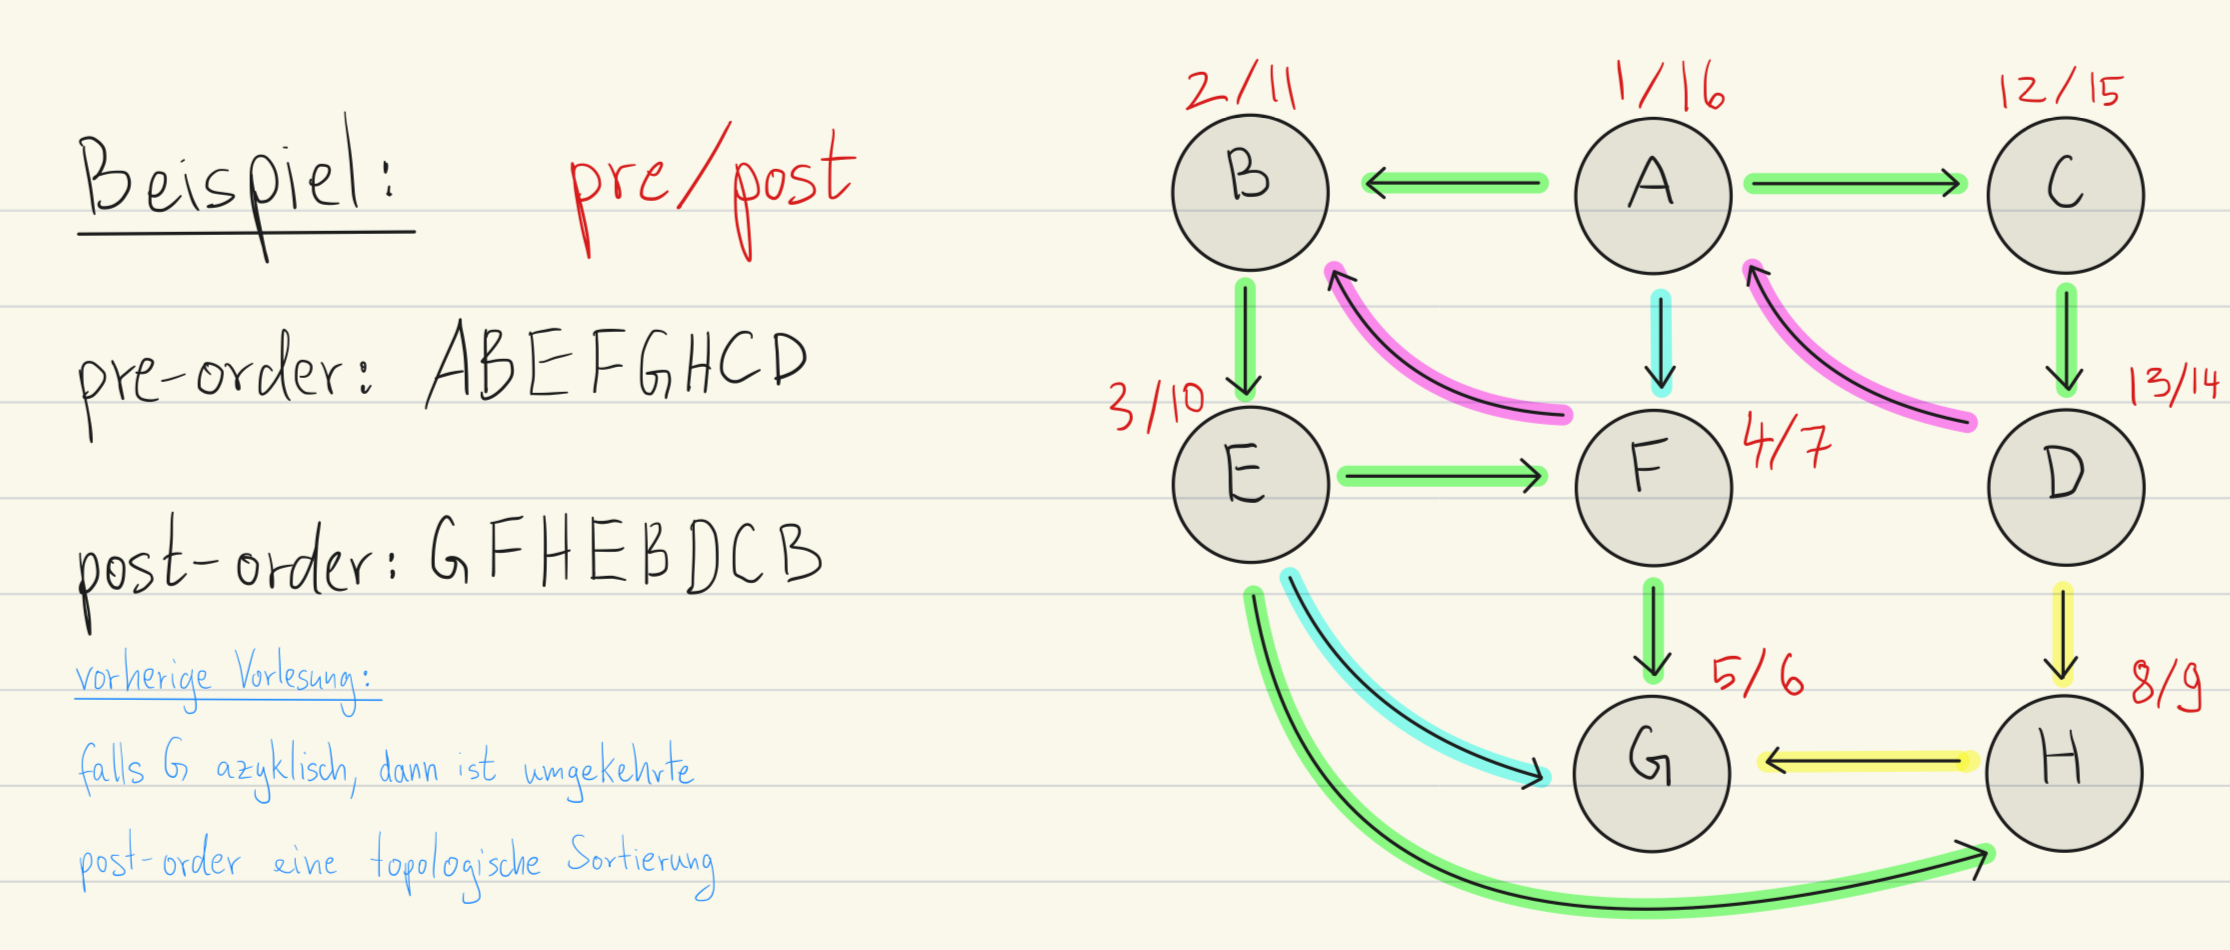
\includegraphics[scale = 0.7, width=\textwidth]{Pictures/PrePost.png}
        \caption{\textcolor{red}{Pre-/Post} numbers}
        \label{fig:Pre/PostNumbers}
        \end{subfigure}
    \hfill \\
    \begin{subfigure}{1\textwidth}
        \centering
        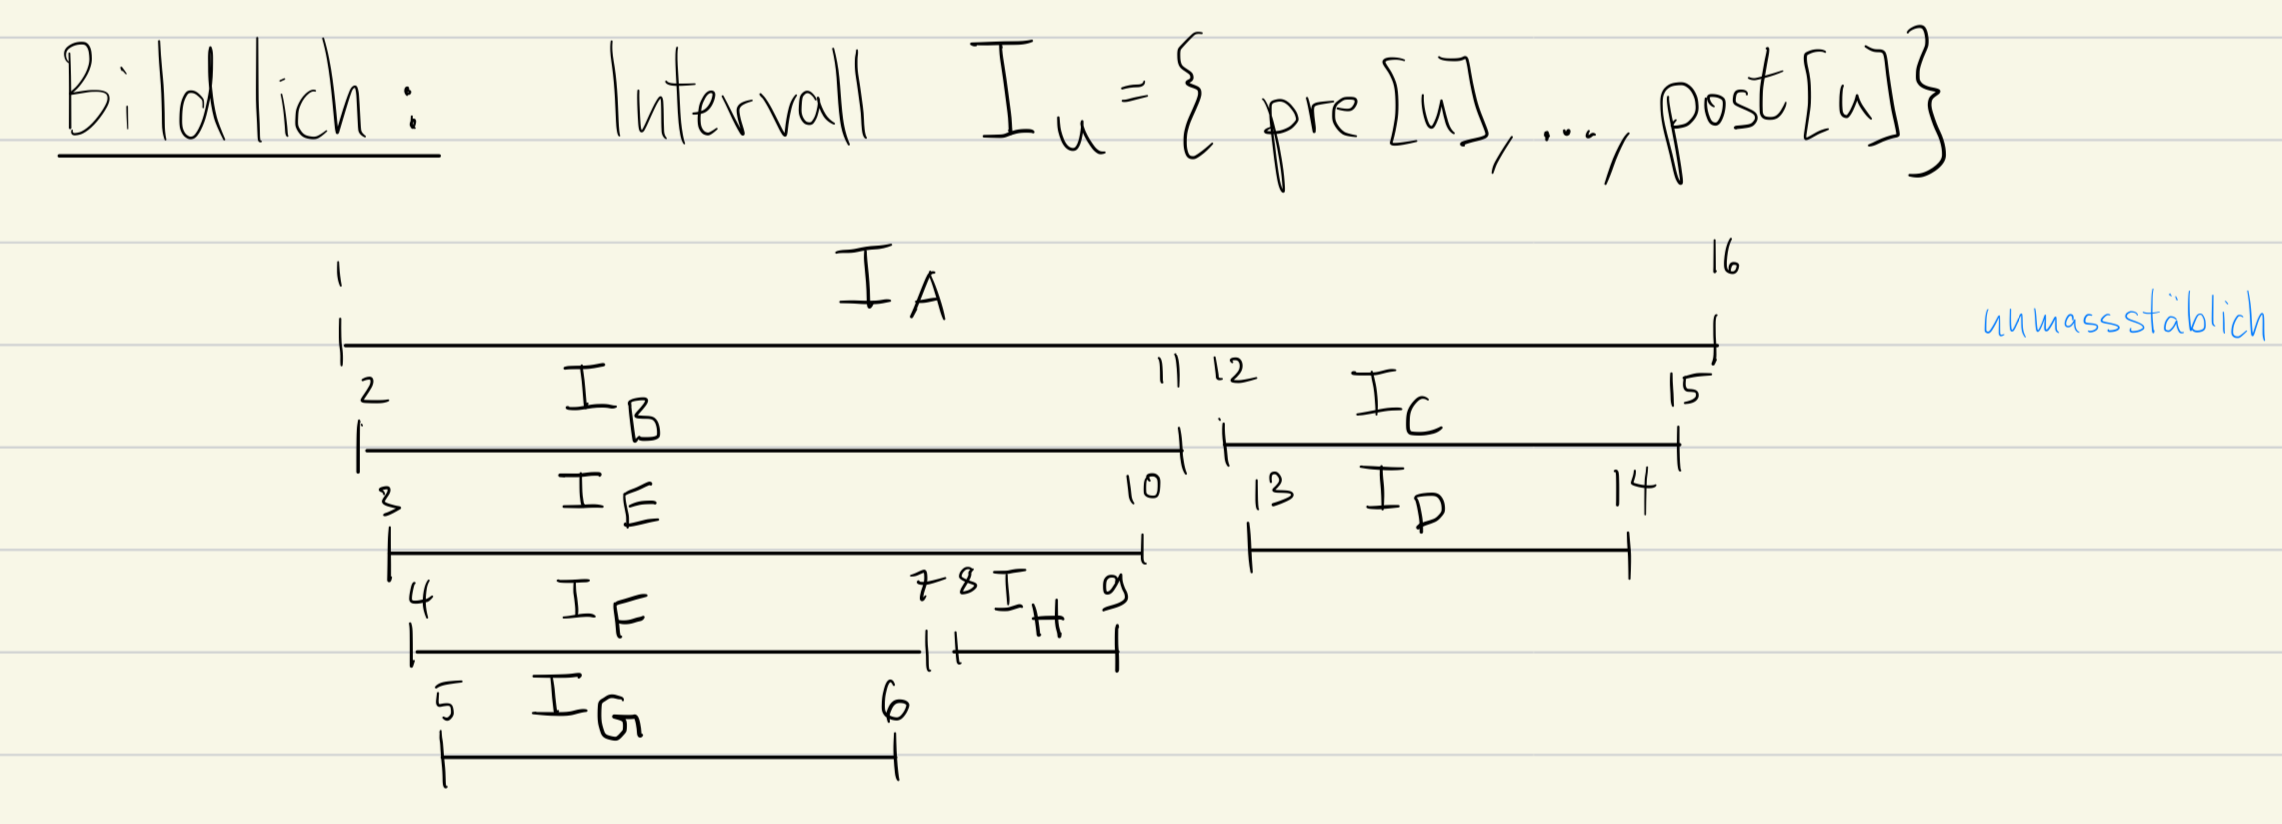
\includegraphics[scale = 0.7, width=\textwidth]{Pictures/PrePostIntrval.png}
         \caption{How \textcolor{red}{Pre-/Post} numbers can be displayed (not scaled)}
        \label{fig:DFS-End}
    \end{subfigure}
\caption{\textcolor{red}{Pre-/Post} numbers visualized}
\label{fig:BFS-Veranschaulichung}
\end{figure}

\begin{figure}[h]
    \centering
    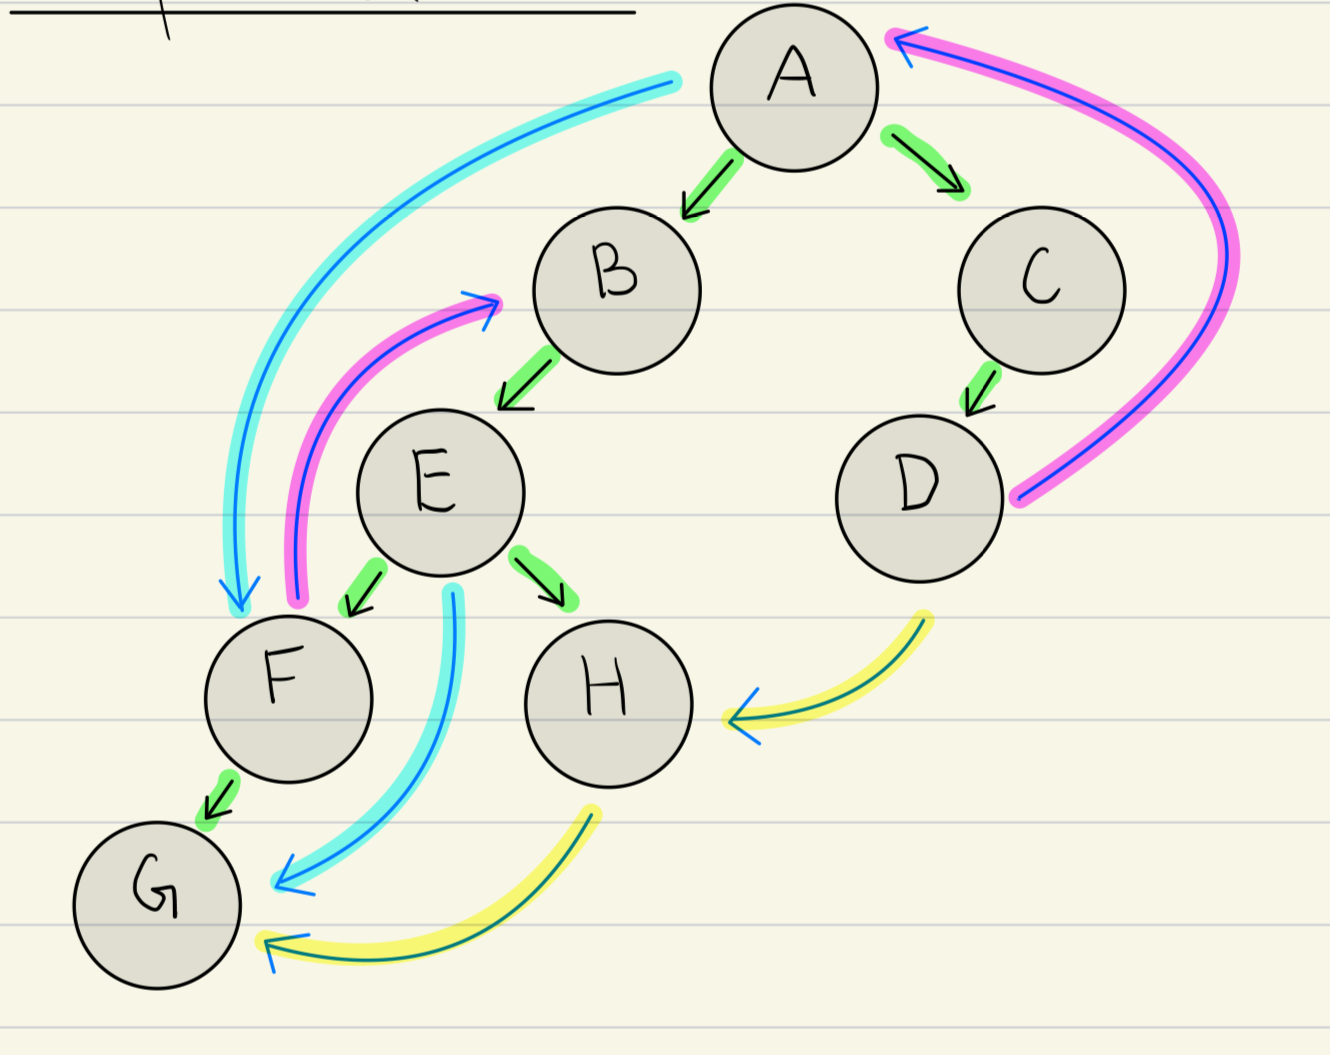
\includegraphics[scale = 0.35]{Pictures/PrePostIntrvalOrdered.png}
    \caption{Rearranged Graph}
    \label{fig:BackCrossForwardEdges}
\end{figure}
We see that if we rearrange our graph we get can clearly see the \textcolor{purple}{back-}, \textcolor{cyan}{forward-} and \textcolor{yellow}{cross-edges}. Where if we analyize their intervals it looks like: 

\begin{figure}[h]
    \centering
    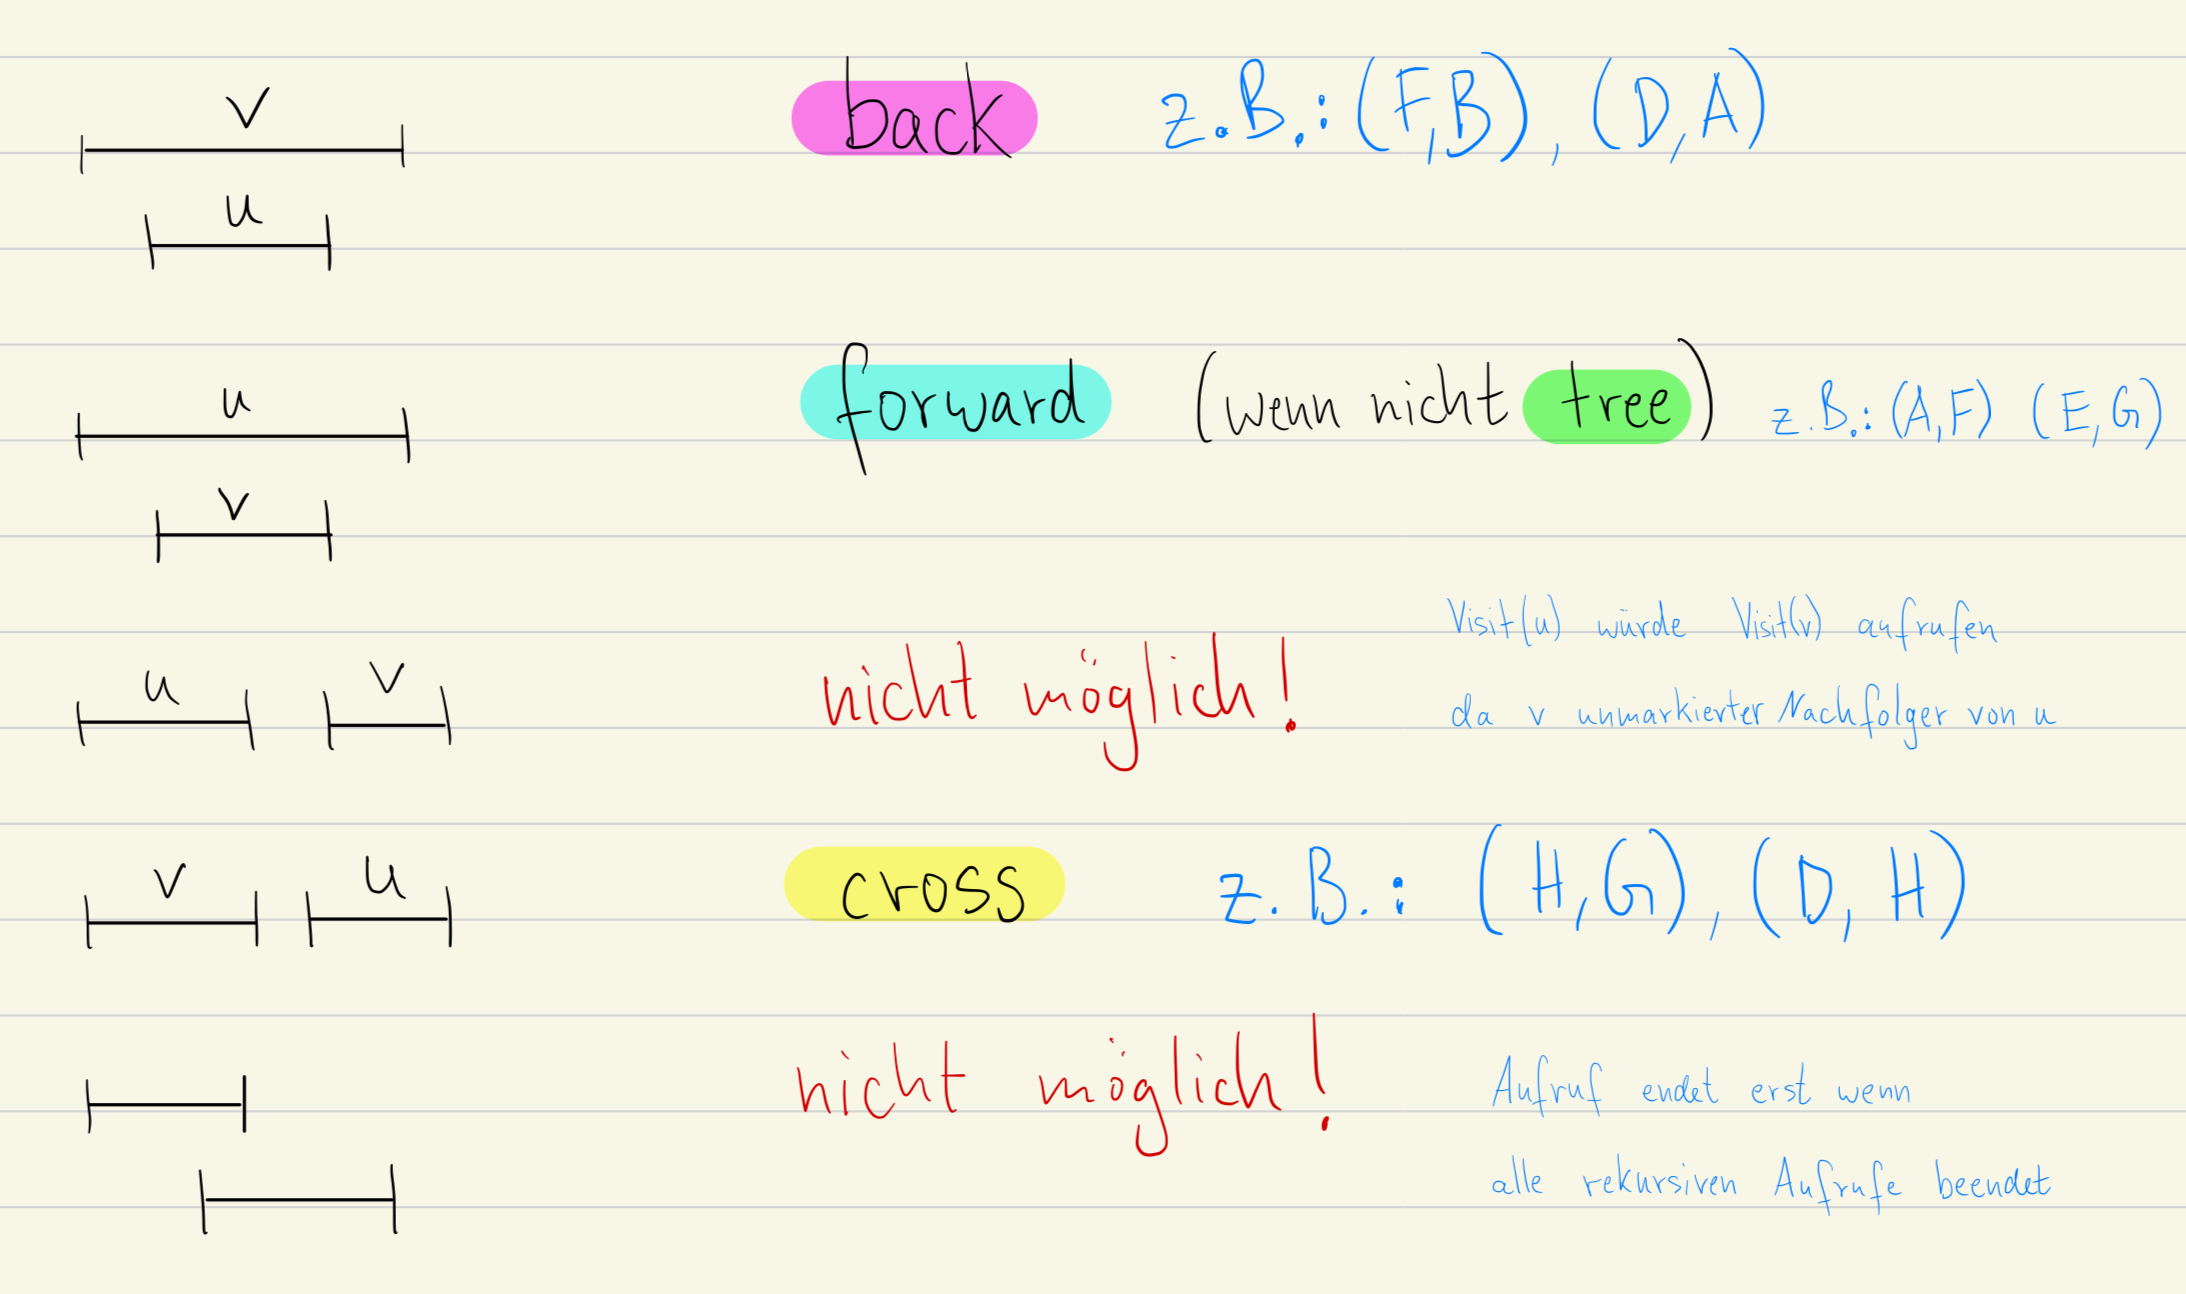
\includegraphics[scale = 0.3]{Pictures/PrePostIntrvalOrderedIn.png}
    \caption{Intervals of \textcolor{purple}{back-}, \textcolor{cyan}{forward-} and \textcolor{yellow}{cross-edges} }
    \label{fig:IntervalsofCrossEdges}
\end{figure}

We can now make following Observations: 
\begin{enumerate}
    \item $\exists$ \textcolor{purple}{back}-edge $\implies \exists$ gerichteter Zyklus
    \item $\forall$ nicht-\textcolor{purple}{back}-edge $(u,v) \in E$ : $post(u) \geq post(v)$ \\
    $\implies \nexists$ gerichteter Zyklus $\implies \nexists$  \textcolor{purple}{back}-edge $\implies$ umgekehrte $post$-order ist \textbf{topologische Sortierung} (Vgl. Figure \ref{fig:topOrdering})
\end{enumerate}
\begin{figure}[h]
    \centering
    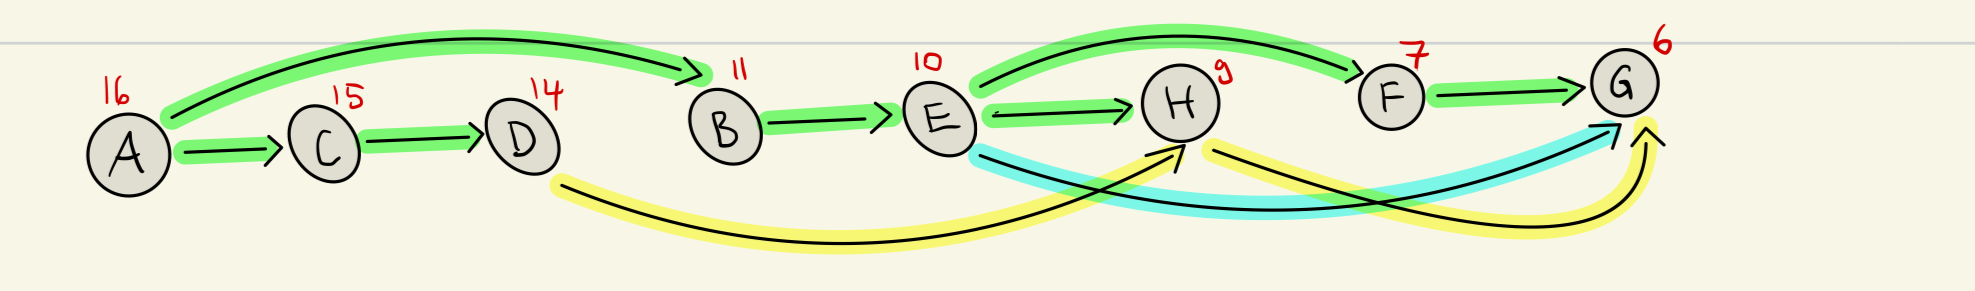
\includegraphics[scale = 0.35]{Pictures/Topologicalordering.png}
    \caption{Topological-Ordering}
    \label{fig:topOrdering}
\end{figure}

\newpage 
\subsection{Breadth-First Search (\textcolor{blue}{Breitensuche})}
    Breadth-first search $\mathcal{O}(n+m)$ is an algorithm used to search a graph data structure for a node that meets a set of criteria. It starts at the root of the graph and visits all nodes at the current depth level before moving on to the nodes at the next depth level.

    \begin{figure}[h]
    \begin{subfigure}{0.4\textwidth}
        \centering
        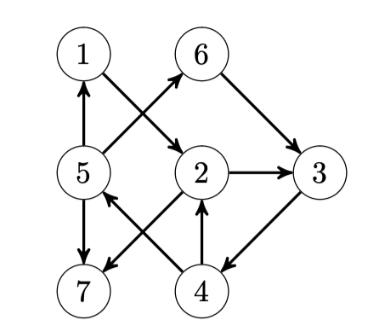
\includegraphics[scale = 0.4, width=\textwidth]{Pictures/BFS-StartGraph.png}
        \caption{Originial Graph that needs to be traversed with starting point 2}
        \label{fig:BFS-Start}
    \end{subfigure}
    \hfill
    \begin{subfigure}{0.35\textwidth}
        \centering
        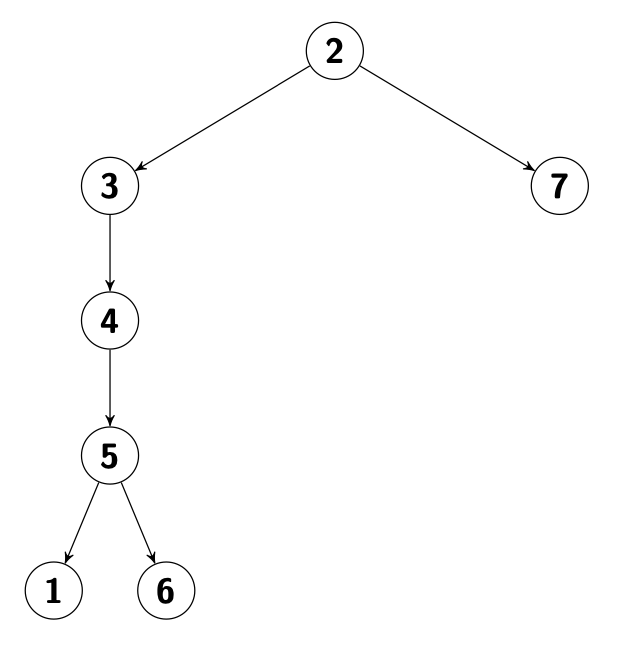
\includegraphics[scale= 0.4,  width=\textwidth]{Pictures/BFS-EndGraph.png}
         \caption{How the BFS-Algorithm traversed through graph}
        \label{fig:DFS-End}
    \end{subfigure}
\caption{Traversing through graph with BFS}
\label{fig:BFS-Veranschaulichung}
\end{figure}

In BFS, nodes are explored from a root $r$ by order of increasing distance to the root.
\begin{algorithm}[H]
  \caption{Breadth-first search}
  \begin{algorithmic}
    \State $Q \gets \texttt{new}~\texttt{queue}\left(\right)$
    \State $Q\textsc{.push}\left(r\right)$
    \State $D \gets \left\lbrace r \right\rbrace$ \Comment{Stores nodes that are done (in $Q$ or already processed)}
    \While{$\neg Q\textsc{.isEmpty}\left(\right)$}
    \State $v \gets Q\textsc{.pop}\left(\right)$
    \State /*do something with $v$*/
    \For{$w$ s.t. $v$ and $w$ are adjacent in $G$}
    \If{$w \not\in D$}
    \State $Q\textsc{.push}\left(w\right)$
    \State $D \gets D \cup \left\lbrace w \right\rbrace$
    \EndIf
    \EndFor
    \EndWhile
    \label{alg:BFS-Algorithm}
  \end{algorithmic}
\end{algorithm}

The complexity of BFS is $\mathcal{O}(n + m)$: each node is considered exactly once and each edge exactly twice. The time at which an element $v$ is first added to the queue and the time at which all elements in the subtree of root $v$, including $v$, have been processed, are called pre- and post-time of $v$ respectively and denoted by $\mathrm{pre}\left(v\right)$ and $\mathrm{post}\left(v\right)$. The same terminology can also be used for BFS. 


\subsubsection{Topological sort}
A topological sorting $\mathcal{O}(n + m)$- of a graph $G$ is an ordering $\prec$ of $V$ such that for all $u$, $v$ s.t. $u$ and $v$ are adjacent, $u \prec v$. If a topological sorting exists, it can be produced by running DFS on the graph and adding each node to the ordering after handling its children. The multiple runs of DFS in the algorithm below handle possible non-connectedness. As seen in section \ref{ZSMkomponenten}: 
\begin{quote}
    If $G$ is acyclic, then the reversed post-order is a topological sorting
\end{quote}

\begin{algorithm}[H]
  \caption{Topological sort}
  \begin{algorithmic}
    \Function{DFS}{$s$, $G$, $T$, $D$}
    \For{$w$ s.t. $v$ and $w$ are adjacent in $G$}
    \If{$w \not\in D$}
    \State $D \gets D \cup \left\lbrace w \right\rbrace$
    \State $\textsc{DFS}\left(w, G, T, D\right)$
    \EndIf
    \EndFor
    \State $T \gets T \cup \left\lbrace s \right\rbrace$
    \EndFunction
    \State $T \gets \left[\right]$
    \State $D \gets \emptyset$
    \For{$v \in V$}
    \If{$v \not\in D$}
    \State $\textsc{DFS}\left(v, G, T, D\right)$
    \EndIf
    \EndFor
  \end{algorithmic}
\end{algorithm}


\subsection{Shortest-path algorithms}


Shortest path algorithms in graphs solve the problem of finding a path between two vertices, minimizing the sum of edge costs along the path. The cost (or weight) for a given edge $e=(v_i, v_j)$ is given as $w_{ij}$ or $w(i,j)$. Recall that $n = \left\lvert V \right\rvert$, $m = \left\lvert E \right\rvert$.

There are essentially three types of shortest path algorithms: one-to-one (computes distance between a pair of nodes), one-to-all (computes distance between one node and all other nodes), all-to-all (computes distances between all pairs of nodes).

For any nodes $u$ and $v$ in a graph, whenever $v$ is accessible from $u$ and there exists a negative weight cycle which is also accessible for $u$, parts of arbitrarily low cost can be found between $u$ and $v$. Therefore, most shortest path algorithm require that there are no negative cycles in the graph, which can be tested using e.g. Bellman-Ford's algorithm. \\
To get an simplified overview for the runtimes of the following algorithms:
\begin{table}[h]
    \centering
    \begin{tabular}{| l| c | c | c|}
         \hline
            {}    &
        \textbf{Complexity} &
        \textbf{Input restrictions} & 
        \textbf{Type} \\
        
         \hline
         BFS &
         $\Theta(n+m)$&
         All edge weights equal &
         One-to-one or one-to-all\\
         
         Floyd-Warshall &
         $\Theta(n^3)$ &
         No negative cycles&
         All-to-all\\
         
         Dijkstra &
         $\mathcal{O}(m + n\log n)$&
         No negative edge weights&
         One-to-all\\
         
         Bellman-Ford &
         $\mathcal{O}(n\cdot m)$ &
         No negative cycles &
         One-to-all\\
         
         Johnson &
         $\mathcal{O}(n^2\log n + nm)$ &
         No negative cycles & 
         One-to-all\\
         
         \hline
    \end{tabular}
    \caption{Runtime of shortest path algorithms}
    \label{tab:shortest path algorithm runtime}
\end{table}
\newpage

\subsubsection{BFS (again)}

\paragraph{Type} One-to-one or one-to-all

\paragraph{Complexity} $\Theta\left(n+m\right)$

\paragraph{Restriction on input} All edges weights are equal

\paragraph{Idea} One-to-one: run DFS from source and stop as soon as you reach the destination; one-to-all: run DFS from source and choose first path you find to any other node.

\subsubsection{Floyd-Warshall's algorithm}

\paragraph{Type} All-to-all

\paragraph{Complexity} $\Theta\left(n^3\right)$

\paragraph{Restriction on input} No negative cycles

\paragraph{Idea} A DP algorithm, finds shortest path between all pairs in an incremental fashion, using previously stored results. More precisely, for all $1 \leq i,j,k \leq n$, it computes $sp(i,j,k)$, which is the shortest path from $v_i$ to $v_j$ using only vertices from the set $\{v_1, ..., v_k\}$. To compute the next intermediate result $sp(i,j,k+1)$, we can use the previous results: the new shortest path can still be computed either using only vertices from that set or combining a path from $v_i$ to $v_{k+1}$ with a path from $v_{k+1}$ to $v_j$:
\begin{align*}
  sp(i,j,0) &= w(i,j) \\
  sp(i,j,k+1) &= \min\{sp(i,j,k), sp(i,k+1,k)+sp(k+1,j,k)\}
\end{align*}

\subsubsection{Dijkstra's algorithm}

\paragraph{Type} One-to-all

\paragraph{Complexity} $O\left(m+n\log n\right)$

\paragraph{Restriction on input} No negative edge weights

\paragraph{Idea} For each node, stores the best path from source and previous node along this path. Iterates along unvisited nodes, always picking the previously unvisited node with least distance to the root. If neighbor $v$ of current visited node $u$ has higher cost from source than the sum of cost of $u$ and path $w(u,v)$, sets its new cost to this sum and previous node to $u$. Mark $u$ as visited and repeat.

The actual cost of the algorithm is $O(m\cdot T_{dk} + n\cdot T_{em})$, with $T_{dk}$ the time to decrease a key in the ADS and $E_{em}$ the time to extract the minimum of the DS. If we use adjacency lists and a binary heap, we reach our time above.

\paragraph{Dijsktra's algorithm is one of the most important---if not the most important---algorithm in CS. You should know its structure, its complexity, and be able to implement in pseudo-code and in Java when an implementation of the required ADS is provided.}

\subsubsection{Bellman-Ford's algorithm}

\paragraph{Type} One-to-all

\paragraph{Complexity} $O\left(n\cdot m\right)$

\paragraph{Restriction on input} No negative cycles

\paragraph{Idea} Very similar to Dijkstra, but instead of repeatedly picking the node with minimal cost, processes them all $n-1$ times. This allows the shortest path to propagate in the graph correctly. Worse time than Dijkstra's but negative edges are accepted.

\subsubsection{Johnson's algorithm}

\paragraph{Type} One-to-all

\paragraph{Complexity} $O\left(n^2\log n + nm\right)$

\paragraph{Restriction on input} No negative cycles

\paragraph{Idea} Starts with a transformation applied on the original graph that removes all negative edges. For this, adds a new node $q$ connected to all existing ones with weight $0$. Finds the cost of the shortest path from $q$ to $v$, $h(v)$, using Bellman-Ford. The costs of the edges of the original graph are updated to $w_n(u,v):=w(u,v)+h(u)-h(v)$. At the end, node $q$ is removed and Dijkstra's algorithm used on the new graph without negative weights $w_n$. Then uses Dijkstra's algorithm on this new graph.

\subsection{Minimal spanning trees}

A minimal spanning tree (MST, \textcolor{blue}{{minimaler Spannbaum}}) of a graph $G=\left(V,E\right)$ is a tree $T$ with vertices $V\left(T\right) = V$ and edges $E\left(T\right) \subset E$ such that $\sum_{e \in E} w\left(e\right)$ is minimal among all such trees. 

\paragraph{Note} When analyzing the complexity of algorithms that involve the number of vertices $n$ as well as the number of edges $m$, be aware that as $m \leq n^2$, we also have $\log m \leq \log\left(n^2\right) = 2\log\left(n\right) = O\left(\log n\right)$.

To get ourself an overview over each algorithm following table:
\begin{table}[h]
    \centering
    \begin{tabular}{| l| c | c |}
         \hline
            {}    &
        \textbf{Complexity} \\
        
         \hline
         Bor\r{u}vka &
         $\mathcal{O}(m\log n)$\\
         
         Prim &
         $\mathcal{O}(m\log n)$\\
         
         Kruskal &
         $\mathcal{O}(m\log n)$\\
         
         Union-find &
         $\mathcal{O}(\log n)$\\
         
         Johnson &
         $\mathcal{O}(n^2\log n + nm)$ \\
         
         \hline
    \end{tabular}
    \caption{Runtime of MST-algorithms}
    \label{tab:MST algorithm runtime}
\end{table}

\subsubsection{Bor\r{u}vka's algorithm}

\paragraph{Complexity} $O\left(m \log n\right)$

\paragraph{Idea} Constructs a spanning forest iteratively until it becomes a spanning tree. Starts with each vertex in a distinct component (a trivial tree with one vertex and zero edge). All vertices select their nearest neighbor simultaneously, and all corresponding edges are added. This results in a number of trees being formed. Then, all of these trees select again their smallest outgoing edge, which are added to the forest, dividing the number of trees by two at each iteration. The process goes on for at most $\Theta\left(\log n\right)$ rounds until only one connected component remains.

\subsubsection{Prim's algorithm}

\paragraph{Complexity} $O\left(m \log n\right)$ (binary heap and adjacency lists), can be improved to $O\left(m + n\log n\right)$ with Fibonacci heaps

\paragraph{Idea} A variant of Dijkstra's algorithm, where for each vertex $v$ not already processed, we keep the cost of the shortest edge connecting $v$ to the tree under construction. Just as in Dijkstra, extends the current tree with the edge $e=\left(w,v\right)$ and vertex $v$ of minimal cost, updating the costs of neighbors of $v$. Repeats until all vertices are covered.

\subsubsection{Kruskal's algorithm}

\paragraph{Complexity} $O\left(m \log n\right)$

\paragraph{Idea} Sorts edges by increasing order of weight and tries to add them in this order, abstaining from it whenever adding the new edge would result in a cycle. The final set of edges is a spanning tree.

\subsubsection{Union-find}

Both Bor\r{u}vka's and Kruskal's algorithms require an ADS that allow us to retrieve the connected component of a vertex and unify two connected components efficiently. One such ADS is union-find, which typically provides the following interface:
\begin{itemize}
\item $\textsc{Create}\left(n\right)$ initializes a union-find structure with $n$ objects $\left\lbrace 0, \dots, n-1\right\rbrace$ that all have their own connected component ($n$ of them in total), each indexed by some $i \in \left\lbrace 0, \dots, n-1\right\rbrace$;
\item $\textsc{Find}\left(i\right)$ returns the index of the connected component of object $i$;
\item $\textsc{Union}\left(i,j\right)$ finds the indices of the connected components of objects $i$ and $j$ and merges these two connected components into one.
\end{itemize}
Reasonably simple implementations have an amortized $O\left(\log n\right)$ running time for both \textsc{Union} and \textsc{Find}; more elaborated ones yield an amortized $O\left(\alpha\left(n\right)\right)$ time, where $\alpha$ is the extremely slowly growing (quasi-constant) inverse Ackermann function.





\newpage
%%Chapter 05
\section{Dynamisches Programmieren}
Das Ziel im dynamischen Programmieren ist, dass wir durch die Rekrusion keine polynomielle Laufzeit erhalten und mit bereits berechneten Teilresultaten das Schlussresultat erhalten können. Dabei sind Invarianten sehr hilfreich für zum Bearbeiten der Daten. Damit ein Teilresultat nicht mehrfach berechnet werden muss, gibt es zwei Ansätze diese zu lösen: in einer Tabelle $T$ oder in einer memo map $M$.
\begin{itemize}
    \item Mit einer Tabelle $T$ lösen wir generell die Probleme \textit{bottom-up}:   Alle Teilprobleme müssen gelöst werden 
    \item Mit Momoization (memo map $M$) lösen wir generell die Probleme \textit{top-down}: Nur die nützlichen Teilprobleme müssen berechnet werden und ist oftmals einfacher, da der rekursive Ansatz zu einem \textsc{Stackoverflow} tendieren kann
\end{itemize}
Um dies an einem Beispiel zu Veranschaulichen finden wir wieder die Fibonacci-Zahlen. In einem naiven ersten Ansatz schlagen wir folgenden Algorithmus \ref{alg:Fibonacci naive} vor, der jedoch in Laufzeit $\mathcal{O}(2^{n/2})$ läuft.
\begin{algorithm}[h]
\caption{Fibonacci numbers - naive}
\label{alg:Fibonacci naive}
\begin{algorithmic}
  \Function{F}{$n$}
  \If{$n = 0$}
    \State \Return $0$
  \EndIf
  \If{$n \leq 2$}
    \State $f: \gets 1$  
  \Else
     \State $f \gets Fib(n-1) + Fib(n-2)$
  \EndIf
  \State \Return $f$
\EndFunction
\end{algorithmic}
\end{algorithm}

Damit wir dies verbessern können, verwenden wir den \textit{bottom-up} Ansatz (iterativ): Nun läuft der Algorithmus \ref{alg:Fibonacci-bottomUp} in $\mathcal{O}(n)$

\begin{algorithm}[h]
\caption{Fibonacci numbers -- bottom-up/imperative/table}
 \label{alg:Fibonacci-bottomUp}
\begin{algorithmic}
  \Function{F}{$n$}
  \If{$n = 0$}
  \State \Return $0$
  \EndIf
  \State $v \gets \texttt{new}~\texttt{int}\left[n+1\right]$
  \State $v\left[0\right] \gets 0$
  \State $v\left[1\right] \gets 1$
  \For{$i \in \left\lbrace 2, \dots, n \right\rbrace$}
  \State $v\left[i\right] \gets v\left[i-1\right] + v\left[i-2\right]$
  \EndFor
  \State \Return $v\left[n\right]$
  \EndFunction
\end{algorithmic}
 
\end{algorithm}


\subsection{Maximum Subarray Sum }
Wir haben bereits im Abschnitt \ref{MSS-Abschnitt} einen ersten Ansatz für dieses Problem gesehen. Nun wollen wir dies mithilfe von dynamischer Programmierung lösen.
Unser erster Schritt ist ein Teilproblem zu definieren: \\
$Randmax \ R_k = \max_{i\leq j} S_{ij}, (S_{ij} = a_i + \dots + a_j)$ und dessen Rekursion: $R_j := \max\lbrace a_j,a_j+R_{j-1}\rbrace$ \\
Die Lösung lesen wir wie folgt aus: $S^* = \max\lbrace R_1, \dots, R_n, 0 \rbrace$. Bildlich dargestellt sieht dies wie folgt aus:
\begin{figure}
    \centering
    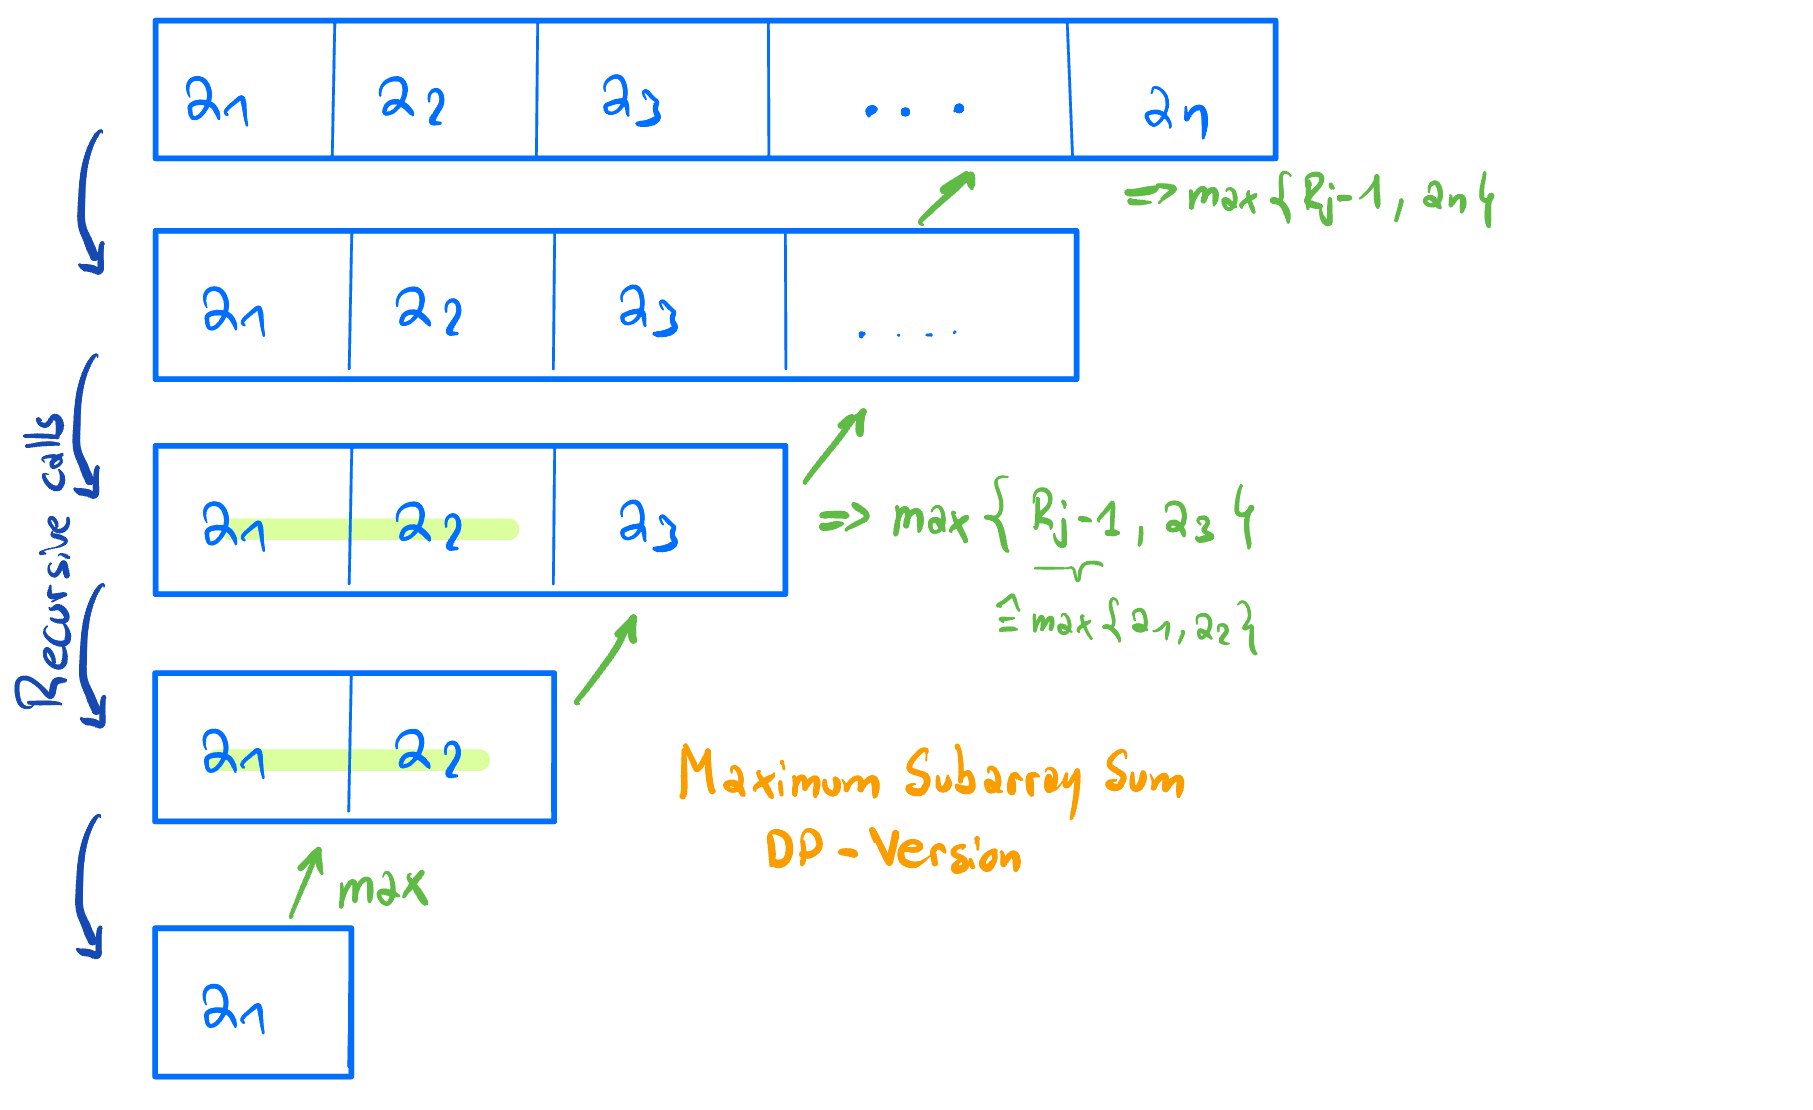
\includegraphics[width = \textwidth]{Pictures/MSS-DPVersion.jpeg}
    \caption{Wie die Rekursion aussieht}
    \label{fig:MSS-DP}
\end{figure}

\subsection{Jump Game}
Das Jump-Game ist ähnlich aufgebaut wie das MSS Problem. Wir hapen als \textbf{Input:} ein Array $A[1\dots n], \ n \in \mathbb{N}$.
Das Spiel startet in Position $1$ und dürfen von Position $i$ höchstens $A[i]$ nach vorne (auf eine beliebige Position zwischen $i+1, \dots, i+A[i]$) springen. \textbf{Gesucht:} Minimale Anzahl an Sprüngen um $n$ zu erreichen.
\subsubsection*{Erster Ansatz}
Teilproblem: $S[i] :=$ Mindestanzahl an Sprüngen um $i$ zu erreichen\\
Rekursion: $S[i] = \min\lbrace 1 + S[j] \mid 1 \leq j < i $ und "$j+ A[j] \geq i\rbrace$, wobei $j+A[j]\geq i$" =   "können $i$ von $j$ aus erreichen"

\begin{algorithm}[h]
\caption{Jump Game | Bottom-up}
 \label{alg:JumpGame-bottomUp}
\begin{algorithmic}
  \State $S[1] \gets 0$
  \For{$i = 2 \dots n$} 
    \State $S[i] \gets \infty$  \Comment{Zahl die garantiert grösser ist als Ergebnis}
    \For{$j = 1 \dots i-1$}
    \If{$j+A[j] \geq i$}
    \State $S[i] \gets \mid\lbrace S[i], 1+S[j] \rbrace$
    \EndIf
    \EndFor
 \EndFor
\State \Return $S[n]$
\end{algorithmic}
\end{algorithm}

Die Laufzeit dieses Algorithmus ist: $\Theta\big(\sum_{i=1}^n(i-1)\big) = \Theta(n^2)$
\subsubsection*{Zweiter Ansatz}
Teilproblem: $M[k] :=$ maximaler Index, den wir in $k$ Sprüngen erreichen \\
Rekursion: $M[k] \gets \max\lbrace i+A[i] \mid M[k-2] < i \leq M[k-1]\rbrace$ 

\begin{algorithm}[h]
\caption{Jump Game zweiter Ansatz| Bottom-up}
 \label{alg:JumpGame2-bottomUp}
\begin{algorithmic}
  \State $k \gets 0$
  \State $M[0] \gets 1$
  \State $M[-1] \gets 0$
  \While{$M[k] < n$}
    \State $l \gets k+1$
    \State $M[k] \gets \max\lbrace i+A[i] \mid M[k-2] < i \leq M[k-1]\rbrace$ 
    \EndWhile
\State \Return $k$
\end{algorithmic}
\end{algorithm}
Die Laufzeit dieses Algorithmus ist: $\mathcal{O}(n)$
Auch in $\mathcal{O}(n)$ laufender Code, der dasselbe Ergebnis liefert:

\begin{lstlisting}[language = Java , commentstyle=\color{teal}]
public int jump(int[] nums) {
    // The starting range of the first jump is [0, 0]
    int answer = 0, n = nums.length;
    int curEnd = 0, curFar = 0;
        
    for (int i = 0; i < n - 1; ++i) {
        // Update the farthest reachable index of this jump.
        curFar = Math.max(curFar, i + nums[i]);
            
        // If we finish the starting range of this jump,
        // Move on to the starting range of the next jump.
        if (i == curEnd) {

            answer++;
            curEnd = curFar;
        }
    }
    return answer;
}
\end{lstlisting}


\subsection{Längste gemeinsame Teilfolge}
Was ist die LGT von \texttt{SEMESTER} $= A[1\dots n]$ und \texttt{VERBESSERN} $= B[1\dots m]$? Diese lautet \texttt{EESER}.
Wir wollen in diesem Abschnitt eine Teilfolge finden, die die LGT sucht. Lücken zwischen den einzelnen Buchstaben ist egal, dafür muss die Reihenfolge stimmen. Wir formulieren wieder unser Teilproblem und dessen dazugehörige Rekrusion:\\
Teilproblem : für alle $i,j$ Wie gross ist $L(i,j) :=$ Länge eines LGT von $A[1\dots i]$ und $B[1\dots j]$ ?
Rekursion: $i = 0$ oder $j = 0 \implies L(i,j) = 0$, wenn $i,j > 0$   folgt:
\begin{enumerate}
    \item Möglichkeit: Verwende $A[i]$ und $B[j]$. Geht nur wenn $A[i] = B[i]$
    \item Möglichkeit: Verwende $A[i]$ und nicht $B[j]$.
    \item Möglichkeit: Verwende $A[i]$ nicht, dafür $B[j]$.
\end{enumerate}
$\rightarrow$ Falls  $A[i] = B[j]$, dann $L(i,j) = \max\lbrace 1 + L(i-1, j-1), L(i-1, j), L(i, j-1) \rbrace$ \\
$\rightarrow$ Falls  $A[i] \neq B[j]$, dann $L(i,j) = \max\lbrace L(i-1, j), L(i, j-1) \rbrace$

Zur Berechnung nutzen wir eine \textbf{DP-Tabelle}. In diesem Programm steht die LGT zum Zeitpunkt $L(i,j)$
Wir gehen diesen Prozess einmal durch. Man soll bedenken wenn $A[i] = B[i]$, nehmen wir das in der DP-Tabelle stehende $L(i-1,j-1)$-te Element addieren $+1$ dazu (Vgl. blauer Pfeil Fig. \ref{fig:LGT01}) 
Die Laufzeit dieses Algorithmus \& dessen benötigten Speicher ist $\mathcal{O}(nm)$.

\begin{lstlisting}[language = Java , commentstyle=\color{teal}]
public int LGT(String X, String Y, int m, int n, int[][] dp) {
     if (m == 0 || n == 0) return 0; //dp[][] initial to -1
     if (dp[m][n] != -1) return dp[m][n]; //we have already calculated value
     if (X.charAt(m - 1) == Y.charAt(n - 1)) {
        dp[m][n] = 1 + LGT(X, Y, m - 1, n - 1, dp);
         return dp[m][n];
     }
        dp[m][n] = Math.max(LGT(X, Y, m, n - 1, dp), LGT(X, Y, m - 1, n, dp));
        return dp[m][n];
}
\end{lstlisting}

\begin{figure}[h]
\centering
\begin{subfigure}{0.45\textwidth}
    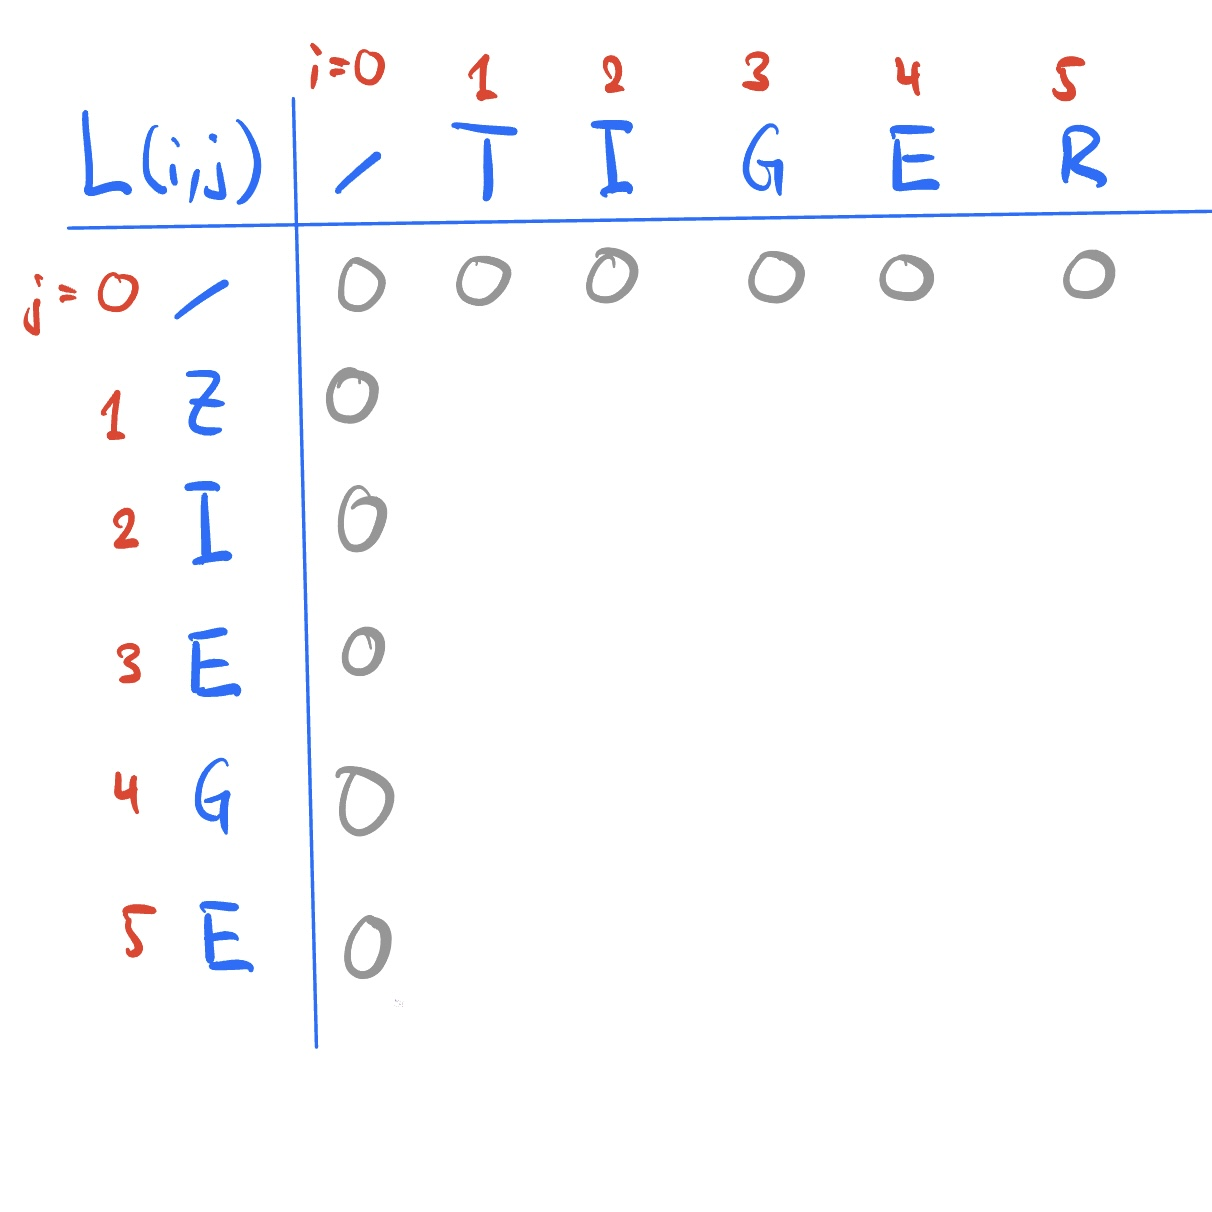
\includegraphics[width=\textwidth]{Pictures/LGT0.jpg}
        \caption{"Base Case"}
        \label{fig:LGT00}
\end{subfigure}
\hfill
\begin{subfigure}{0.45\textwidth}
 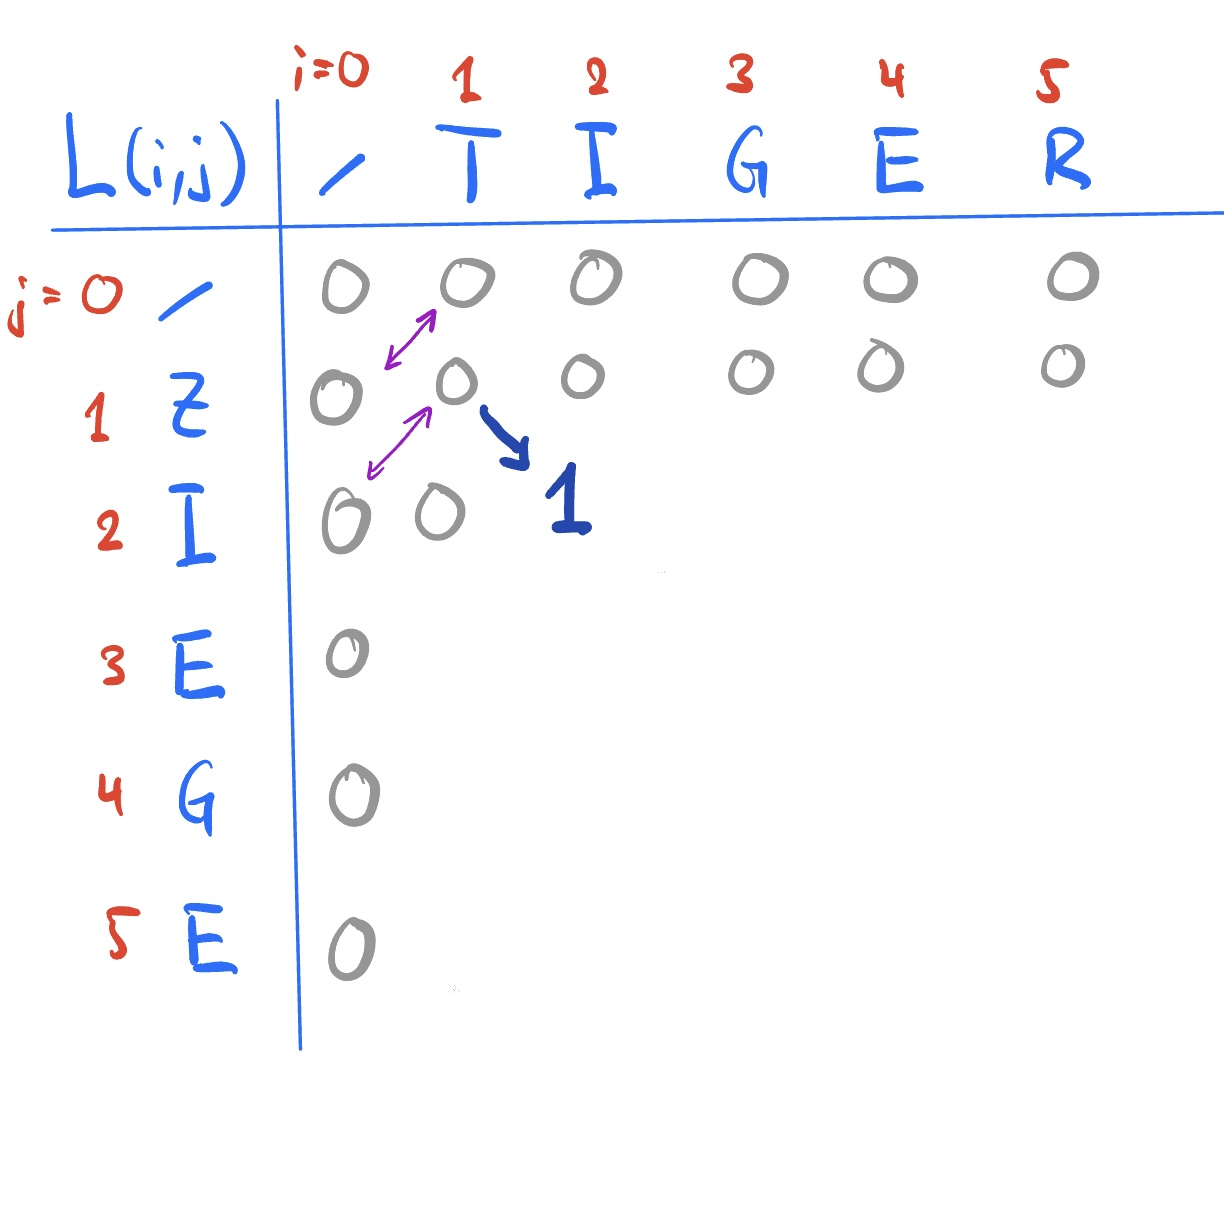
\includegraphics[width=\textwidth]{Pictures/LGT1.jpg}  
 \caption{Erste Veränderung: $A[i] = B[j]$}
        \label{fig:LGT01}
\end{subfigure}

\begin{subfigure}{0.7\textwidth}
 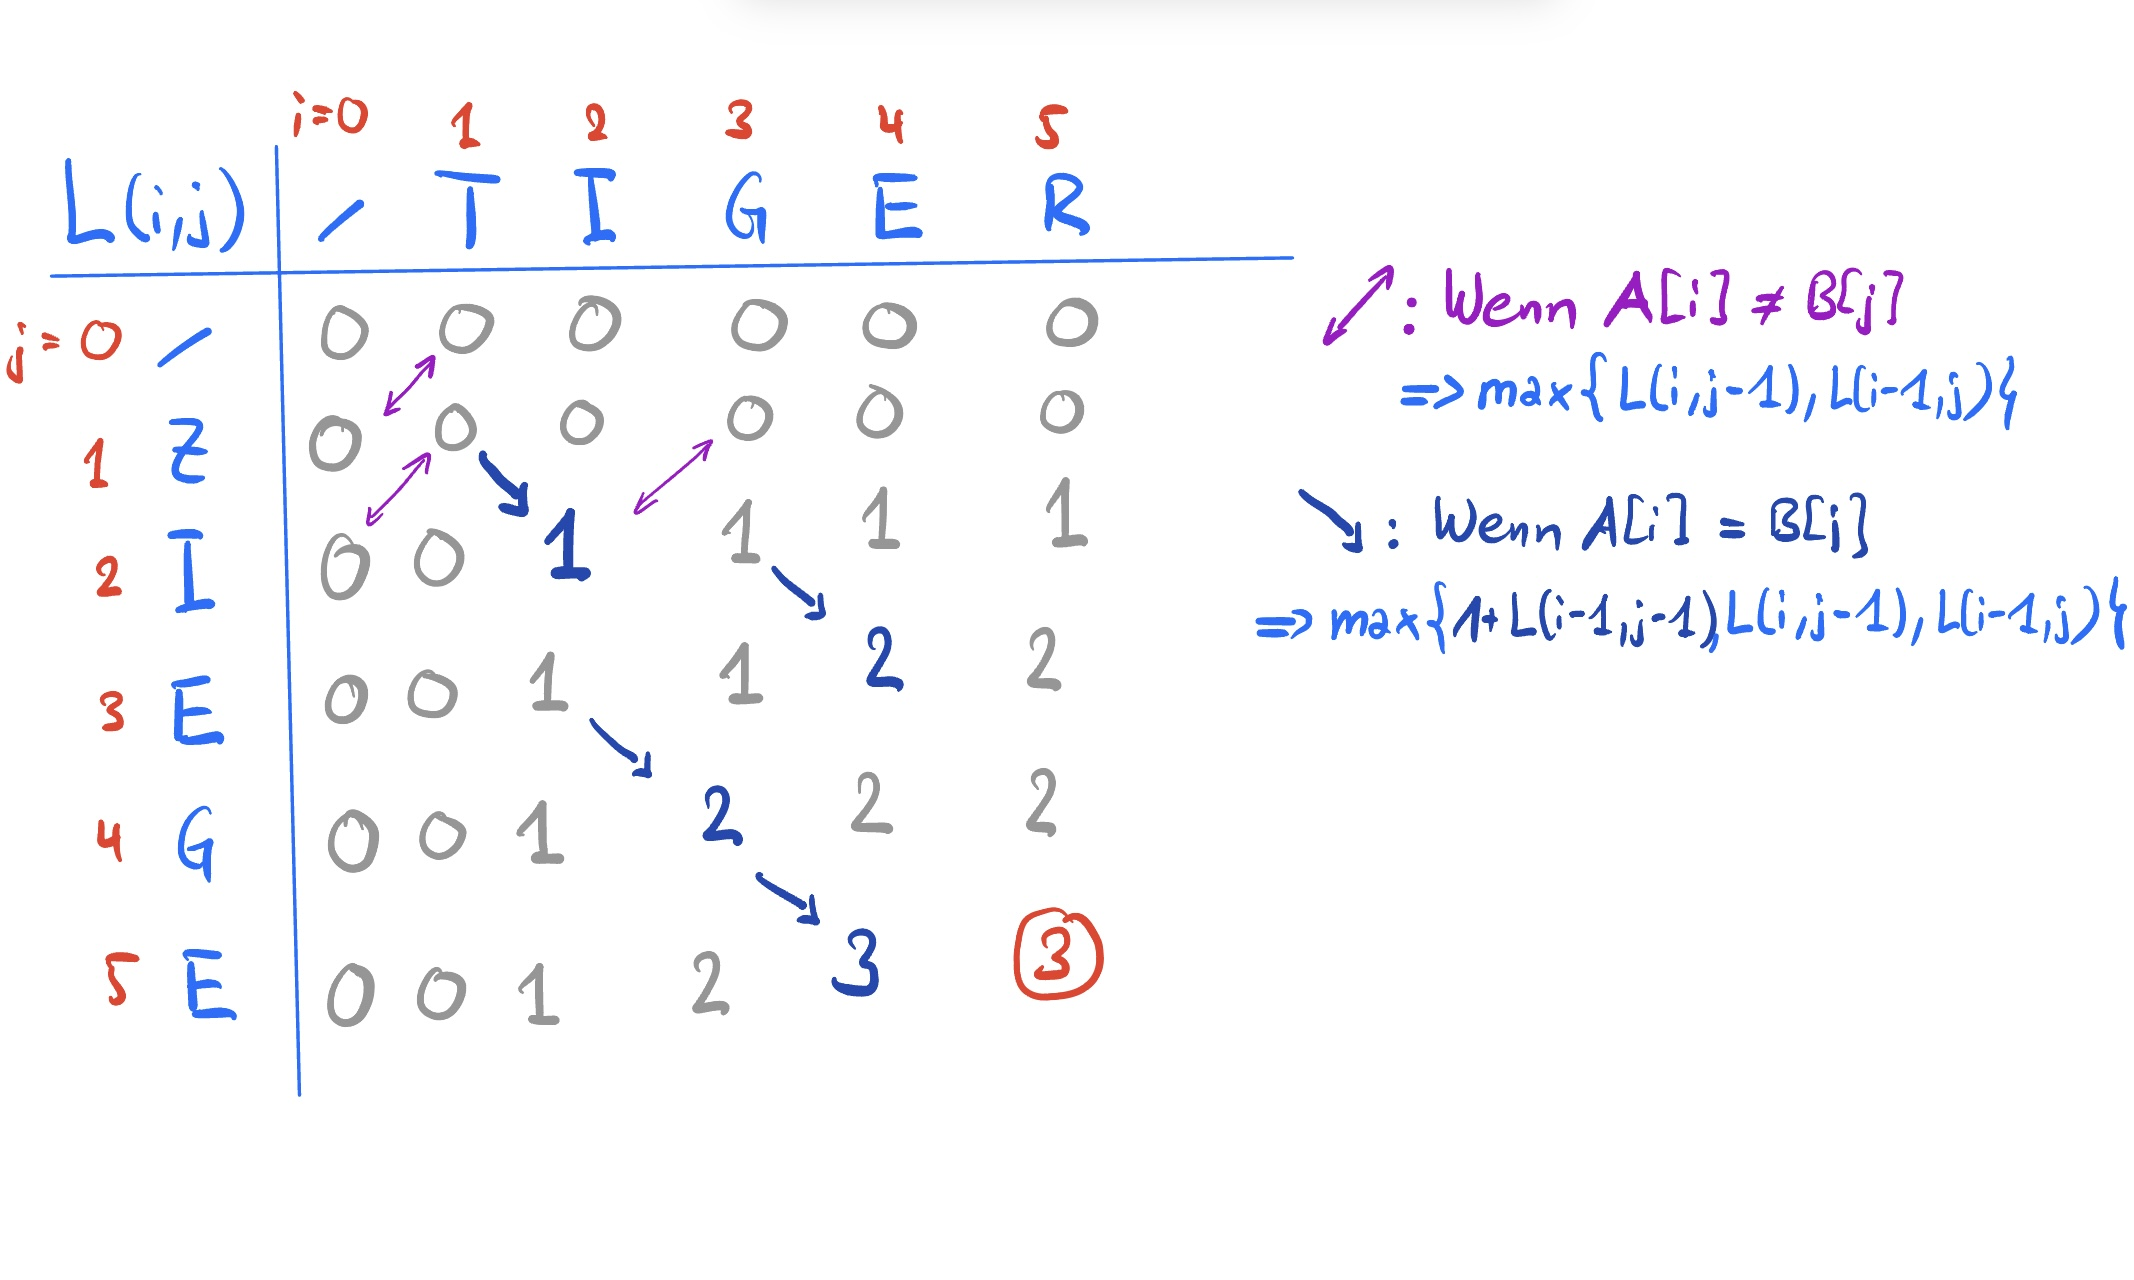
\includegraphics[width=\textwidth]{Pictures/LGT2.jpg}
        \caption{Finale DP-Tabelle}
        \label{fig:LGT02}
\end{subfigure}
\caption{LGT-Ablauf von Base case zu finaler DP-Tabelle}
\label{fig:LGT-Ablauf}
\end{figure}

\subsection{Minimale Editierdistanz}
Was ist die minimale Editierdistanz von \textsc{TIGER} $= A[1\dots n]$ und \textsc{ZIEGE} $= B[1\dots m]$, sodass $String(A) = String(B)$ ?
Die Operationen die benötigt werden dürfen für dieses Problem sind:
\begin{itemize}
    \item \texttt{ändern}: TIGER $\rightarrow$ ZIGER
    \item \texttt{einfügen}: TIGER $\rightarrow$ ZIEGER
    \item \texttt{löschen}: TIGER $\rightarrow$ ZIEGE    
\end{itemize}

Teilproblem: $ED(i, j) :=$ [Edits von $A[1\dots i] nach B[1\dots j]$] \\

Fallunterscheidung:
\begin{enumerate}
    \item Fall: $A[i]$ gelöscht $\rightarrow$ kann man gleich machen $\implies ED(i, j) = 1 + ED(i-1, j)$ 
    \item Fall: $A[i]$ am Ende auf ein Element von $B[1\dots j-1]$ gematcht. $\implies B[j]$ muss irgendwann eingefügt werden $\rightarrow$ kann man direkt machen $\implies ED(i, j) = 1 + ED(i, j)-1$
    \item Fall: $A[i]$ wird auf B[j] gematcht. 
    \begin{equation*}
    \implies ED(i, j)  =
        \begin{cases*}
           $ ED(i-1, j-1)$ &  falls $ A[i] = B[j] $\\
           $ 1 + ED(i-1, j-1)$ &  falls $ A[i] \neq B[i]$ 
        \end{cases*}
    \end{equation*}
\end{enumerate}



\begin{equation*}
    \text{Als Base case haben wir:}
  \begin{cases}
    ED(i, 0) = i & \text{erste Spalte}  \\
    ED(0, j) = j & \text{erste Zeile}
    \end{cases}   
\end{equation*}

\textbf{Für $i, j > 0$: }
\begin{equation*}
    {ED}(i, j) = \min \left( \begin{array}{c}
    {ED}(i-1, j) + 1 \text{ (A[i] löschen)}\\
    {ED}(i, j-1) + 1 \text{ (B[i] einfügen)}\\
    {ED}(i-1, j-1) + \begin{cases}
    0 & \text{if } A[i] = B[j] \\
    1 & \text{if } A[i] \neq B[j] \text{ (A[i] durch B[j] ersetzen)}
    \end{cases} \\
    \end{array} \right)
\end{equation*}


Durchspielen eines Beispieles:
\begin{figure}[h]
\centering
\begin{subfigure}{0.45\textwidth}
    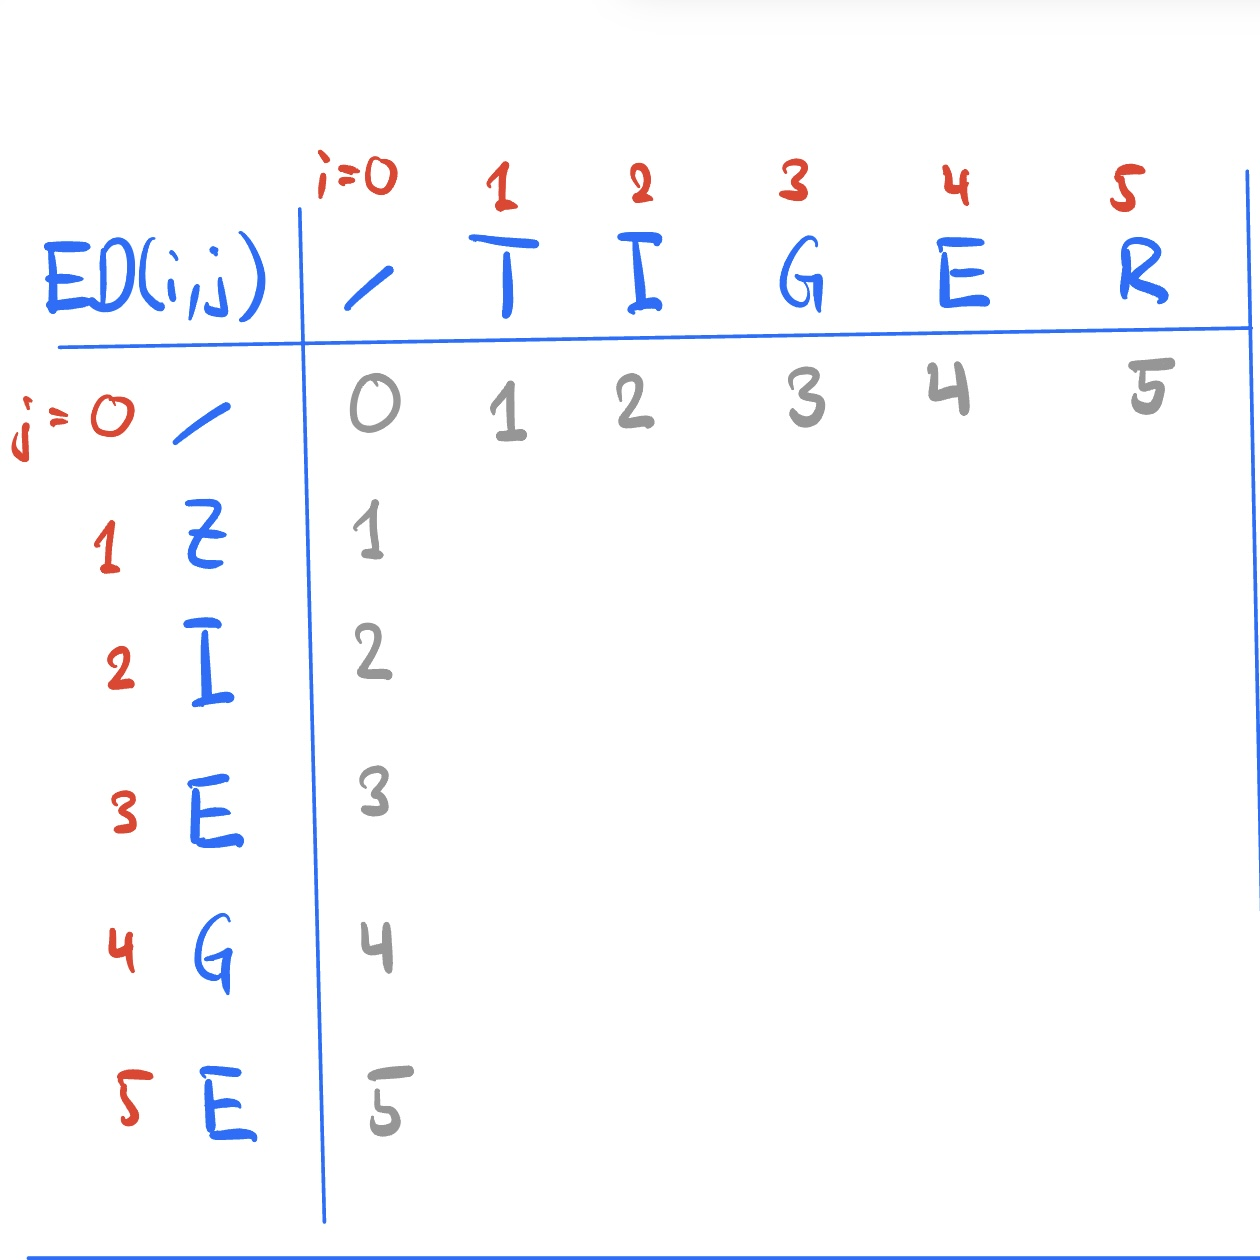
\includegraphics[width=\textwidth]{Pictures/ED0.jpg}
        \caption{"Base Case"}
        \label{fig:ED00}
\end{subfigure}
\hfill
\begin{subfigure}{0.45\textwidth}
 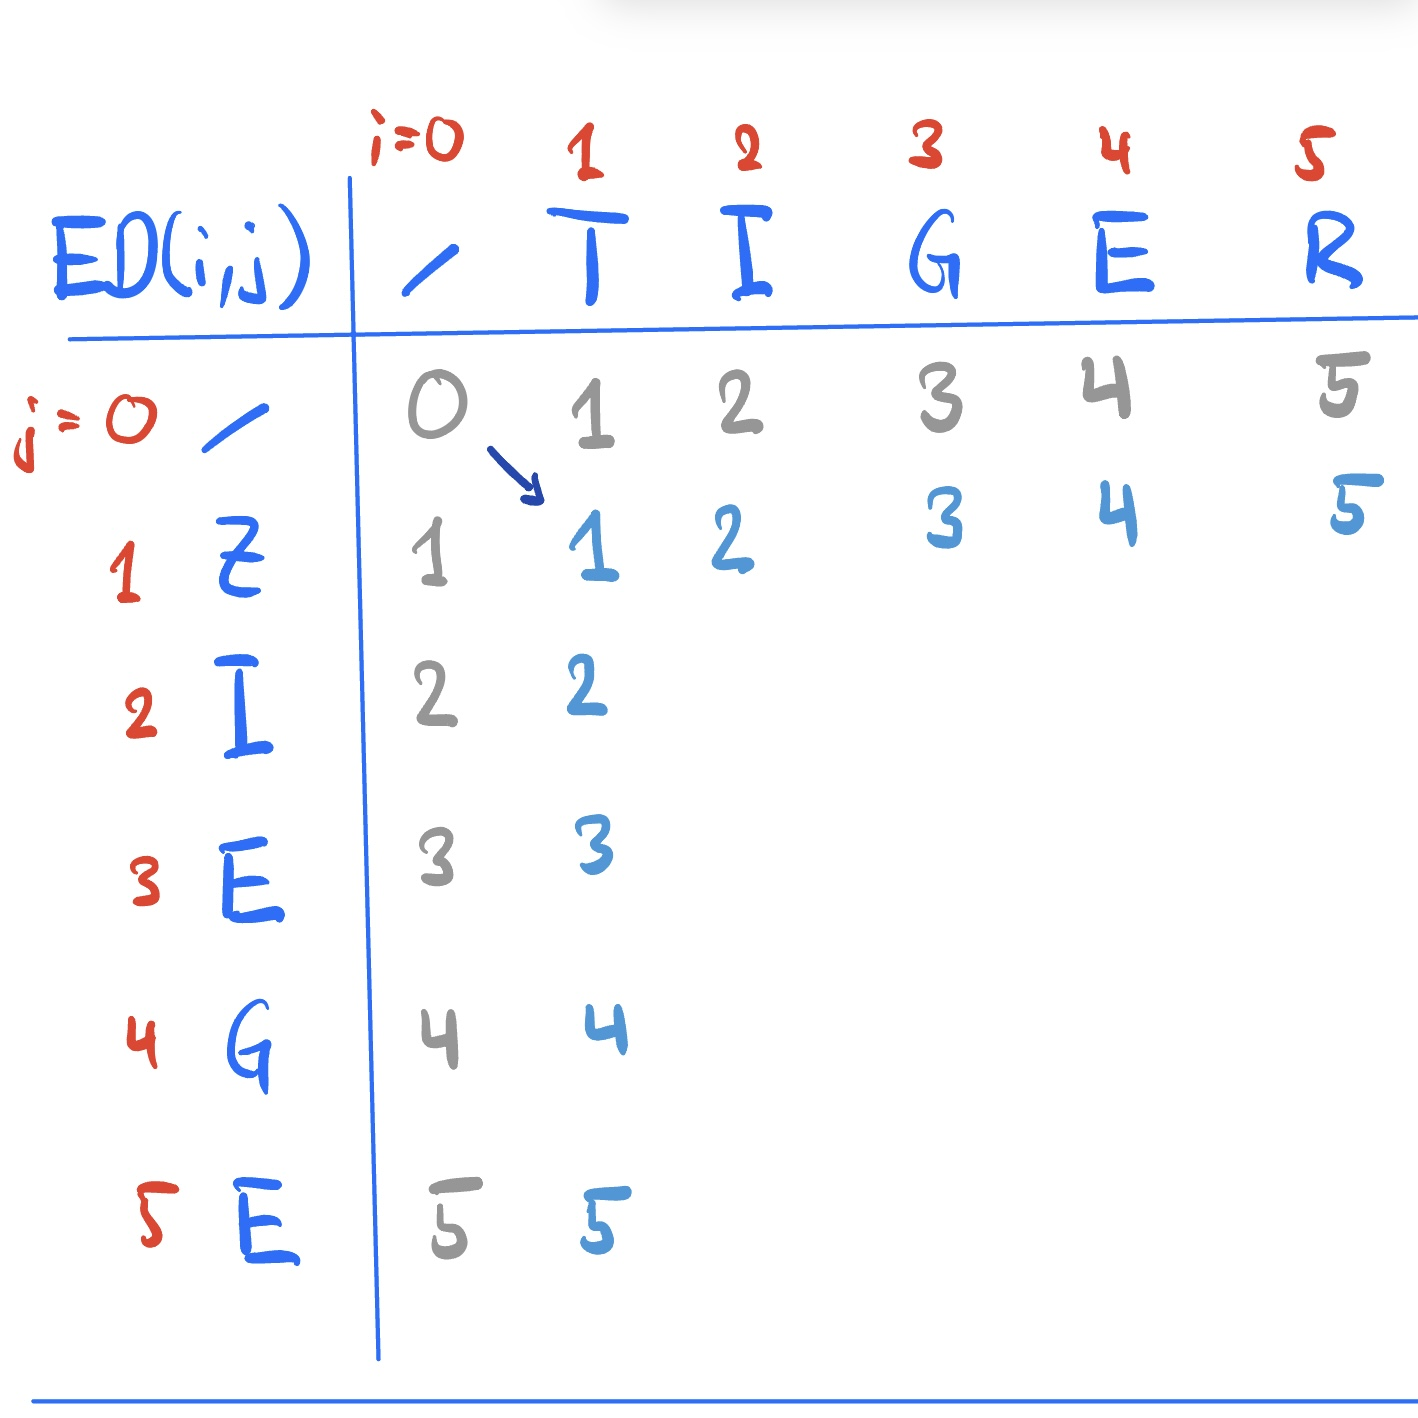
\includegraphics[width=\textwidth]{Pictures/ED1.jpg}  
 \caption{Case $ED(j-1, j-1) + 1$, da $A[i] \neq B[j]$}
        \label{fig:ED01}
\end{subfigure}

\begin{subfigure}{0.45\textwidth}
 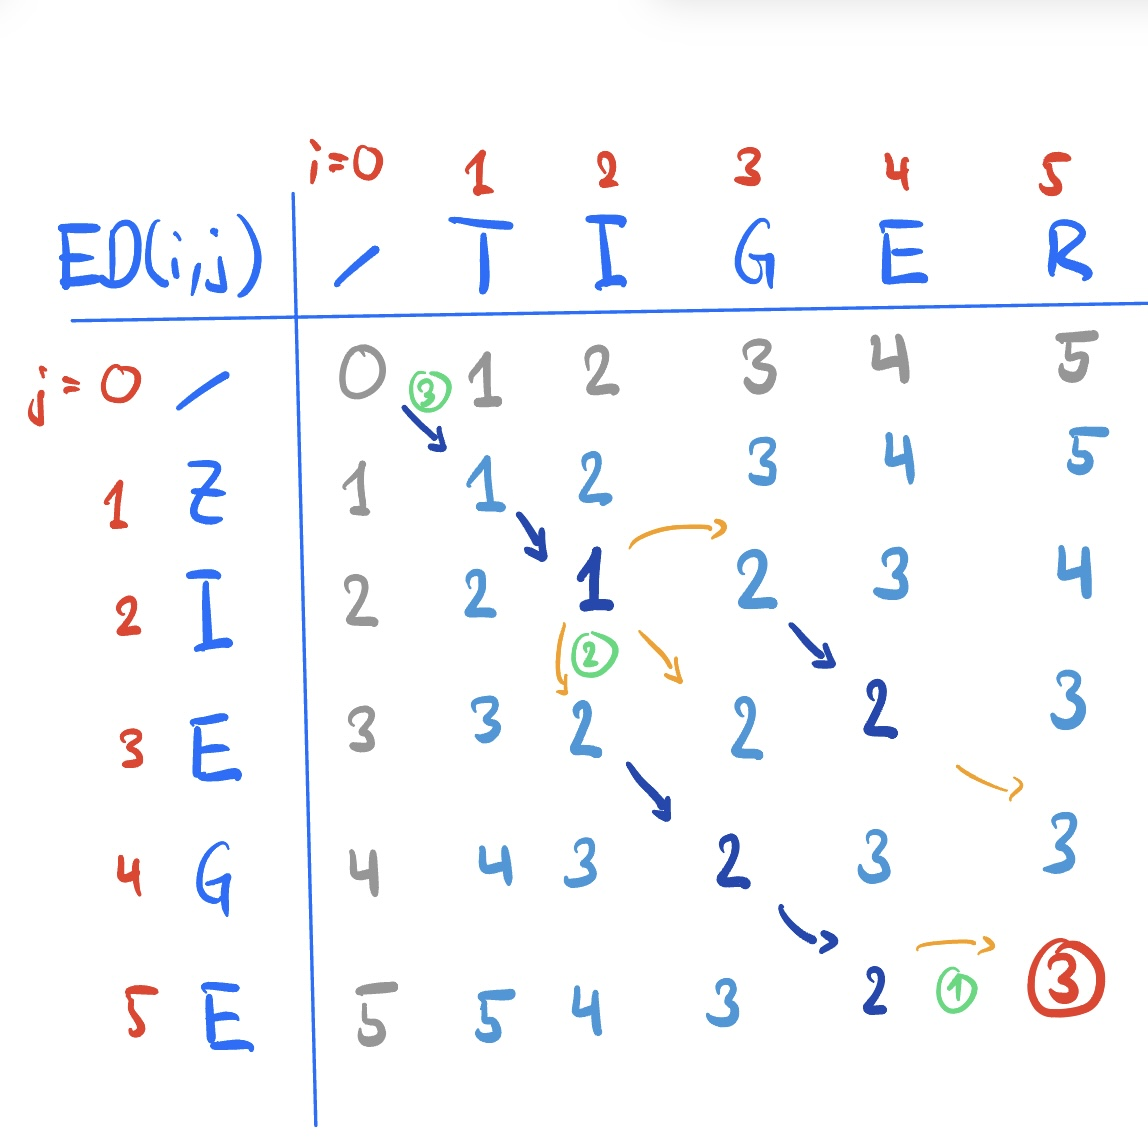
\includegraphics[width=\textwidth]{Pictures/ED2.jpg}
        \caption{Finale DP-Tabelle}
        \label{fig:ED02}
\end{subfigure}
\begin{subfigure}{0.45\textwidth}
 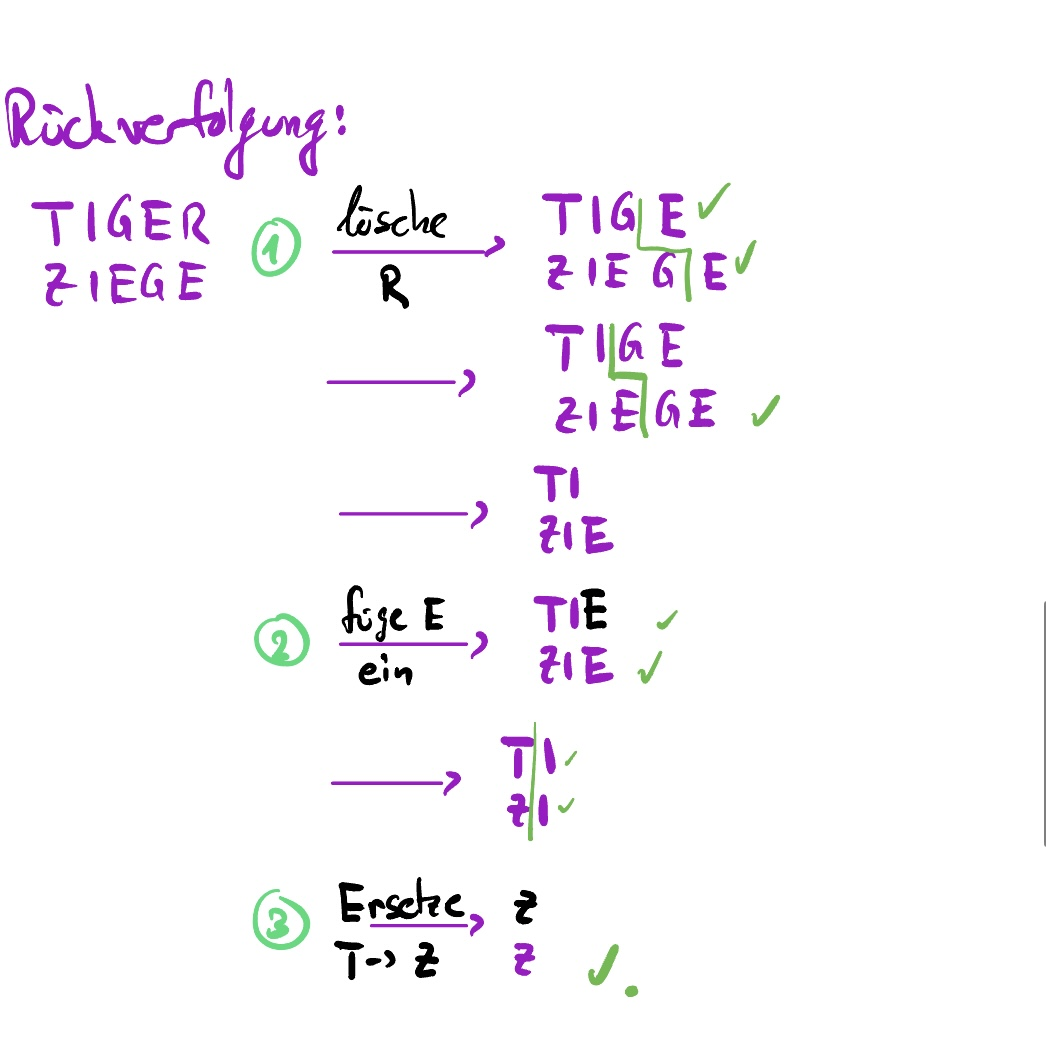
\includegraphics[width=\textwidth]{Pictures/ED3.jpg}
        \caption{Rückverfolgung von Figure(\ref{fig:ED02})}
        \label{fig:ED03}
\end{subfigure}
\caption{ED-Ablauf von Base case zu finaler DP-Tabelle mit Rückverfolgung}
\label{fig:ED-Ablauf}
\end{figure}

Die Laufzeit dieses Algorithmus \& dessen benötigten Speicher ist $\mathcal{O}(nm)$.


\subsection{Subset Sum Problem}
In diesen Problem haben wir als Input: Array $A = [1\dots n], b$, wobei alle Zahlen $\in \mathbb{N}$. Ziel dieses Problems ist, ob wir eine Teilmenge (rsp. Teilsumme) $I$ von dem Array $A$ finden können, so dass dies $b$ ergibt:
$I \subseteq \lbrace 1\dots n\rbrace$, sodass $\sum_{i\in I}A[i] = b$.
\subsubsection*{Beispiel:}
Array $A = [5, 3, 10, 3, 1]$ mit $b$, wobei für $b$ verschiedene Fälle angesehen werden:
\begin{equation*}
 b = 
    \begin{cases*}
           $ 12 $ &  \checkmark\\
           $ 2 $  &  $\lightning$ \\
           $> 22$ &  $\lightning$ \\
           $= 20$ &  $\lightning$
        \end{cases*}
\end{equation*}
Wir definieren wieder unser Teilproblem und dessen Rekursion: \\
Teilproblem : $T(i, s) :=$ "Ist $s$ eine Teilsumme von $A[1\dots i]$ ?" $\in \lbrace 0, 1 \rbrace$ (false, true) \\
Rekursion: wir haben zwei Möglichkeiten 1.) wir benutzen $A[i]$ oder 2.) wir benutzen $A[i]$ nicht. 
\begin{equation*}
    \implies T(i, s) = T(i-1, s) \lor T(i-1, s-A[i]) 
\end{equation*}
Our base cases are defined by: $ T(i, 0) = 1,\ T(0, s) = 0, s > 0$

Table for $b= 7$: 


\begin{table}[h]
\parbox{.45\linewidth}{
\centering
    \centering
    \begin{tabular}{cc|cccccccc}
        & $T(i,s)$ & 0 & 1 & 2 & 3  & 4  & 5  & 6 & 7*\\
    \hline
      i= 0 & /& 1 & 0 & 0 & 0 & 0 & 0 & 0 & 0 \\
        1 & 5 & 1 &  &  &  &  &  &\\
        2 & 3 & 1 &  &  &  &  &  &\\
        3 & 10 &1 &  &  &  &  &  &\\
        4 & 3 & 1 &  &  &  &  &  &\\
        5 & 1 & 1 &  &  &  &  &  &\\
    \end{tabular}
    \caption{Base Case | *: $b=7$}
    \label{tab:SubSetSum-Basecase}
}
\hfill
\parbox{.45\linewidth}{
\centering
    \begin{tabular}{cc|cccccccc}
        & $T(i,s)$  & 0 & 1 & 2 & 3  & 4  & 5  & 6 & 7*\\
    \hline
      i= 0 & /& 1\tikzmark{a}& 0 & 0 & 0 & 0 & 0 & 0 & 0 \\
      
        1  & 5 & 1\tikzmark{b}& \textcolor{gray}{0}  & \textcolor{gray}{0}  & \textcolor{gray}{0} & \textcolor{gray}{0} &\textcolor{red}{1}  & \textcolor{gray}{0} & \textcolor{gray}{0}\\
        
        2 & 3 & 1& \textcolor{gray}{0}  & \textcolor{gray}{0}  & \tikzmark{c}\textcolor{red}{1}  & \textcolor{gray}{0} &\textcolor{red}{1}  & \textcolor{gray}{0} & \textcolor{gray}{0}\\
        
        3 & 10 &1& \textcolor{gray}{0}  & \textcolor{gray}{0}  & \tikzmark{d}\textcolor{red}{1} & \textcolor{gray}{0} &\textcolor{red}{1}  & \textcolor{gray}{0} & \textcolor{gray}{0}\\
        
        4 & 3 & 1& \textcolor{gray}{0}  & \textcolor{gray}{0}  & \textcolor{red}{1} & \textcolor{gray}{0} &\textcolor{red}{1}  & \tikzmark{e}\textcolor{red}{1} & \textcolor{gray}{0} \\
        
        5 & 1 & 1& \textcolor{red}{1}  & \textcolor{gray}{0}  & \textcolor{red}{1} & \textcolor{red}{1} &\textcolor{red}{1}  & \textcolor{red}{1} & \tikzmark{f}\textcolor{red}{\circled{1}} \\
    \end{tabular}
    \begin{tikzpicture}[overlay, remember picture, shorten >=.5pt, shorten <=.5pt, transform canvas={yshift=.25\baselineskip}, color = teal]

    \draw [<-] ([yshift=.75pt]{pic cs:a}) -- ({pic cs:b});
    \draw [<-] ([yshift=.75pt]{pic cs:b}) -- ({pic cs:c});
    \draw [<-] ([yshift=.75pt]{pic cs:c}) -- ({pic cs:d});
    \draw [<-] ([yshift=.75pt]{pic cs:d}) -- ({pic cs:e});  \draw [<-] ([yshift=.75pt]{pic cs:e}) -- ({pic cs:f});
  \end{tikzpicture}
    \caption{Fully developed table with \textcolor{teal}{backtracking} }
    \label{tab:SubSetSum-FinishedTable}
    }
\end{table}
Die Lösung dieses Problems ist mit \textcolor{red}{\circled{1}} gekennzeichnet und kann zurückverfolgt werden via $3 + 3 + 1 = 7$, wenn $T(n,b) =$ \textcolor{red}{\circled{0}}, so würde es keine Lösung für dieses Problems geben. 
Die Laufzeit dieses Algorithmus \& dessen benötigten Speicher ist $\Theta(n\cdot b)$. Da die Laufzeit nun abhänig von der Grösse einer Zahl ist \textbf{pseudo-polynomiell}. \\
Es gilt: \\ 
$n$: Anzahl der Zahlen im Input \\
$b$: eine einzelne Zahl aus dem Input\\
Für $b= 2^n: $ Inputlänge $\Theta(n)$ Laufzeit: $\Theta(n\cdot2^n)$ (\textbf{exponentiell}) \\
Für $b= b^c: $ Inputlänge $\Theta(n)$ Laufzeit: $\Theta(n\cdot2^{c+1})$(\textbf{polynomiell})

\subsection{Knap Sack Problem}
Erweiterung des Subset-Sum Problems. Bei diesem Problem haben wir als \textbf{Input}: Rucksack mit Gewichtslimit $W$ und $n$ Gegenstände mit Gewicht $w_i \in \mathbb{N}$ und Wert $v_i \in \mathbb{N}, i = 1\dots n$. \textbf{Gesucht}: Teilmenge $I \subseteq \lbrace 1,\dots ,n \rbrace$ sodass $\sum_{i\in I} w_i \leq W$ und $\sum_{i\in I} v_i$ maximal. \\ 
\textbf{Ansätze:} 
\begin{enumerate}
    \item alle $I$ ausprobieren $\rightarrow 2^n$ Möglichkeiten $\rightarrow$ zu teuer.
    \item Greedy-Algorithmen: Nimm zuerst Element 
    \begin{enumerate}
        \item mit grösstem Wert
        \item mit kleinstem Wert
        \item mit bestem Preis-Leistung Verhältnis: $v_i /w_i$
    \end{enumerate}
\end{enumerate}
Jedoch liefert dieser Ansatz kein korrektes Ereignis:f

\begin{equation*}
    (v_1,w_1) = (v_2,w_2) = (2,2) ; (v_3,w_3) = (3,3) ; w = 4
\end{equation*}
$\rightarrow I = \lbrace 1,2\rbrace$ ist optimal, aber a) nimmt $I = \lbrace 3\rbrace$ an.
\begin{equation*}
    (v_1,w_1) = (1,1) ; (v_2,w_2) = (9,10) ; w = 10
\end{equation*}
$\rightarrow I = \lbrace 2\rbrace$ ist optimal, aber b) und c) nehmen $I = \lbrace 1\rbrace$ an.
\subsubsection*{DP-Teilproblem:} $MW(i, w) :=$ maximaler Wert, den man aus $1 \dots n$ mit Höchstgewicht $w$ erreichen kann. \\
\textbf{Rekursion:} $MW(i,w) = \max \lbrace MW(i-1, w) , v_i + MW(i-1,w-w_i)\rbrace$, wobei 
\begin{itemize}
    \item $MW(i-1, w) :=$ verwende item $i$ nicht
    \item $v_i + MW(i-1,w-w_i) :=$ verwende item $i$. Nur möglich, falls $w_i \leq w$.
\end{itemize}
Tabelle:
\begin{table}[h]
    \centering
\begin{tabular}{c|ccccccccc}
  \backslashbox{i}{w} & 0 & 1 & 2 & $\dots$ & $w \cdot w_i$ & $\dots$ & $w$ &  & $W$\\
  \hline
  0 & 0  & 0  & 0  & 0  & 0 & 0 & 0 & 0 & 0\\
  1 &  0 &  & & & & & & &\tikzmark{aa}   \\
  $\vdots$ & $\vdots$  & \\
    & $\vdots$  &   &   &   &  &  &  &  \\
  $i-1$ & $\vdots$  &   &   &   & $\bullet$ \tikzmark{cc} &  & $\bullet$\tikzmark{dd} &  \\
  $i$ & $\vdots$  &   &   &   &  &  & $\bullet$\tikzmark{ee} &  \\
  $\vdots$ & $\vdots$   \\
  0 &  0 &  & & & & & & &\tikzmark{bb}   \\ 
  $n$ & 0  & \tikzmark{ff}  &   &   &  &  &  & \tikzmark{gg} & \textcolor{red}{$\bullet$}  \\
  \hline
\end{tabular}
  \label{tab:KnapSackV1}
  \caption{Fully developed table with \textcolor{red}{backtracking} }
  \begin{tikzpicture}[overlay, remember picture,shorten >=.5pt, color = red]
    \draw [-] ({pic cs:aa}) -- ({pic cs:bb});
    \draw [-] ({pic cs:ff}) -- ({pic cs:gg});
    \draw [->] ({pic cs:cc}) -- ({pic cs:ee});
    \draw [->] ({pic cs:dd}) -- ({pic cs:ee});
  \end{tikzpicture}
\end{table}
Der Punkt: \textcolor{red}{$\bullet$}, ist die Lösung dieses DP-Tables.
Die Laufzeit dieses Algorithmus und dessen benötigten Speicher ist $\mathcal{O}(nW)$ (\textbf{pseudo-polynomiell}).

\subsubsection*{Alternativ-DP:} 
\textbf{Teilproblem:} $MG(i, v) :=$ minimales Gewicht, das man braucht, um aus$1 \dots i$ einen Wert $\geq v$ zu erzeugen ($MG(i, v) = \infty)$, wenn $v$ gar nicht erreicht werden kann \\
\textbf{Rekursion:} $MG(i,v)= \min\lbrace MG(i-1, v), w_i + MG(i-1, v-v_1)\rbrace$ ($MG(i-1, v-v_1) = 0$, falls $v_i \geq v$)

\begin{table}[h]
\centering
\begin{tabular}{c|ccccccccccc}
  \backslashbox{i}{v} & 0 & 1 & 2 & $\dots$ & $v - v_i$ & $\dots$ & $v$ &  & \textcolor{red}{$\circled{}$} & $\dots$ & $V$\\
  \hline
  0 &   &   &   &   &  &  &  &  &\tikzmark{a1}  \\
  1 &  0 &  & & & & & & &  \\
  $\vdots$ &   & \\
    &   &   &   &   &  &  &  &  \\
  $i-1$ &   &   &   &   & $\bullet$ \tikzmark{c1} &  & $\bullet$\tikzmark{d1} &  \\
  $i$ &   &   &   &   &  &  & $\bullet$\tikzmark{e1} &  \\
  \\
   &   &  & & & & & & &\tikzmark{b1}   \\ 
  $n$ &  \tikzmark{f1} & &   &   &  &  &  & \tikzmark{g1} & \textcolor{red}{$\circled{}$}  \\
  \hline
\end{tabular}
  \label{tab:KnapSackV2}
  \caption{Fully developed table with \textcolor{red}{backtracking} }
  \begin{tikzpicture}[overlay, remember picture,shorten >=.5pt, color = red]
    \draw [<-] ({pic cs:a1}) -- ({pic cs:b1});
    \draw [-] ({pic cs:f1}) -- ({pic cs:g1});
    \draw [->] ({pic cs:c1}) -- ({pic cs:e1});
    \draw [->] ({pic cs:d1}) -- ({pic cs:e1});
  \end{tikzpicture}
\end{table}
Der in der ersten Zeile enthaltene \textcolor{red}{$\circled{}$}, ist die Lösung dieser DP-Tabelle. 
Der unterste enthaltene \text{\textcolor{red}{$\circled{}$}} , ist als "Suche $W$ (bzw. nächstkleineres, falls W nicht vorkommt)" definiert. Die Laufzeit dieses Algorithmus ist $\mathcal{O}(nV)$.

\subsubsection*{Weiteres über Subset Sum und NP P}
Das Subset Sum Problem ist ein Entscheidungsproblem: Antwort ja oder nein; Wir definieren: \\
$P :=$ Menge aller Entscheidungsprobleme, die in polynomieller Zeit lösbar sind \\
$NP :=$ Menge aller Entscheidungsprobleme, bei denen man im JA-Fall eine Lösung in polynomieller Zeit überprüfen kann.

\subsubsection{Approximationsalgorithmus für das KnapSack-Problem}
\textbf{Input}: $w_i, v_i, W$,\textbf{Annahme}: alle $w_i \leq W$ (sonst entferne alle Gegenstände mit $w_i > W$, passen sowieso nicht $\rightarrow V_{ips} \geq v_{max} (=\max v_i)$\\
Ziel: Lösung, die fast optimal ist in polynomieller Zeit zu finden. $\implies$ Der ganze Beweis ist unter \href{https://cadmo.ethz.ch/education/lectures/HS23/DA/lectures/AD23-08.pdf}{Beweis des Approximationsalgorithmus für das Rucksackproblem} zu finden.

\subsection{Longest Ascending Subsequence}
\textbf{Input:} Array $A[1\dots n]$ von Integers. \textbf{Annahme}: keine Zahl kommt doppelt vor und \textbf{Gesucht:} Länge der längsten aufsteigenden Teilfolge $LAT$ (Reihenfolge muss gleich bleiben, aber Lücken sind erlaubt).
\subsubsection*{Beispiel}:
$A =  [2, 13, 17, 9, 11, 4, 78, 28, 15, 25, 99] \implies LAT = 2, 9, 11, 15, 25, 99;$ 
\subsubsection*{Lösung mit DP:}
Versuch 1: $LAT(i):=$ längste aufsteigende Teilfolge (AT) von $A[1\dots i] \rightarrow \lightning$ \\
Versuch 2: Merke alle Endungen einer $LAT$ in $A[1\dots i] \rightarrow \lightning$\\
Versuch 3: Merke auch kürzere AT in $A[1\dots i] :$
\begin{center}
$E(i,l):=$ "Es gibt AT der Länge l, die in i endet"$\in \lbrace 0,1\rbrace$ 
\end{center}
\textbf{Rekursion} für $l \geq 2$: 
\begin{equation*}
E(i,l) = 
    \begin{cases}
        $1$ & \text{ falls es } $j < i$\text{ gibt mit }$E(j,l-1) = 1$\text{ und }$A[j] < A[i]$ \\
        $0$ & \text{sonst}
    \end{cases}
\end{equation*}
Es folgt, dass $E(i,1) = 1$ für alle $i \in \lbrace1, \dots , n\rbrace$\\
Laufzeit: $\mathcal{O}(\sum_{l = 1}^{n}\sum_{i = 1}^{n} (i-1) = \mathcal{O}(\sum_{l=1} \frac{n(n-1)}{2}) = \mathcal{O}(n^3)$ \\
Versuch 4: $M(i,l) := $ kleinstmögliche Endung einer AT der Länge $l$ in $A[1 \dots i] \ (\inf$ falls keine solche AT existiert) \\
\textbf{Rekursion} für $i \geq 2$: 
\begin{equation*}
M(i,l) = 
    \begin{cases}
        $A[i]$ & \text{ falls } $M(i-1, l-1) < A[i] < M(i-1,l)$ \\
        $M(i-1,l)$ & \text{sonst}
    \end{cases}
\end{equation*}
\begin{equation*}
i = 1: \ M(1,l) = 
    \begin{cases}
        $A[i]$ & $l = 1$ \\
        $+\infty$ & \text{sonst}
    \end{cases}
\end{equation*}
\begin{center}
$\implies \mathcal{O}(n^2)$    
\end{center}

\subsubsection*{Beispiel $A = 3, 7, 8, 4, 5$ }
\begin{table}[h]
\parbox{.45\linewidth}{
\centering
    \centering
    \begin{tabular}{c|ccccc}
     \backslashbox{i}{l} & 1 & 2 & 3 & 4 & 5 \\
     \hline
      1 & 3 & \infty & \infty & \infty & \infty\\
      2 & 3 & \infty & \infty & \infty & \infty\\
      3 & 3 & \infty & \infty & \infty & \infty\\
      4 & 3 & \infty & \infty & \infty & \infty\\
      5 & 3 & \infty & \infty & \infty & \infty\\
    \end{tabular}
    \caption{Base Case der LAS}
    \label{tab:LAS-BaseCase}
}
\hfill
\parbox{.45\linewidth}{
\centering
    \begin{tabular}{c|ccccc}
     \backslashbox{i}{l} & 1 & 2 & 3 & 4 & 5 \\
     \hline
      1 & 3\tikzmark{A} &  \tikzmark{B}\infty & \infty & \infty & \infty\\
      2 & 3 & \tikzmark{C}\textcolor{red}{7}\tikzmark{C1} & \infty\tikzmark{D} & \infty & \infty\\
      3 & 3\tikzmark{F} & \textcolor{red}{7}\tikzmark{G} & \tikzmark{E}\textcolor{red}{8} \tikzmark{E1} & \infty & \infty\\
      4 & 3 & \tikzmark{H}\textcolor{red}{4}\tikzmark{H1} & \textcolor{red}{8}\tikzmark{I} & \infty & \infty\\
      5 & 3 & \textcolor{red}{4} & \tikzmark{J}\textcolor{red}{5}\tikzmark{J1} & \infty & \infty\\
    \end{tabular}
    \begin{tikzpicture}[overlay, remember picture,shorten >=.5pt, color = red]
    \draw [<-] ({pic cs:A}) -- ({pic cs:C});
    \draw [<-] ({pic cs:B}) -- ({pic cs:C});
    
    \draw [<-] ({pic cs:C1}) -- ({pic cs:E});
    \draw [<-] ({pic cs:D}) -- ({pic cs:E1});
    \draw [<-] ({pic cs:F}) -- ({pic cs:H});  
    \draw [<-] ({pic cs:G}) -- ({pic cs:H1});
    \draw [<-] ({pic cs:H1}) -- ({pic cs:J});
    \draw [<-] ({pic cs:I}) -- ({pic cs:J1});

  \end{tikzpicture}
    \caption{Fertige Tabelle der LAS}
    \label{tab:LAS-Finished}
}
\end{table}
Beobachtungen zu Table \ref{tab:LAS-Finished}: 
\begin{itemize}
    \item Zeilen sind sortiert
    \item Wir ändern pro Zeile nur einen Eintrag
    \item Diesen können wir mit binärer Suche in Zeit $\mathcal{O}(\log n)$ finden
    \item Wenn wir dasselbe Array für jede Zeile wiederverwenden, dauert das Update pro Zeile nur $\mathcal{O}(\log n)$
    \item insgesamt Laufzeit: $\mathcal{O}(n\log n)$
\end{itemize}
Wir machen ein zweites Beispiel: $A = [2, 13, 17, 9, 11, 4, 28, 15, 25, 99]$



\begin{table}[h]
    \centering
    \begin{tabular}{c|cccccc}
        $l$ & 1 & 2 & 3 & 4 & 5 & 6\\
        \hline
        $M(*,l) $ & $\circled{2}$ & 13 & 17  & 78 & $\circled{25}$ & $\circled{99}$\\
         &  & $\circled{9}$ & $\circled{11}$ &  28 & &   \\
         &  & 4 &  &  $\circled{15}$ &  & \\
    \end{tabular}
    \caption{LAS-optimiert}
    \label{tab:LAS-final}
\end{table}

Mithilfe der Rückverfolgung die LAT ist wie folgt aufgebaut: $99 \rightarrow 25 \rightarrow 15 \rightarrow 11 \rightarrow 9 \rightarrow 2$. Es folgt zusätzlich, dass der Extraspeicher $\mathcal{O}(n)$ ist und die Laufzeit sich auf $\mathcal{O}(n\log n)$ beschränkt.


\subsection{Matrixkettenmultiplikation}
Problem: Berechne Matrizenprodukt $A_1\cdot A_2\cdot _{...}  \cdot A_n$ so günstig wie möglich: $A_i$ ist eine $k_i \times l_i$-Matrix, $k_i, l_i \in \mathbb{N}, k_{i-1} = l_1$, so dass das Produkt sinnvoll ist. \\
Freiheitsgrad: Assoziativität $\big((A_1 \cdot A_2) \cdot A_3 = A_1 \cdot (A_2 \cdot A_3) \big) $ \\
Teilproblem: $M(i,j):=$ minimale Zahl an Operationen zur Berechnung von $A_i\cdot _{...} \cdot A_j, i \leq j$ \\
Rekursion: $(A_i\cdot A_{i+1}\cdot _{...} \cdot A_s) \cdot (A_{s+1}\cdot _{...}  \cdot A_j)$,
wobei der erste Teil $k_i \times l_s$ entspricht, die

Multiplikation zwischen den beiden Klammern die letzte Multiplikation repräsentiert und der letzte Teil $k_{s+1} \times l_j = l_s \times l_j$ repräsentiert.
\begin{equation*}
    j > i: M(i,j) := \min_{i \leq s < j}\lbrace M(i,s) + M(s+1,j) + \text{Zahl Ops zur Multiplikation einer }k_i\times l_s \text{ mit einer } l_s\times l_j \text{-Matrize}\rbrace 
\end{equation*}
\begin{equation*}
        j = i: M(i,i) = 0    
\end{equation*}
Berechnungsreihenfolge: von kurzen \textit{(kleines $j-i$)} zu langen \textit{(grosses $j-i$)} Produkten, aber Diagonale weg:

\begin{figure}[h]
    \centering
    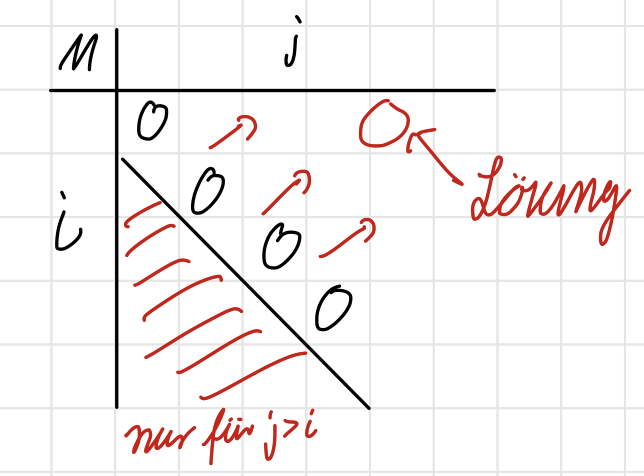
\includegraphics[width = 0.5\textwidth]{Pictures/Matrixketten.png}
    \caption{Matrixketten-Multiplikation}
    \label{fig:Matrixketten}
\end{figure}
Laufzeit: $\Theta (\big\sum_{i=1}^n\sum_{j=i}(j-i)\big) = \Theta(n^3)$ und Speicher: $\Theta(n^3)$.



\newpage
\section{Anhang}
%%Chapter 06
\subsection{Sprachunterschiede}
Important: Do not mix languages in your exam submissions! Choose the language you are most comfortable with!

\subsubsection{Deutsch}

Das Wort \emph{Graph} hei\ss t im Genitiv/Dativ/Akkusativ Singular \emph{Graphen}, also: \emph{betrachten wir einen Graphen}, nicht *\emph{betrachten wir einen Graph}.

\subsection{English}

The singular of \emph{vertices} is \emph{vertex}, not *\emph{vertice} (the Italian word for `summit').

German \emph{Kreis} = English \emph{cycle}; German \emph{Zyklus} = English \emph{circuit}.

Forms of the relative pronoun \emph{who}: \emph{who} (Nom.), \emph{whom} (Dat./Akk.), \emph{whose} (Gen.). The relative pronoun \emph{who} is only used for people, not for objects, for which you should use \emph{that} or \emph{which}.

Distinguish between the noun \emph{half} (pl. \emph{halves}) (\textcolor{blue}{Hälfte, -n}) and the verb \emph{to halve} (\textcolor{blue}{halbieren}). Distinguish between the noun \emph{proof} and the verb \emph{to prove}.

Do not put commas before relative pronouns! Write \emph{every number that is} and not \emph{every number, that is}.

Another word with an irregular plural is \emph{leaf} (pl. \emph{leaves}).

Avoid colloquial contractions (\emph{gonna} etc.).

Do not translate German \emph{also} by English \emph{also}. The German word \emph{also} means \emph{therefore}, \emph{hence}.

Use \emph{once}, \emph{twice} and not \emph{one time}, \emph{two times}.

\subsection{Stalin-Sort}
The Stalin sort is a sort in which elements that are out of order get removed from a list. For example, [1, 2, 5, 3, 6, 4, 10] becomes [1, 2, 5, 6, 10]. It is said to runs in $\mathcal{O}(n)$ time but if coded that way, the final list may have fewer than the maximum number of elements possible. For example [10, 1, 2, 3, 4] would become [10].

\subsection{HeapSort Veranschaulichung: \ref{VerlinkzuHeapSortText}} \href{https://www.programiz.com/dsa/heap-sort}{Vgl. Ablauf unter Link}
    \begin{figure}[h]
        \centering
        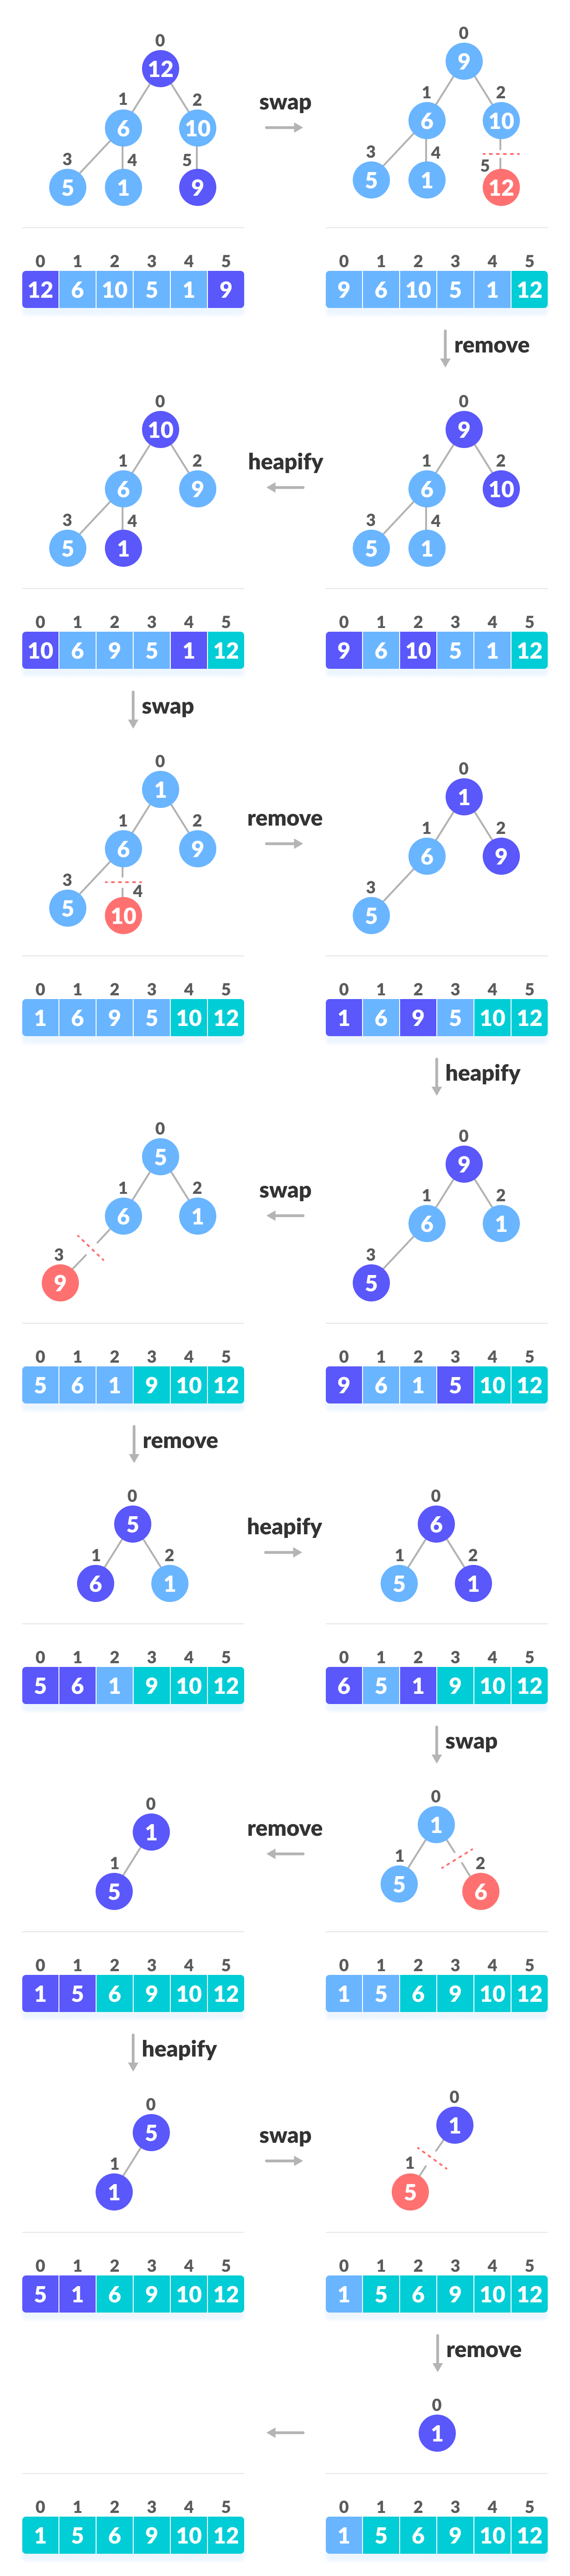
\includegraphics[scale = 0.189]{Pictures/heap_sort.jpeg}
        \caption{Veranschaulichung des Heapsort-Algorithmus}
        \label{fig:heapsort with array}
    \end{figure}

\subsection{Detaillierte Ansticht von AVL-Trees} \label{AVL-Trees-Anhang} 
\subsubsection{Entfernen:}
\subsubsection*{Fall 1}

Knoten $n$ hat zwei blätter als Kinder. Sei $p$ der Elternknoten von $n \implies $ Anderer Teilbaum hat Höhe $h' =$ 0, 1 oder 2.
\begin{itemize}
    \item $h' = $1: $bal(p)$ anpassen
    \item $h' = $0: $bal(p)$ anpassen. Aufruf von $upout(p)$
    \item $h' = $2: Rebalancieren des Teilbaumes. Aufruf von $upout(p)$
\end{itemize}



\subsubsection*{Fall 2}
Knoten $n$ hat einen inneren Knoten $k$ als Kind
\begin{itemize}
    \item Ersetze $n$ durch $k$ -  $upout(k)$ \ref{fig: upout(p)}
\end{itemize}



\subsubsection*{Fall 3}
Knoten $n$ hat zwei inneren Knoten als Kinder
\begin{itemize}
    \item Ersetze $n$ durch symmetrischen Nachfolger-  $upout(k)$ \ref{fig: upout(p)}
    \item Löschen des symmetrischen Nachfolgers wie in Fall 1 oder 2.
\end{itemize}


\subsubsection*{upout(p)}
Sei $pp$ der Elternknoten von $p$
\begin{itemize}
    \item $p$ linkes Kind von $pp$
        \begin{enumerate}
            \item $bal(pp) = -1 \implies bal(s) \gets 0 \ \textbf{$upout(pp)$}$
            \item $bal(pp) = 0 \implies bal(s) \gets 1 $
            \item $bal(pp) = +1 \implies $ (Vgl. unten \ref{fig: upout(p)})
        \end{enumerate}
    \item $p$ rechtes Kind von $pp$: Symmetrische Fälle unter Veratuschung von -1 und +1
\end{itemize}

\begin{figure}[h]
\centering
\begin{subfigure}{0.38\textwidth}
    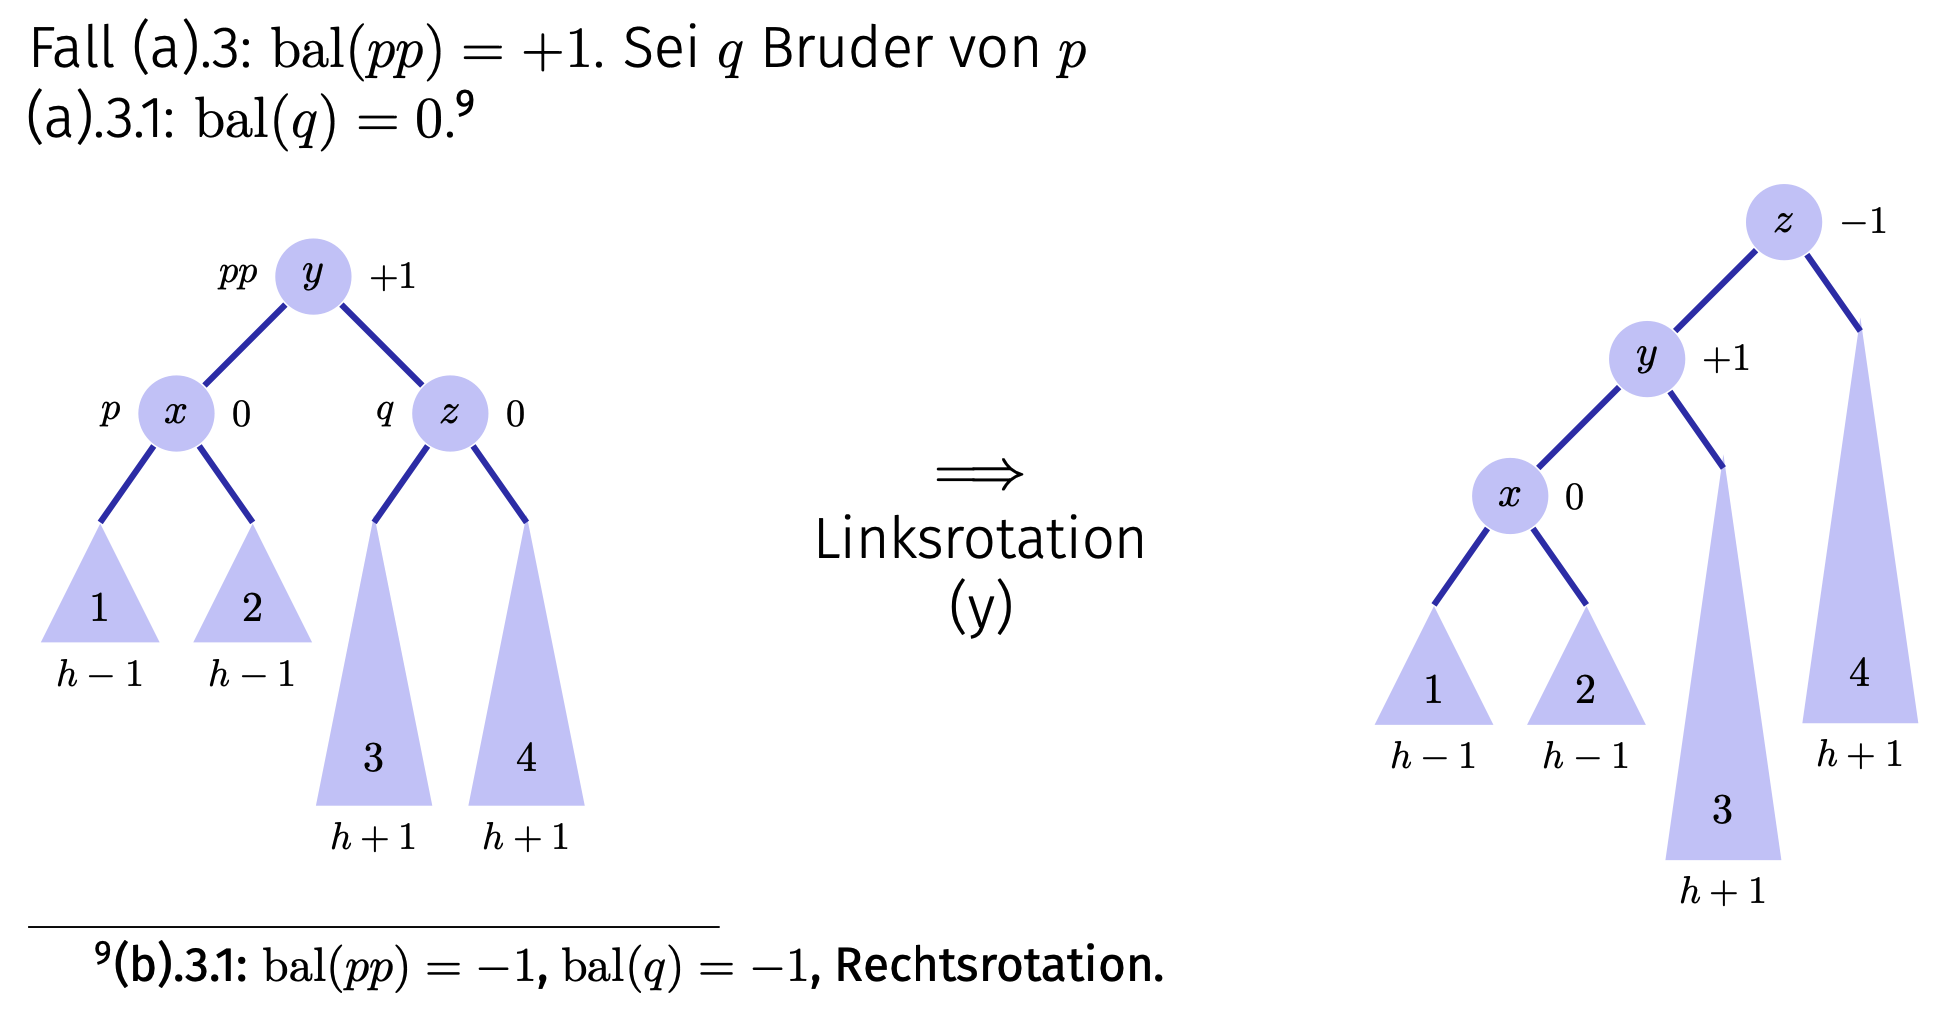
\includegraphics[width=\textwidth]{Pictures/upout1.png}
        \caption{Erster Schritt}
        \label{fig: upout1}
\end{subfigure}
\hfill
\begin{subfigure}{0.38\textwidth}
 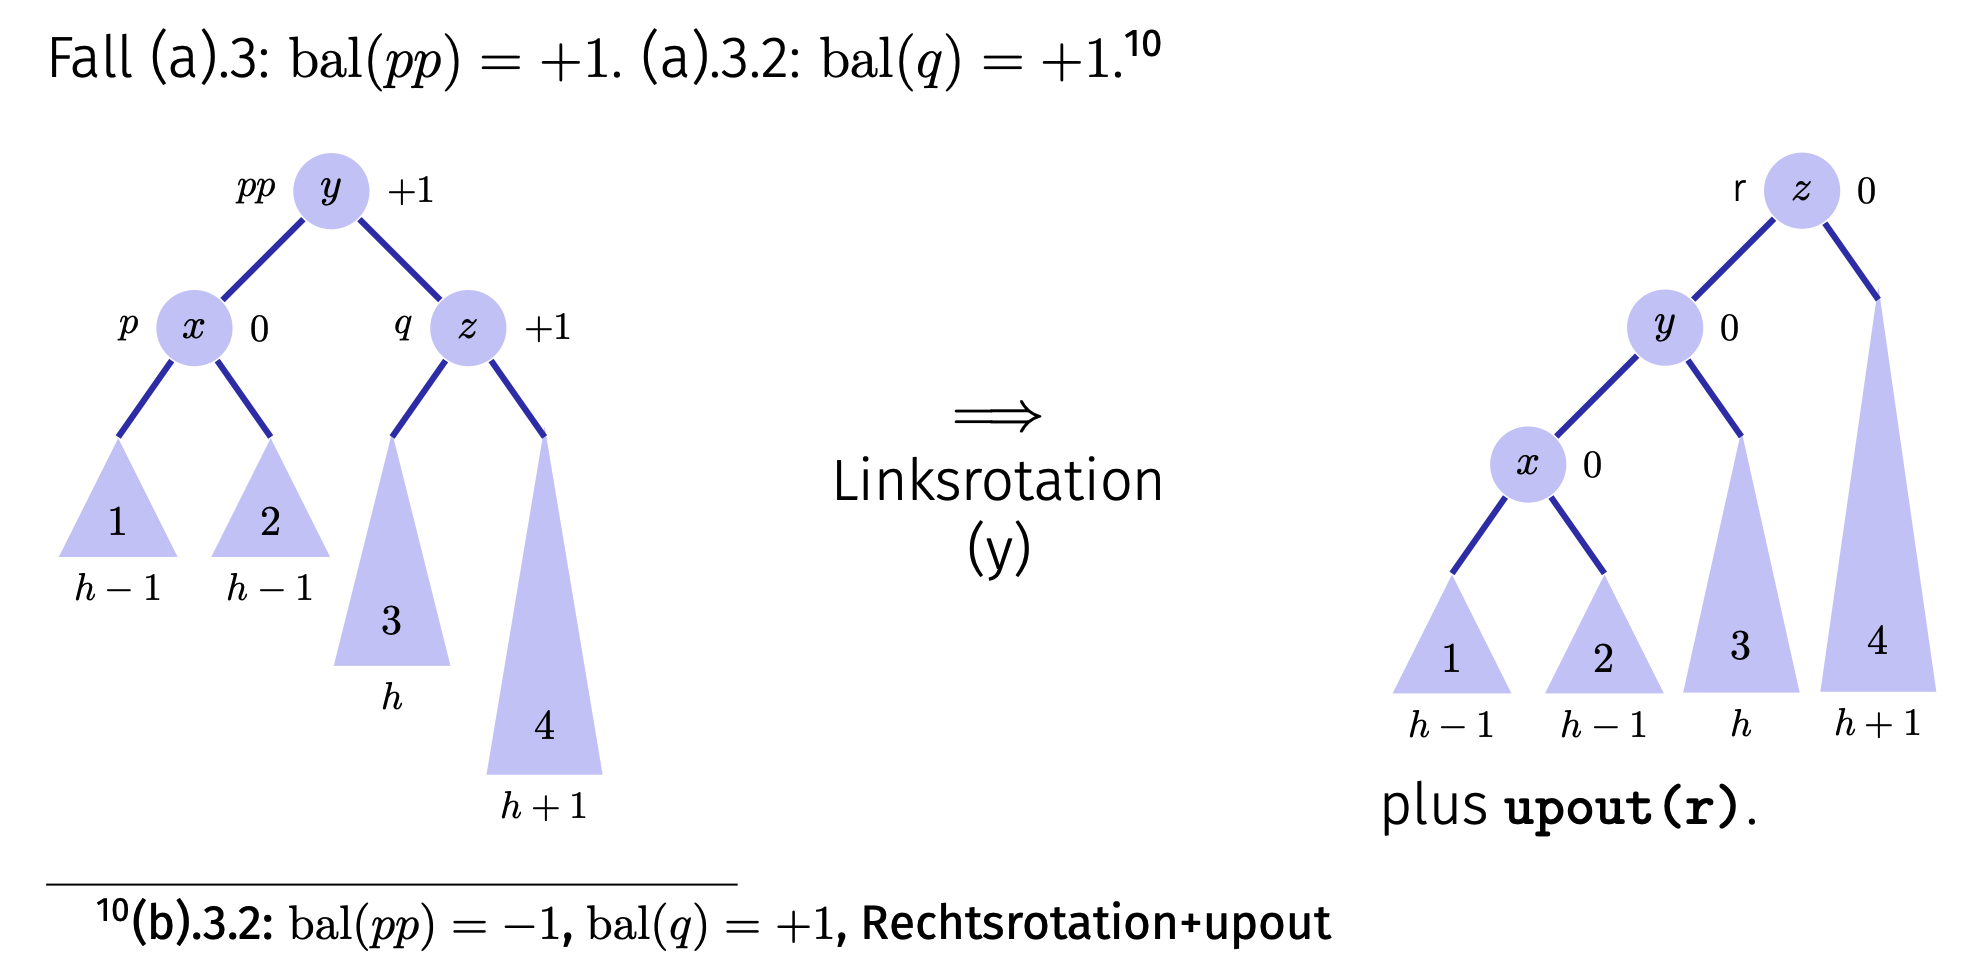
\includegraphics[width=\textwidth]{Pictures/upout2.png}  
 \caption{Zweiter Schritt}
        \label{fig: upout2}
\end{subfigure}

\begin{subfigure}{0.38\textwidth}
 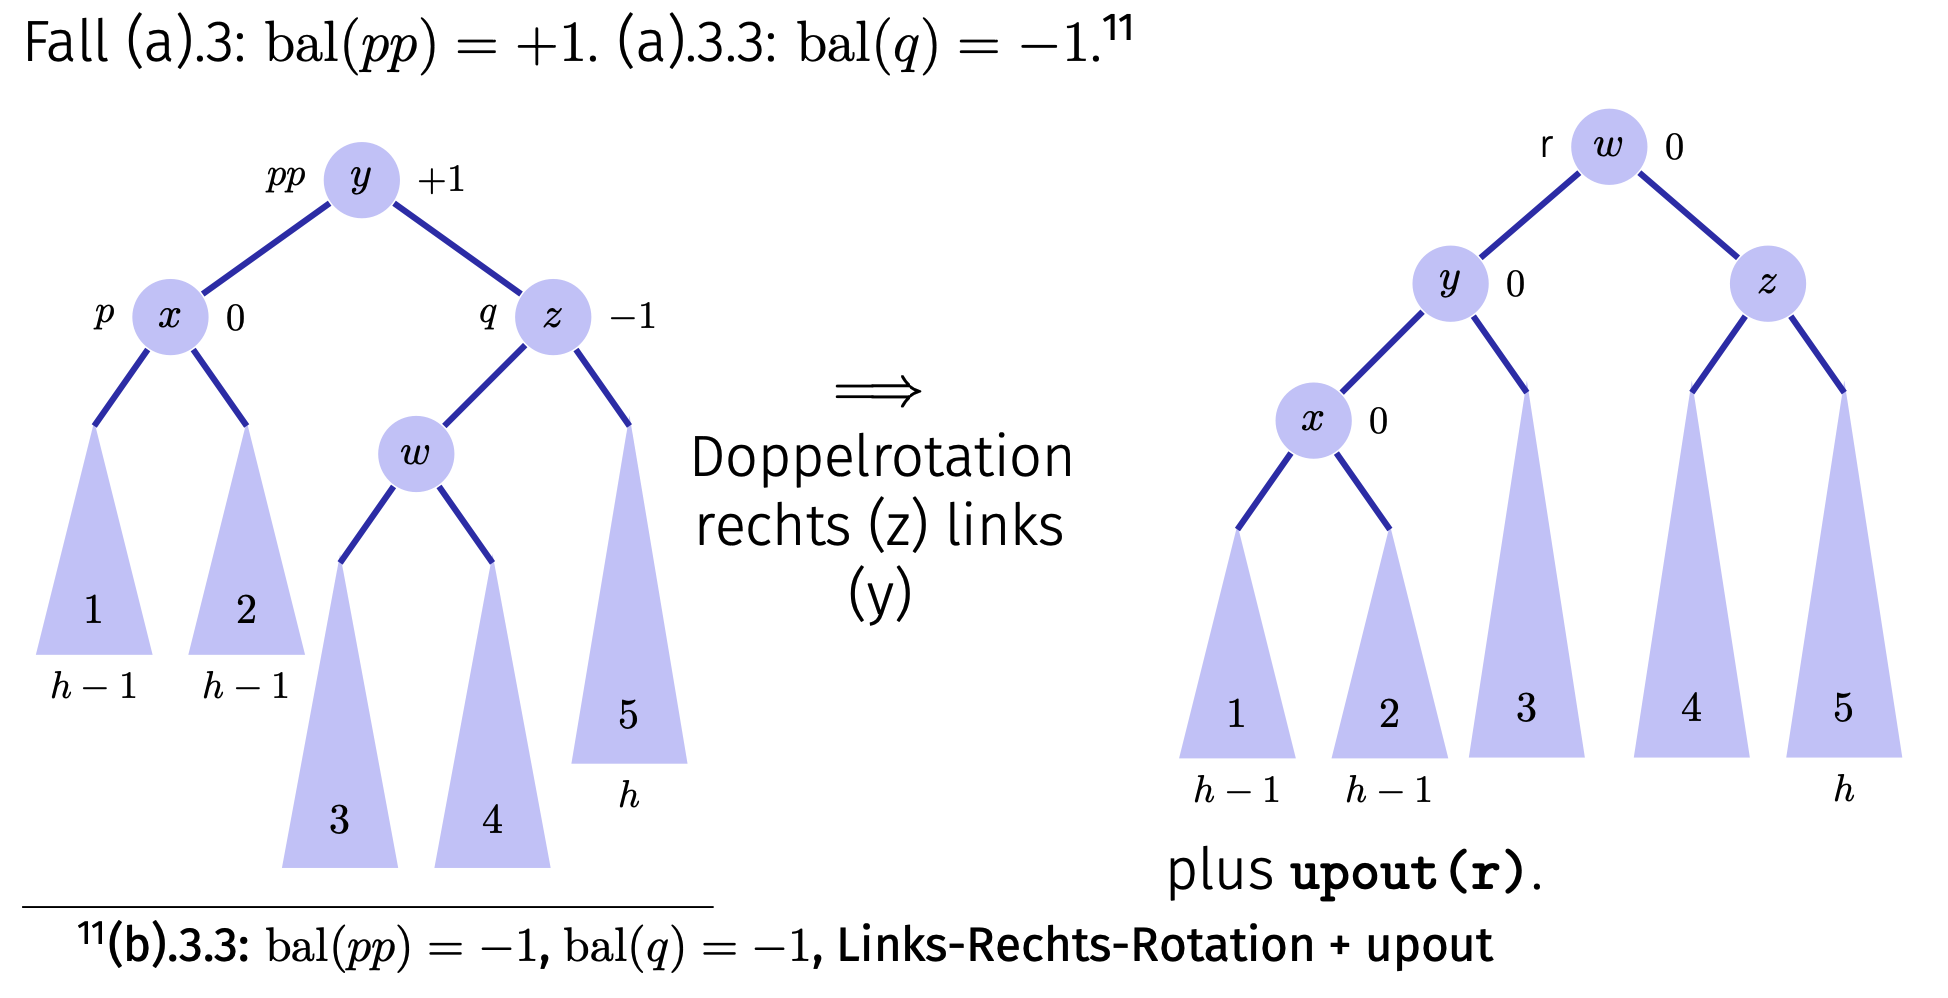
\includegraphics[width=\textwidth]{Pictures/upout3.png}
        \caption{Dritter Schritt}
        \label{fig: upout3}
\end{subfigure}
        
\caption{$upout(p)$, Mit (a) ist der Erste bullet point ($p$ linkes Kind von $pp$) gemeint}
\label{fig: upout(p)}
\end{figure}

\end{document}
